\chapter{EMJ Trigger Efficiency Study}
\label{chap:trigeff}

In previous searches for EMJs in CMS \cite{cmscollaborationSearchNewParticles2019, cmscollaborationSearchNewPhysics2024}, the trigger used for data collection was the $H_T$ trigger, with the latest one using a threshold of $1050\;\text{GeV}$\footnote{For data from 2016, a trigger that required at least one jet with $p_\text{T} > 450\;\text{GeV}$ or $H_T > 900\;\text{GeV}$ was used due to an issue where jets were being dropped from the $H_T$ sum if they reached the energy saturation of the L1 trigger. Because the data simulated correspond to the data collection conditions in 2022, this alternative trigger was not considered}, where $H_T$ is defined as the scalar sum of the transverse momentum of the jets in an the event. As a starting point, the efficiency of this previously used trigger was obtained for the EMJ simulated parameter space. The efficiency of trigger A is defined as

\begin{equation}
    \varepsilon(A) = \frac{N_{\text{A}}}{N_\text{T}},
\end{equation}

\noindent where $N_{\text{A}}$ are the number of events that pass the selection of trigger A, while $N_\text{T}$ corresponds to the total number of events. The uncertainty of these efficiencies was calculated using the Clopper-Pearson interval \cite{orawoConfidenceIntervalsBinomial2021}, which is an exact method. Figure \ref{fig:ht1050} shows the raw trigger efficiency maps for the HLT triggers, used by previous studies, for models with $X_{\text{dark}}$ and $Z'$ mediators for $m_{\pi_{\text{d}}} = 20 \;\text{GeV}$\footnote{While samples for $m_{\text{Med}}=10 \text{ GeV}$ were also used in this study, the conclusions drawn from those results are identical to the ones exposed in this chapter which were obtained from samples with $m_{\text{Med}}=20 \text{ GeV}$, so they are not shown here. The only noticeable difference was an overall decrease in all efficiency and efficiency improvements, as lower mass correlates with less energetic EMJ.}.

\begin{figure}[h]
    \centering
    \begin{subfigure}{0.45\textwidth}
        \includesvg[width=\linewidth]{images/HLT/trigeffplots2D_HLT_efftype-trig_mDark-20_t-channel_HLT_PFHT1050_effs}
    \end{subfigure}
    \hfill
    \begin{subfigure}{0.45\textwidth}
        \includesvg[width=\linewidth]{images/HLT/trigeffplots2D_HLT_efftype-trig_mDark-20_s-channel_HLT_PFHT1050_effs}
    \end{subfigure}
    \caption{Trigger efficiency of \texttt{HLT\_PFHT1050} for the simulated parameter space.}
    \label{fig:ht1050}
\end{figure}

It is readily apparent that the performance of this trigger for shorter and longer dark pion lifetimes is comparable in the case of the $X_{\text{dark}}$ mediator. This is to be expected, as the final state has a high jet multiplicity and, even for models with higher $c\tau$, two of the four jets are QCD jets, so the event can easily be triggered on by $H_T$ triggers. On the other hand, for the $Z'$ model, while the efficiency is high towards a lower dark pion proper decay length and higher mediator mass, for the rest of the parameter space, the efficiency drops considerably. This is likely in part due to the fact that a higher portion of the jet energy is deposited outside the calorimeters for higher lifetimes. Similar observations made with the \texttt{HLT\_PFHT1050} trigger can be made for its L1 seed, the \texttt{L1\_HTT450er}, the efficiency heatmaps for which can be seen in Figure \ref{fig:htt450er}.

\begin{figure}[h]
    \centering
    \begin{subfigure}{0.45\textwidth}
        \includesvg[width=\linewidth]{images/L1/trigeffplots2D_L1_efftype-trig_mDark-20_t-channel_L1_HTT450er_effs.svg}
    \end{subfigure}
    \hfill
    \begin{subfigure}{0.45\textwidth}
        \includesvg[width=\linewidth]{images/L1/trigeffplots2D_L1_efftype-trig_mDark-20_s-channel_L1_HTT450er_effs.svg}
    \end{subfigure}
    \caption{Trigger efficiency of \texttt{L1\_HTT450er} for the simulated parameter space}
    \label{fig:htt450er}
\end{figure}

These results show the potential for an improvement in the sensitivity of EMJs in a Run 3 search, particularly for the $Z'$ model. To understand what the set of LLP and AD triggers under study has to offer in terms of increasing sensitivity, the efficiency of the conventional triggers with the highest efficiency for each point in the simulated parameter space was used as a baseline. Conventional triggers in this context refer to the set of all triggers in the selected 2022 trigger menu that are not in the group of triggers under study or in a list of special-purpose triggers that are not relevant to these studies. Moreover, all triggers studied are unprescaled for the data-taking period the data is simulated for, and only those paths corresponding to nominal operations are included. For each trigger, the efficiency increases, or $\text{EI}$, defined as

\begin{equation}
    \text{EI}_{\text{A}B} (m_{\text{Med}}, m_{\pi_{\text{d}}},c\tau_{\pi_{\text{d}}}) = \frac{\varepsilon_{\text{A OR B}}}{\varepsilon_{\text{B}}},
\end{equation}

\noindent is used as a measure of increased sensitivity, where $\text{A}$ is the trigger under study, and $\text{B}$ is the best conventional trigger for the given set of parameter values.

The choice of L1 (Table \ref{tab:l1-trigs}) triggers for this study is based on their novelty compared to what was available for the previous search for EMJ, and with their functionality in mind. The anomaly detection triggers allow for a model-independent way of selecting anomalous events with exotic signatures. Moreover, previous studies \cite{govorkovaAutoencodersFPGAsRealtime2022} have shown that the use of this set of triggers for the search of beyond Standard Model physics can provide some increase in sensitivity. However, because the models which give rise to EMJs predict long-lived particles in the dark sector, potential was seen for triggers targeting signatures left behind by long-lived particles. Previous studies, as well as their targeted nature, have reinforced this hypothesis \cite{CMS-DP-2024-058} and therefore motivate their inclusion in this study.

\section{Anomaly Detection Triggers}
% \noindent\textbf{Anomaly Detection Triggers:} 

As described in detail in \cite{govorkovaAutoencodersFPGAsRealtime2022}, these triggers utilize unsupervised ML techniques to apply a model-independent selection of events with potentially interesting physics that would otherwise not be selected by cut-based triggers or triggers targeting particular detector signatures. However, due to resource constraints in the L1 system and the challenges of fitting a complex ML model in an FPGA, various techniques such as quantized aware training and knowledge distillation must be implemented to deploy these triggers.

The two AD triggers considered in these studies are AXOL1TL, based on a variational autoencoder, and CICADA, based on a convolutional autoencoder. They were trained on a large unbiased sample of data, most of which amounts to known QCD physics or where there was little momentum transfer, and output an anomaly score which serves as a metric of how different an output event is from the typical events the model was trained on. However, the input to AXOL1TL and CICADA differ: the former uses L1 objects, namely the $p_T$, $\phi$ and $\eta$ of 4 $e/\gamma$, 4 $\mu$ and 10 jets, as well as the $\phi$ and magnitude of the event's missing transverse energy, while the latter uses as input the calorimeter region energies. A threshold is applied to the anomaly score output, which dictates whether or not an event is selected, and which allows for the control of the rate of the trigger itself, as a higher threshold implies a less likelihood for any particular event to meet the selection criteria.

In order to first understand which areas of parameter space AXOL1TL targets for each model, we first looked at the trigger efficiency heatmaps that can be seen in Figure \ref{fig:axol1tl_trig_tchan} and Figure \ref{fig:axol1tl_trig_schan}. These figures show that AXOL1TL is more sensitivities to lower dark pion lifetimes, as well as higher mediator masses. This result was not unexpected, as those regions of parameter space are, in general, the "easiest" to trigger on. When combining AXOL1TL with the best triggers, we see that the results seem relatively unchanged with respect to Figure \ref{fig:htt450er}, as can bee sen in Figure \ref{fig:axol1tl_trigplusbest_tchan} and \ref{fig:axol1tl_trigplusbest_schan}, as those same regions to which AXOL1TL targets overlap with those to which the set of best conventional triggers is sensitive. 

While the previous observations might initially paint the picture that AXOl1TL offers little in terms of increasing our sensitivity for EMJs in the harder to trigger on regions (i.e., lower mediator mass, higher dark pion lifetimes), a look at improvement plots in Figure \ref{fig:axol1tl_improv_tchan} and Figures \ref{fig:axol1tl_improv_schan} show that AXOL1TL does provide some increase efficiency for these regions, particularly for the lower mediator masses. Figure \ref{fig:axol1tl_eff1D_tchan} and \ref{fig:axol1tl_eff1D_schan} show the efficiency as a function of $c\tau_{\text{dark}}$ for the mediator masses in which the $\text{EI}$ peaks for the bifundamental and Z' mediator models. In these plots, we can see that for the bifundamental model $\text{EI}$ has a peak value of approximately $1.23\times$ and $1.45\times$ for the Z' mediator model. 

\begin{figure}[h]
  \centering

  % Bifundamental mediator model (t-channel)
  \begin{subfigure}[t]{0.45\textwidth}
    \centering
    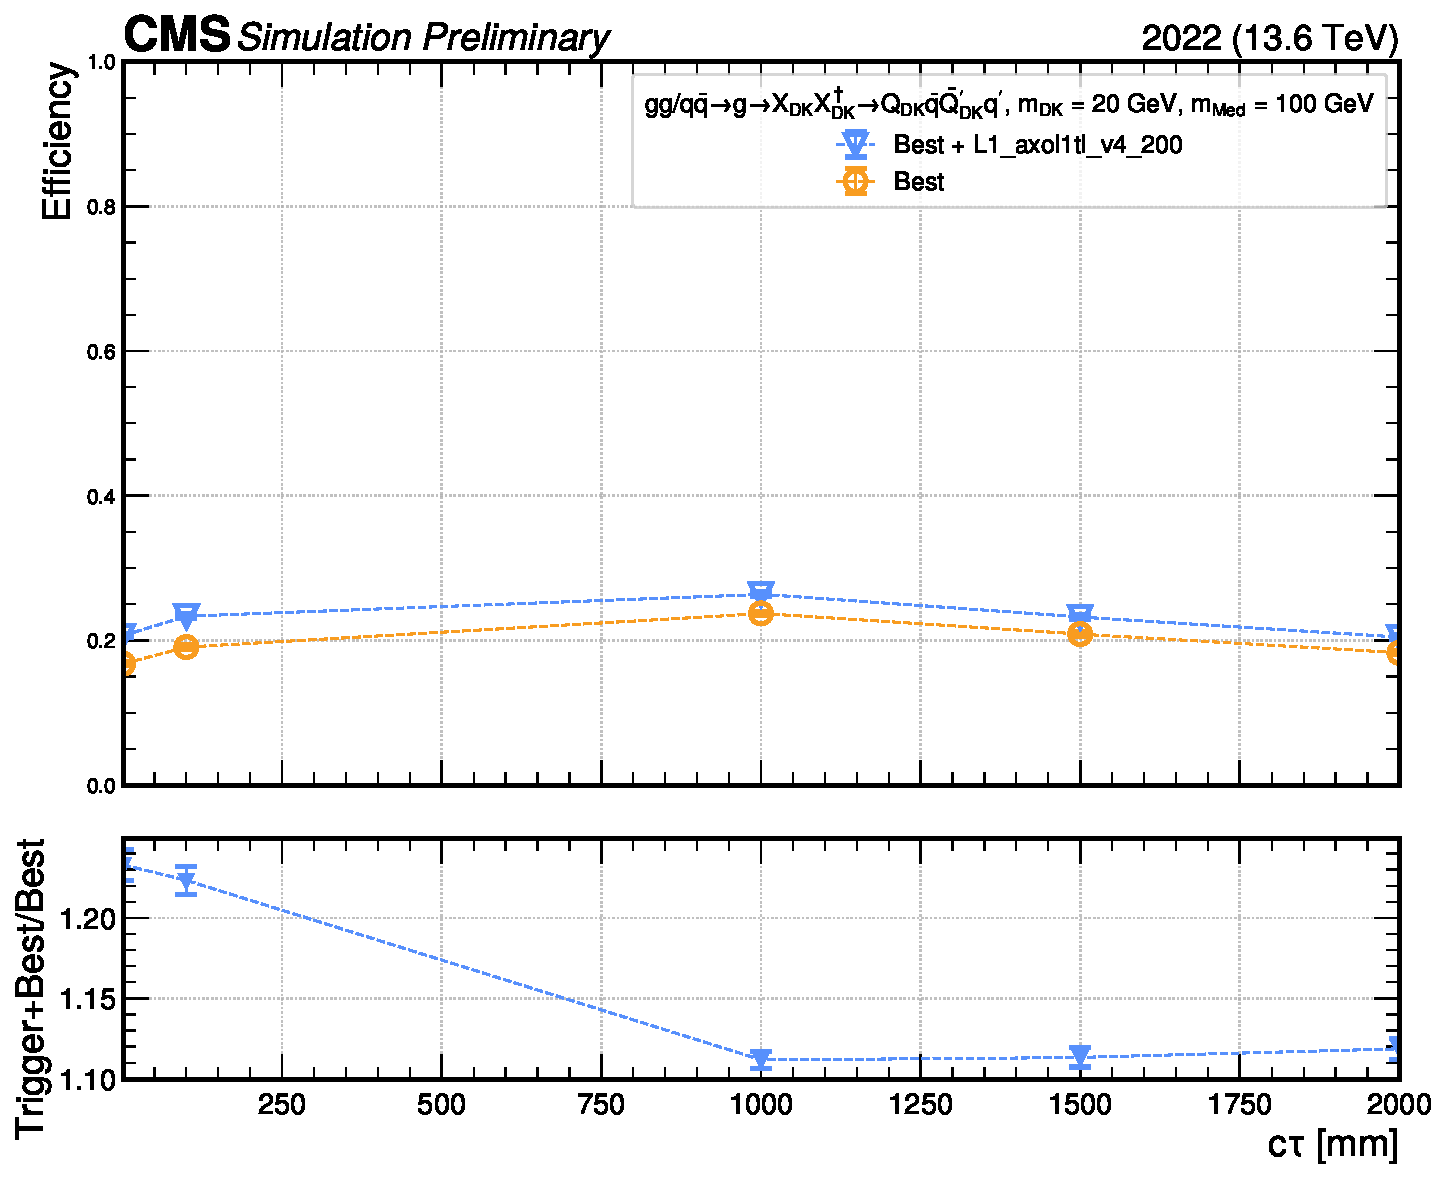
\includegraphics[width=\linewidth]{images/L1/ad_1D_tchan/trigeffplots1D_L1_efftype-trigplusbest_t-channel_mDark-20_mMed-100_L1_axol1tl_v4_200_study_cloppear.pdf}
    \caption{Bifundamental mediator model: Trigger+best object efficiency vs.\ $c\tau$ at $m_\mathrm{med} = 100$ GeV (peak improvement)}
    \label{fig:axol1tl_eff1D_tchan}
  \end{subfigure}
  \hfill
  % Z' mediator model (s-channel)
  \begin{subfigure}[t]{0.45\textwidth}
    \centering
    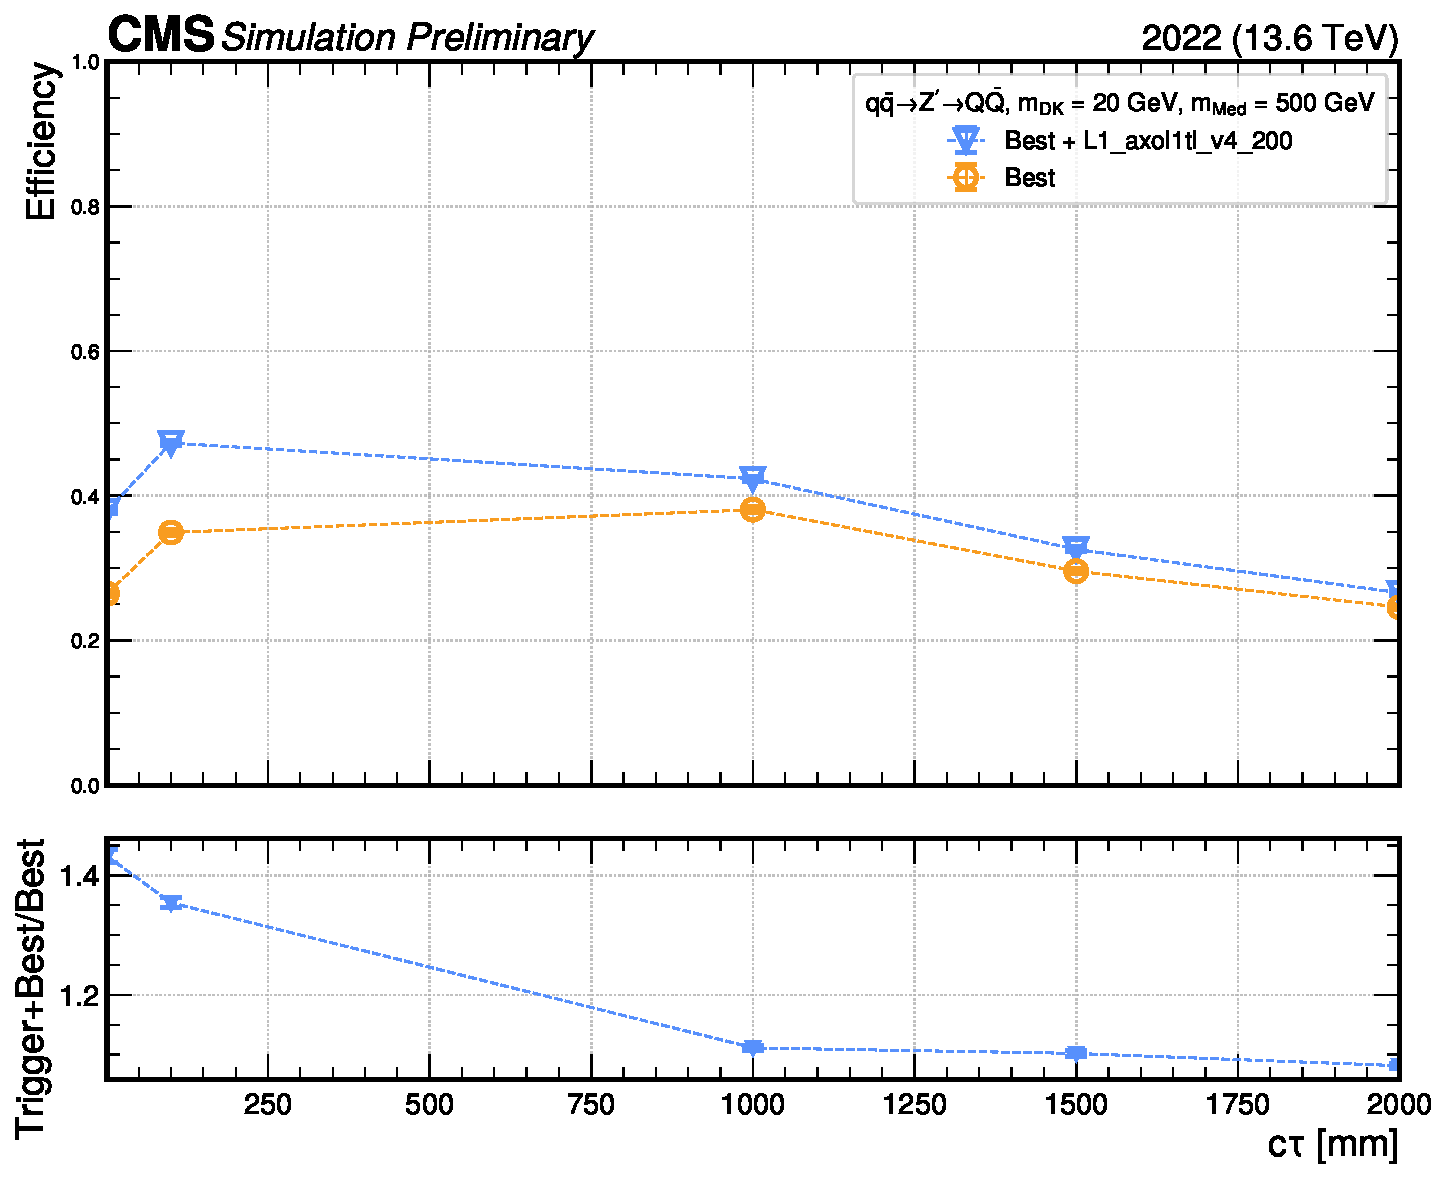
\includegraphics[width=\linewidth]{images/L1/ad_1D_schan/trigeffplots1D_L1_efftype-trigplusbest_s-channel_mDark-20_mMed-500_L1_axol1tl_v4_200_study_cloppear.pdf}
    \caption{Z' mediator model: Trigger+best object efficiency vs.\ $c\tau$ at $m_\mathrm{med} = 500$ GeV (peak improvement)}
    \label{fig:axol1tl_eff1D_schan}
  \end{subfigure}

  \caption{Trigger+best object efficiency as a function of dark pion lifetime $c\tau$ using AXOL1TL, for $m_\mathrm{dark} = 20$ GeV. Each curve corresponds to the mediator mass that yielded the maximum improvement in efficiency for the respective model.}
  \label{fig:axol1tl_eff1D}
\end{figure}

\begin{figure}[h]
  \centering

  % Trigger-only
  \begin{subfigure}[t]{0.45\textwidth}
    \centering
    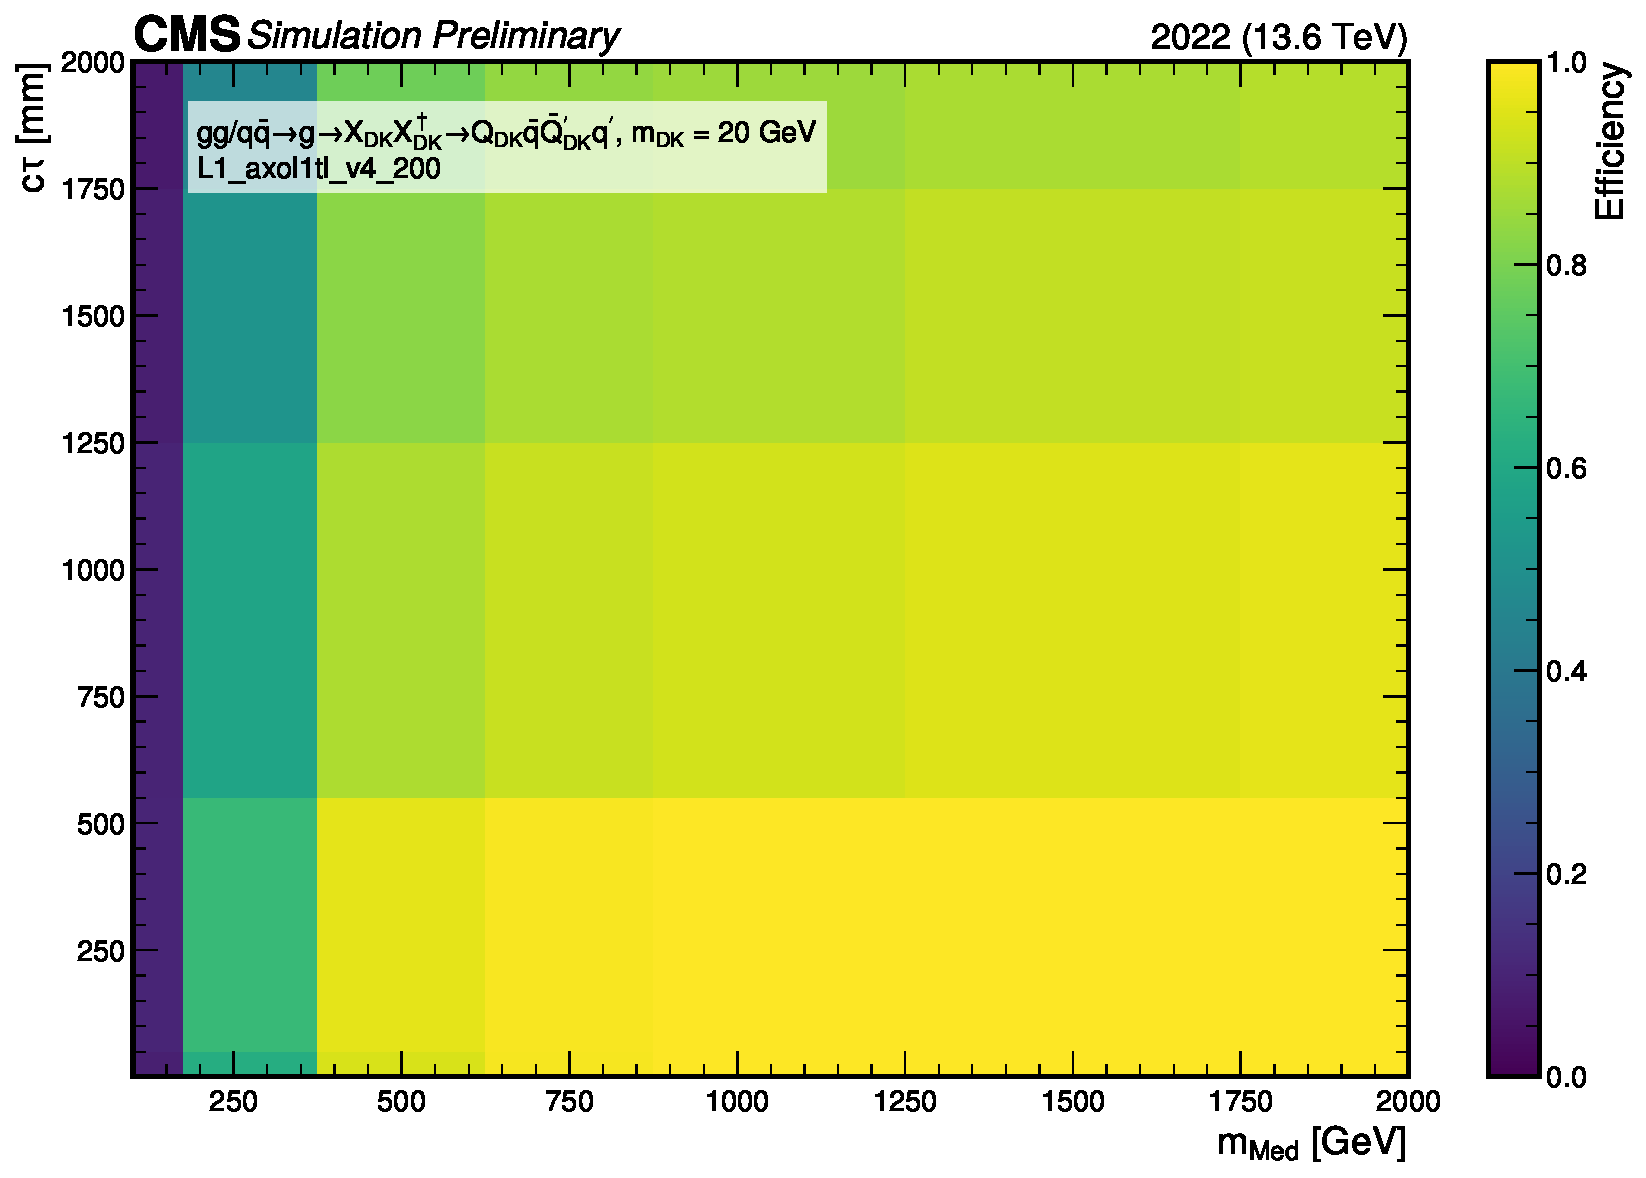
\includegraphics[width=\linewidth]{images/L1/ad_2D_tchan/trigeffplots2D_L1_efftype-trig_t-channel_mDark-20_L1_axol1tl_v4_200_study_cloppear.pdf}
    \caption{Trigger-only, Bifundamental mediator model}
    \label{fig:axol1tl_trig_tchan}
  \end{subfigure}
  \hfill
  \begin{subfigure}[t]{0.45\textwidth}
    \centering
    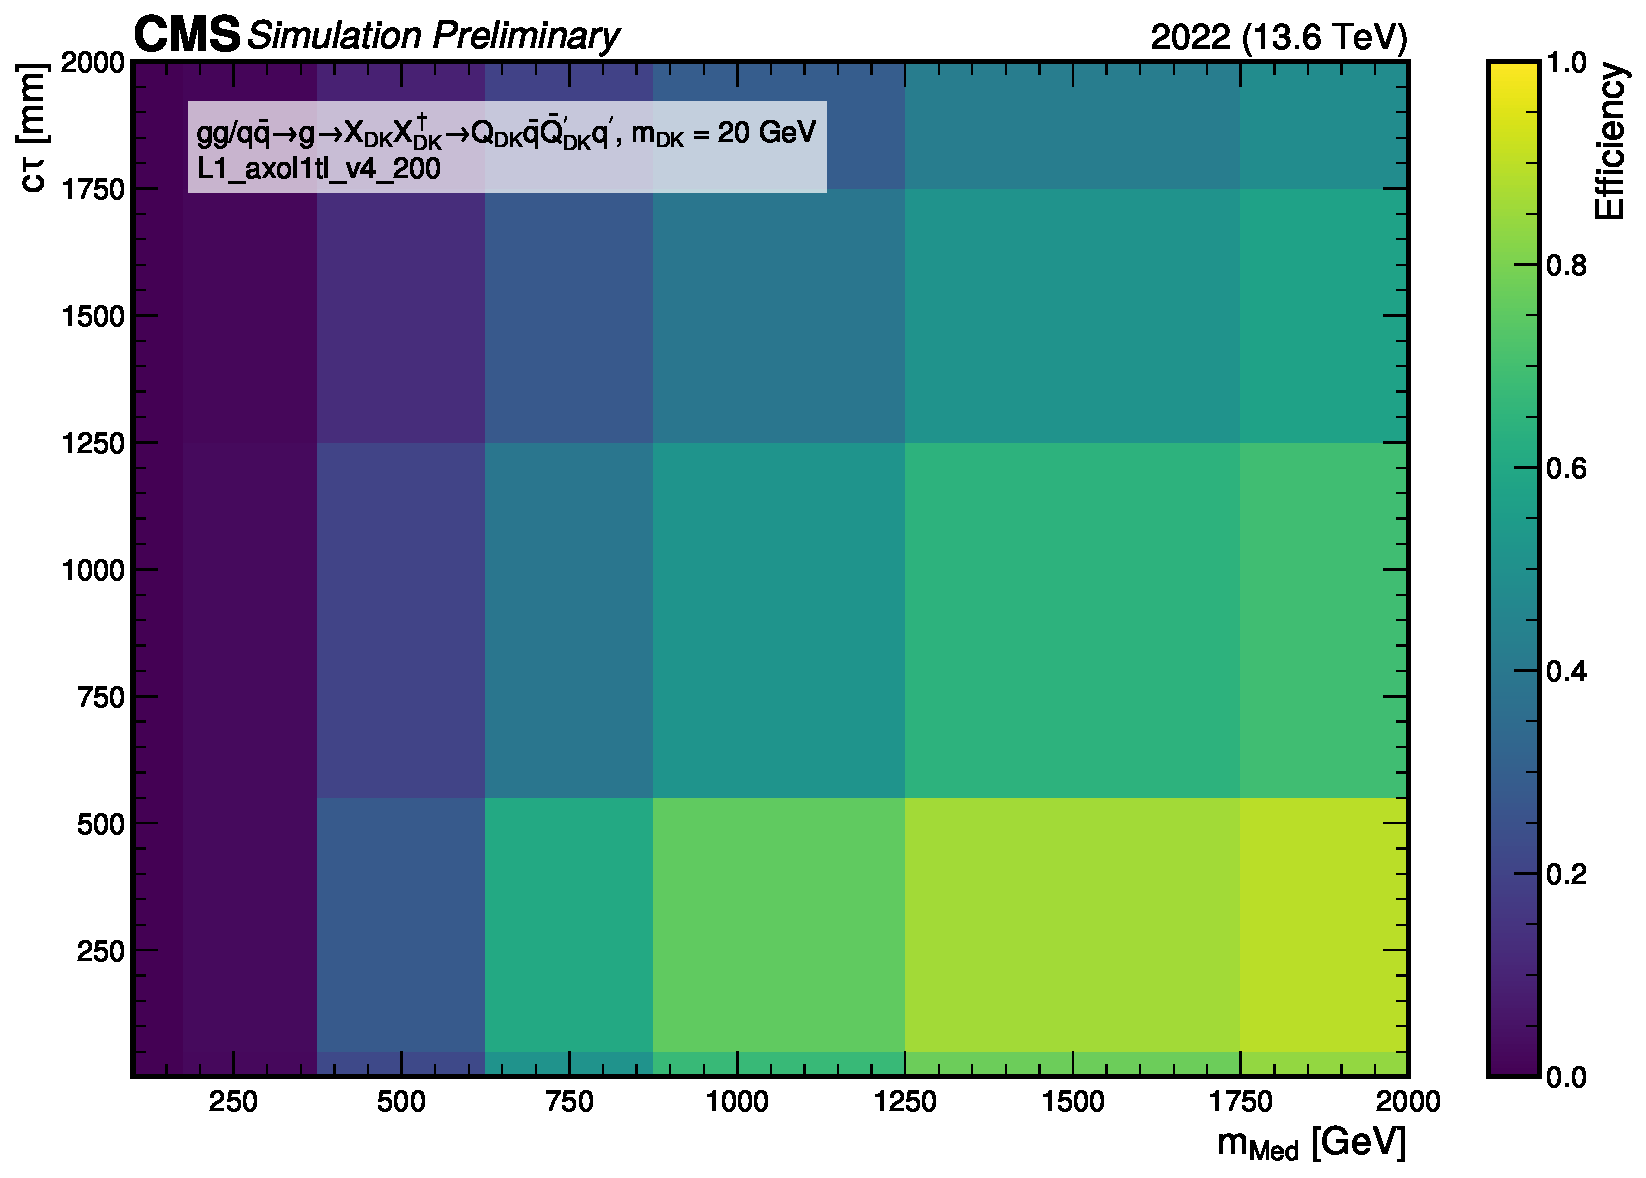
\includegraphics[width=\linewidth]{images/L1/ad_2D_schan/trigeffplots2D_L1_efftype-trig_s-channel_mDark-20_L1_axol1tl_v4_200_study_cloppear.pdf}
    \caption{Trigger-only, Z' mediator model}
    \label{fig:axol1tl_trig_schan}
  \end{subfigure}

  \vspace{1em}

  % Trigger+best
  \begin{subfigure}[t]{0.45\textwidth}
    \centering
    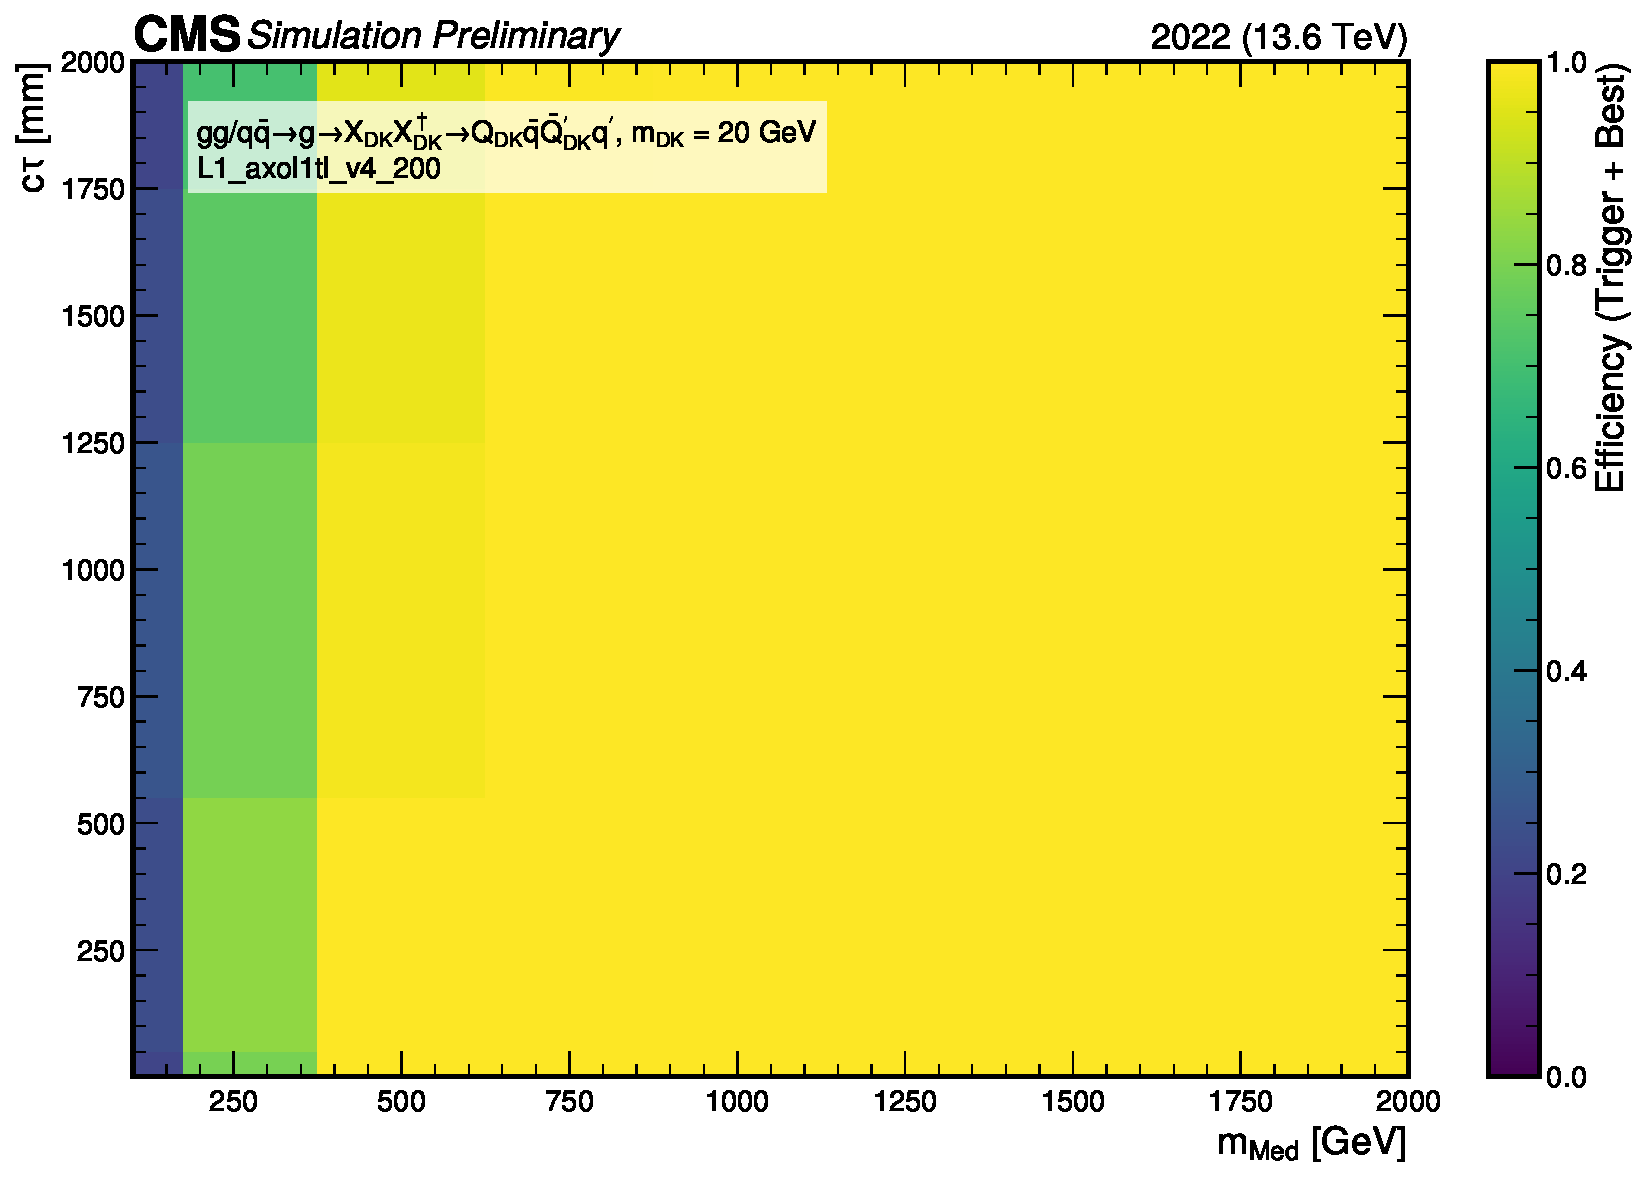
\includegraphics[width=\linewidth]{images/L1/ad_2D_tchan/trigeffplots2D_L1_efftype-trigplusbest_t-channel_mDark-20_L1_axol1tl_v4_200_study_cloppear.pdf}
    \caption{Trigger+best, Bifundamental mediator model}
    \label{fig:axol1tl_trigplusbest_tchan}
  \end{subfigure}
  \hfill
  \begin{subfigure}[t]{0.45\textwidth}
    \centering
    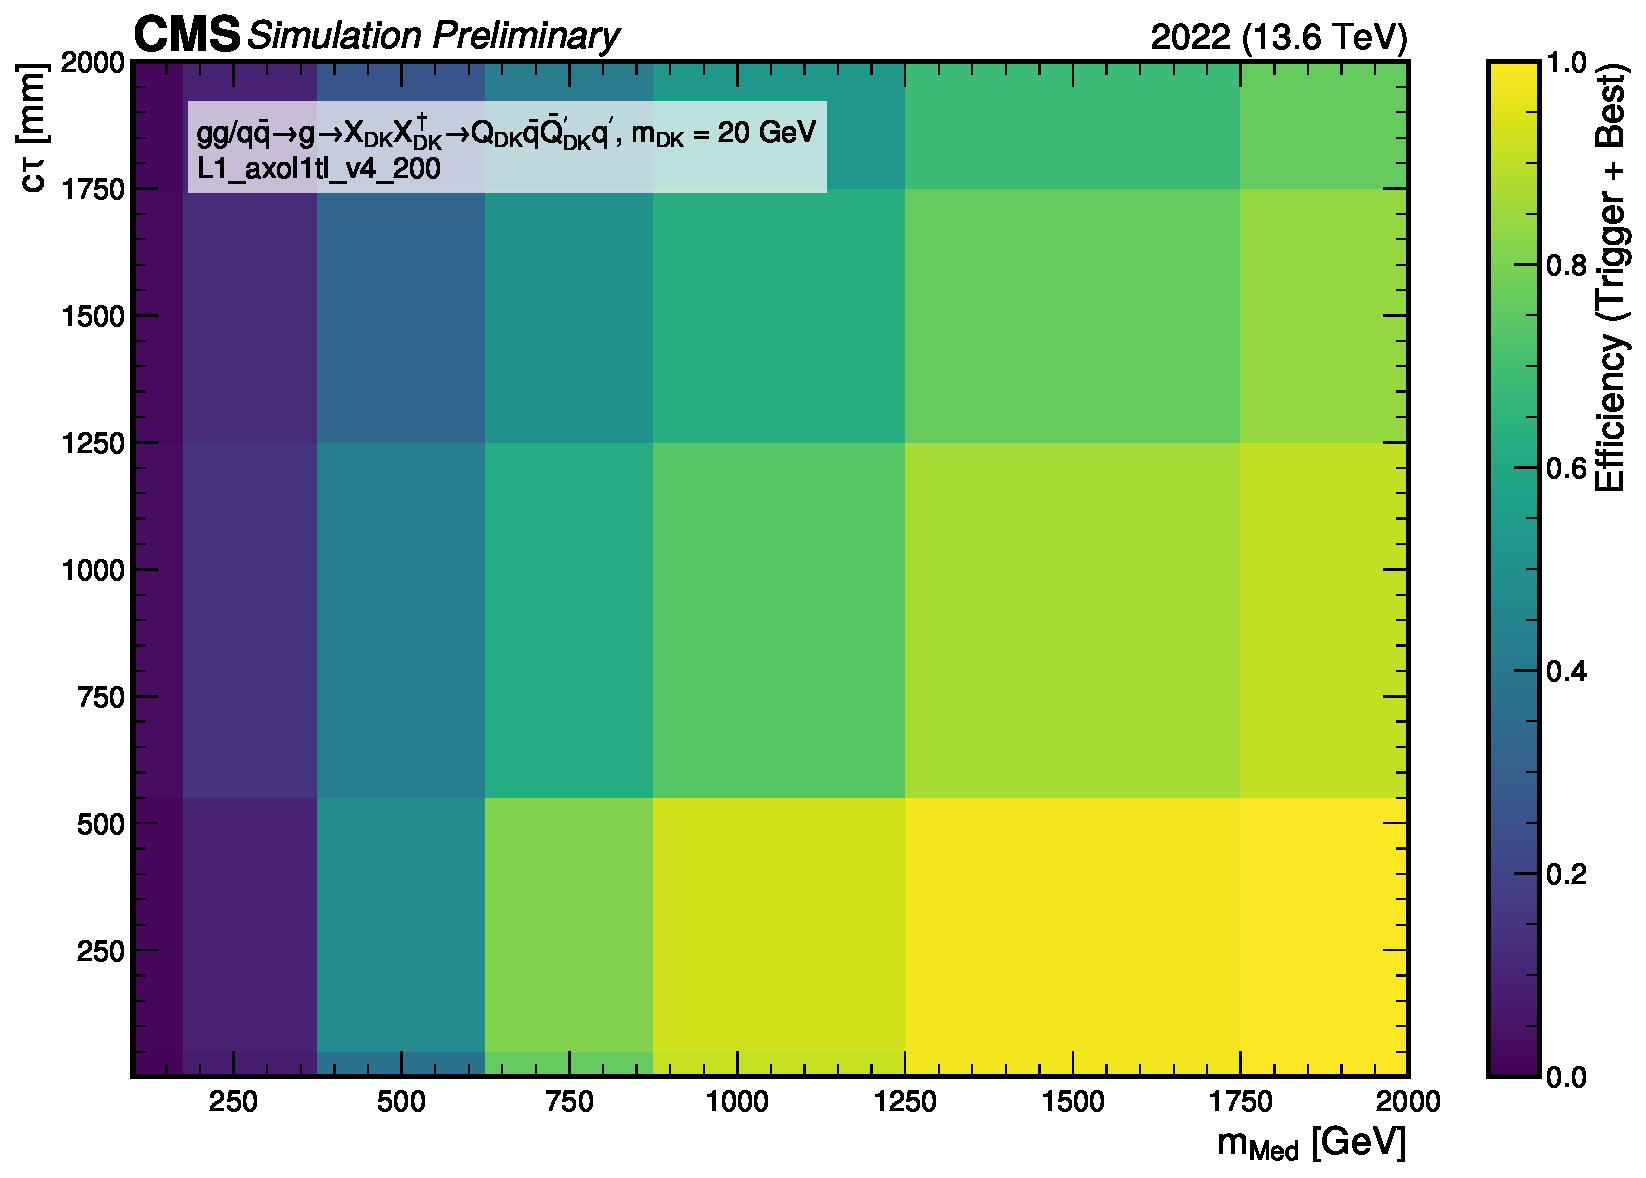
\includegraphics[width=\linewidth]{images/L1/ad_2D_schan/trigeffplots2D_L1_efftype-trigplusbest_s-channel_mDark-20_L1_axol1tl_v4_200_study_cloppear.pdf}
    \caption{Trigger+best, Z' mediator model}
    \label{fig:axol1tl_trigplusbest_schan}
  \end{subfigure}

  \vspace{1em}

  % Improvement
  \begin{subfigure}[t]{0.45\textwidth}
    \centering
    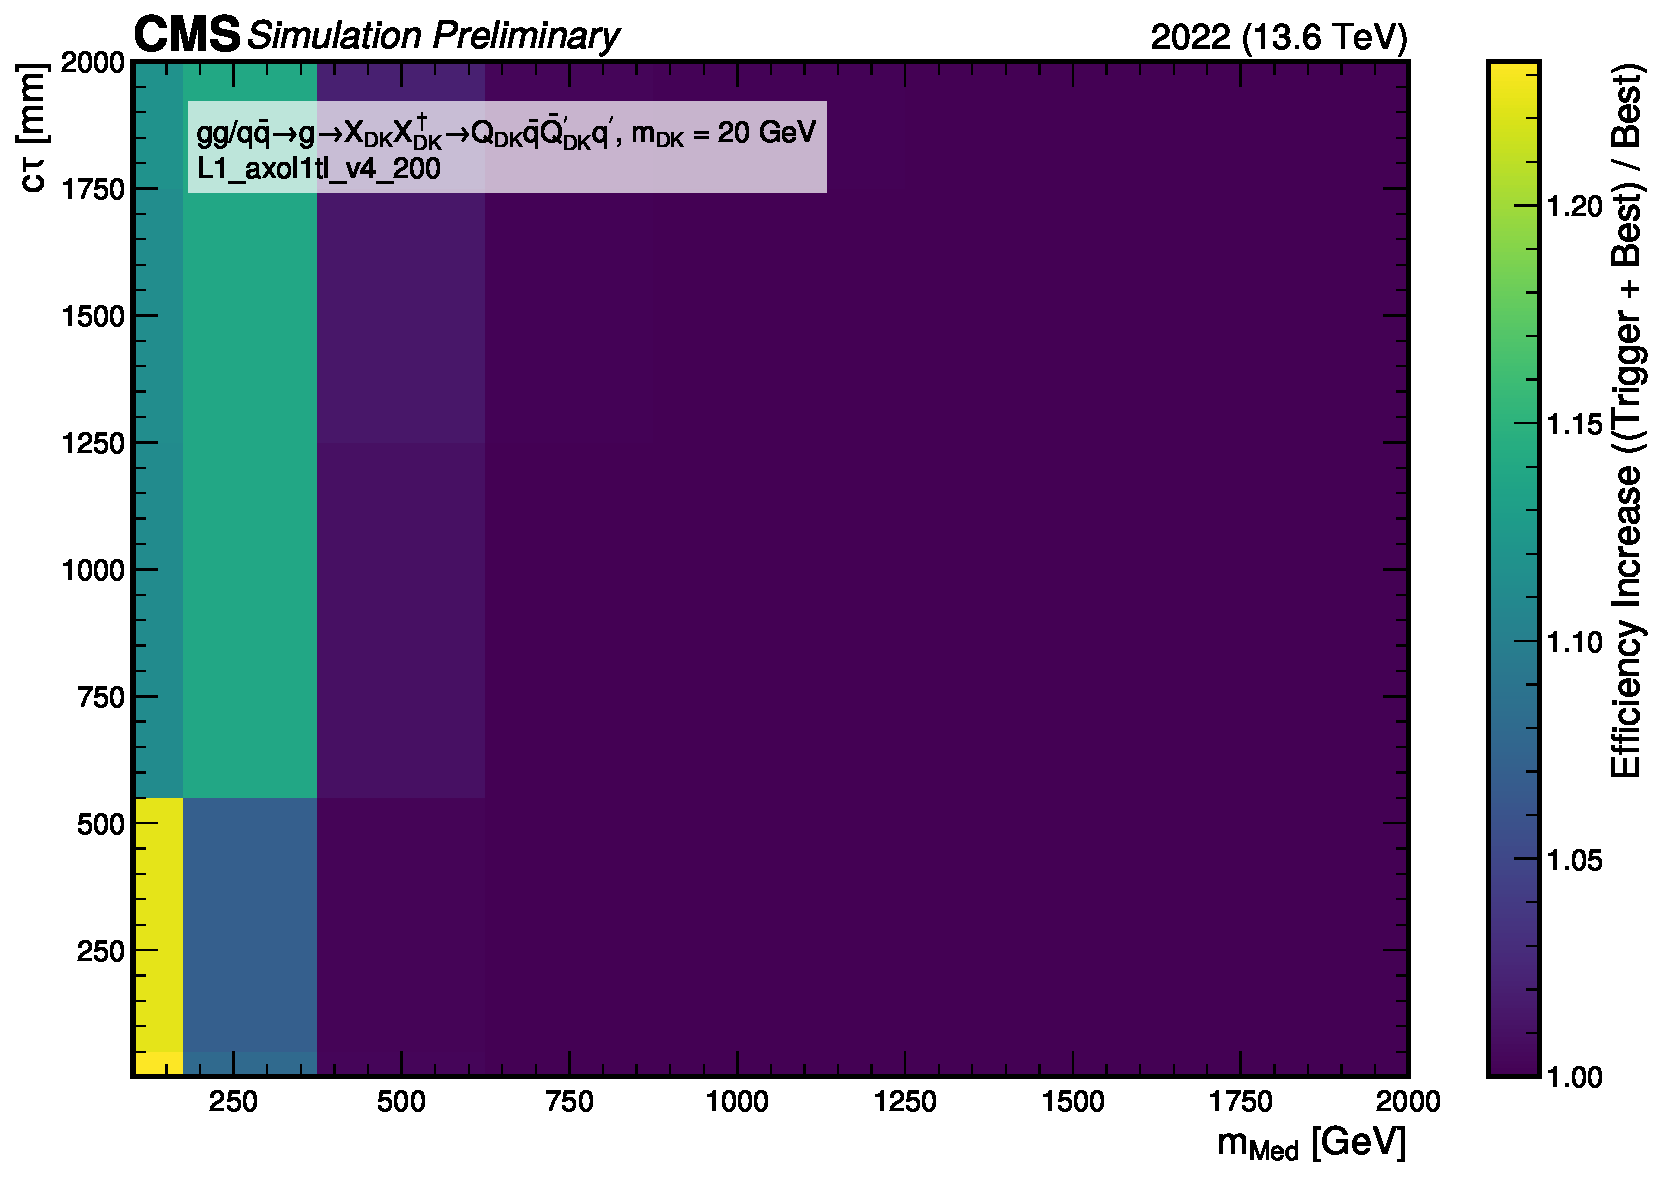
\includegraphics[width=\linewidth]{images/L1/ad_2D_tchan/trigeffplots2D_L1_efftype-improv_t-channel_mDark-20_L1_axol1tl_v4_200_study_cloppear.pdf}
    \caption{Improvement, Bifundamental mediator model}
    \label{fig:axol1tl_improv_tchan}
  \end{subfigure}
  \hfill
  \begin{subfigure}[t]{0.45\textwidth}
    \centering
    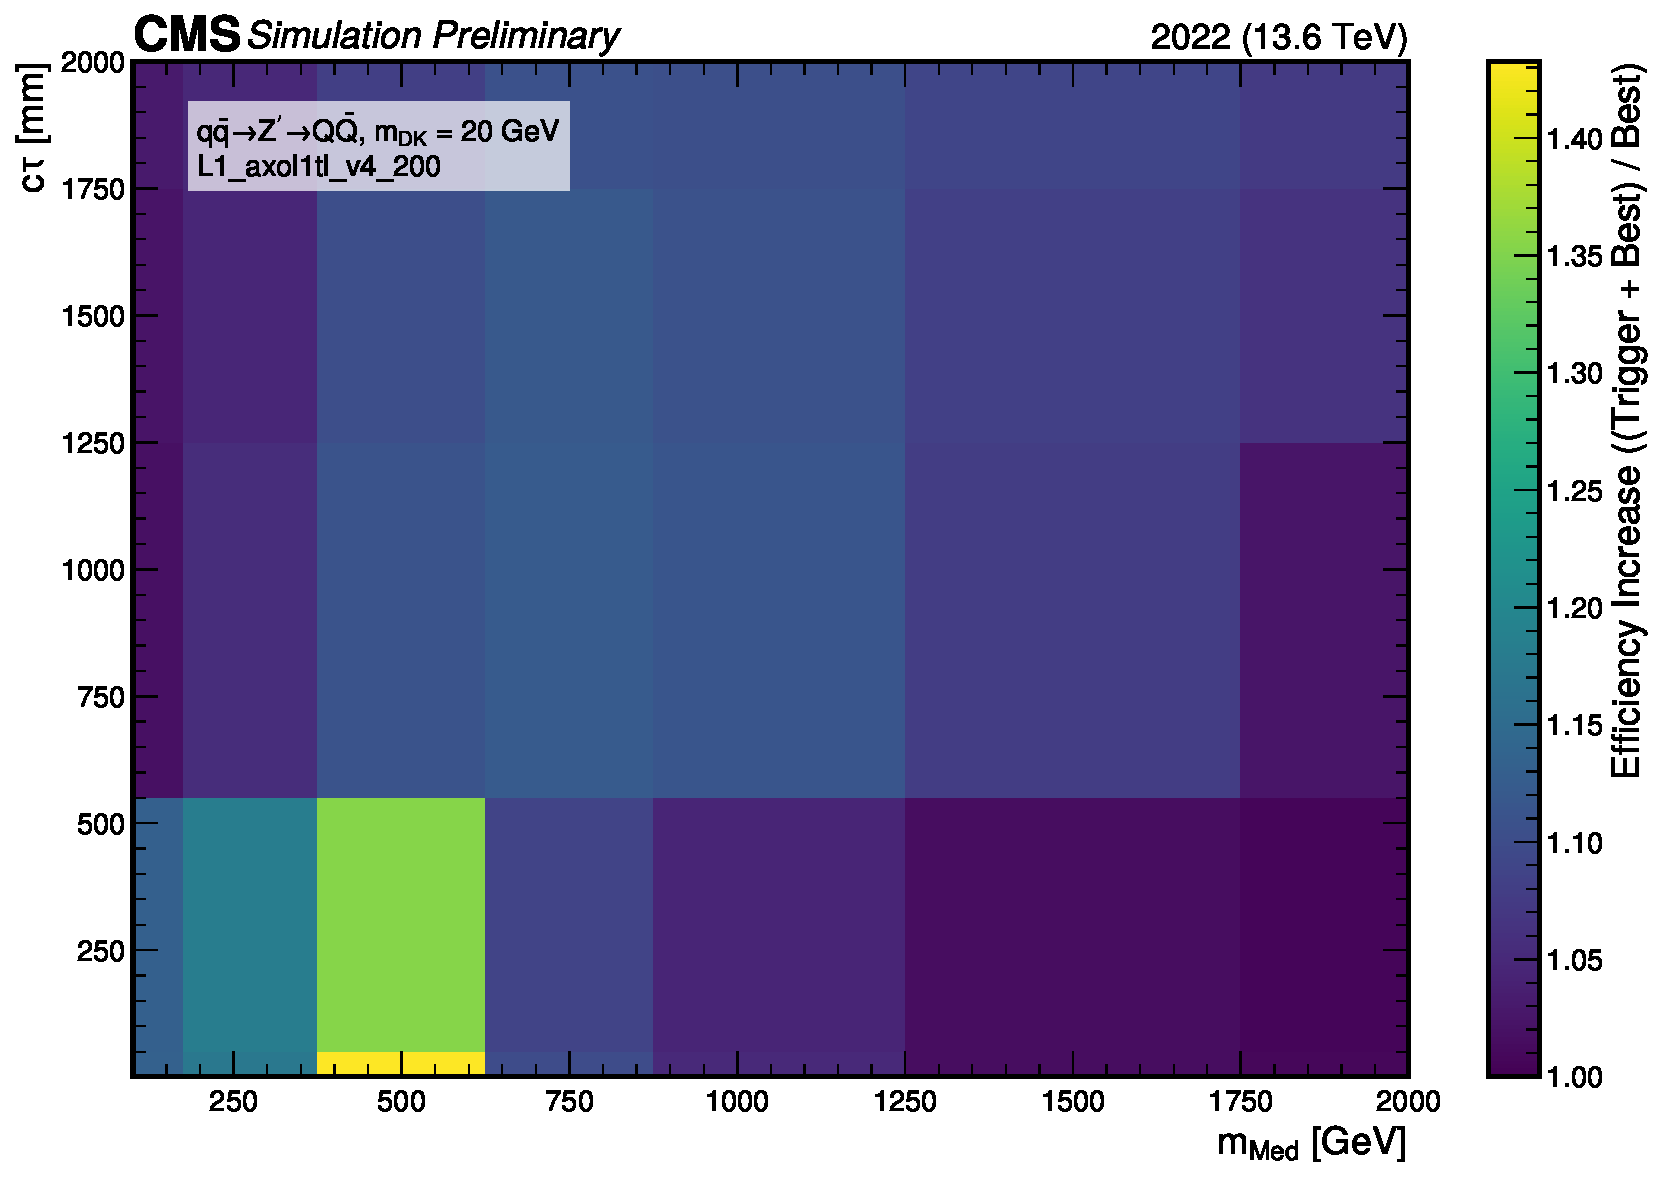
\includegraphics[width=\linewidth]{images/L1/ad_2D_schan/trigeffplots2D_L1_efftype-improv_s-channel_mDark-20_L1_axol1tl_v4_200_study_cloppear.pdf}
    \caption{Improvement, Z' mediator model}
    \label{fig:axol1tl_improv_schan}
  \end{subfigure}

  \caption{AXOL1TL trigger efficiency heatmaps for $m_\mathrm{dark} = 20$ GeV in both the bifundamental mediator model and the Z' mediator model.}
  \label{fig:axol1tl_eff}
\end{figure}

For CICADA, the story is very similar: this trigger did not seem to target the parameter space of particular interest, and combining it with the best conventional triggers changed very little. In addition, when we look at the improvement, CICADA's $\text{EI}$ peaks in the exact same regions of parameter space that AXOL1TL did. Figure \ref{fig:cicada_eff1D} shows the efficiency of CICADA with the best conventional triggers, as well as the $\text{EI}$ in the bottom ratio plot. We observed a maximum improvement of less than $10\%$ for the bifundamental model, and a maximum improvement of about $1.15\times$ for the Z' model.

\begin{figure}[H]
  \centering

  % Bifundamental mediator model (t-channel)
  \begin{subfigure}[t]{0.45\textwidth}
    \centering
    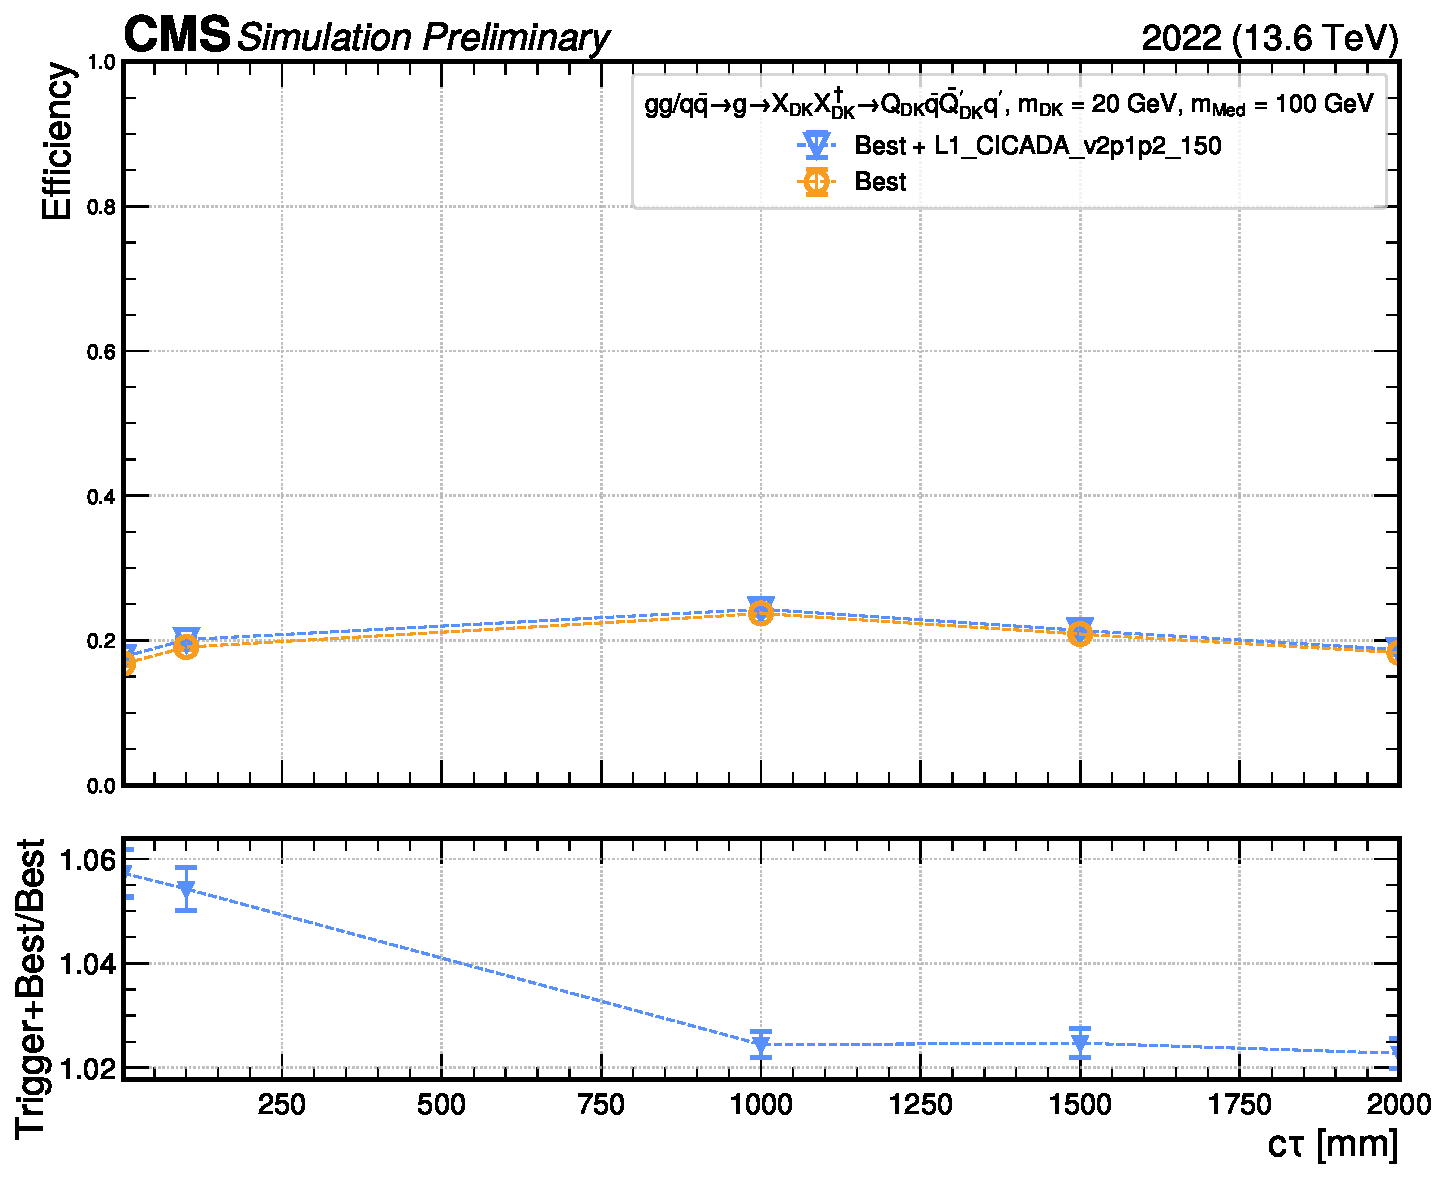
\includegraphics[width=\linewidth]{images/L1/ad_1D_tchan/trigeffplots1D_L1_efftype-trigplusbest_t-channel_mDark-20_mMed-100_L1_CICADA_v2p1p2_150_study_cloppear.pdf}
    \caption{Bifundamental mediator model: Trigger+best object efficiency vs.\ $c\tau$ at $m_\mathrm{med} = 100$ GeV (peak improvement)}
    \label{fig:cicada_eff1D_tchan}
  \end{subfigure}
  \hfill
  % Z' mediator model (s-channel)
  \begin{subfigure}[t]{0.45\textwidth}
    \centering
    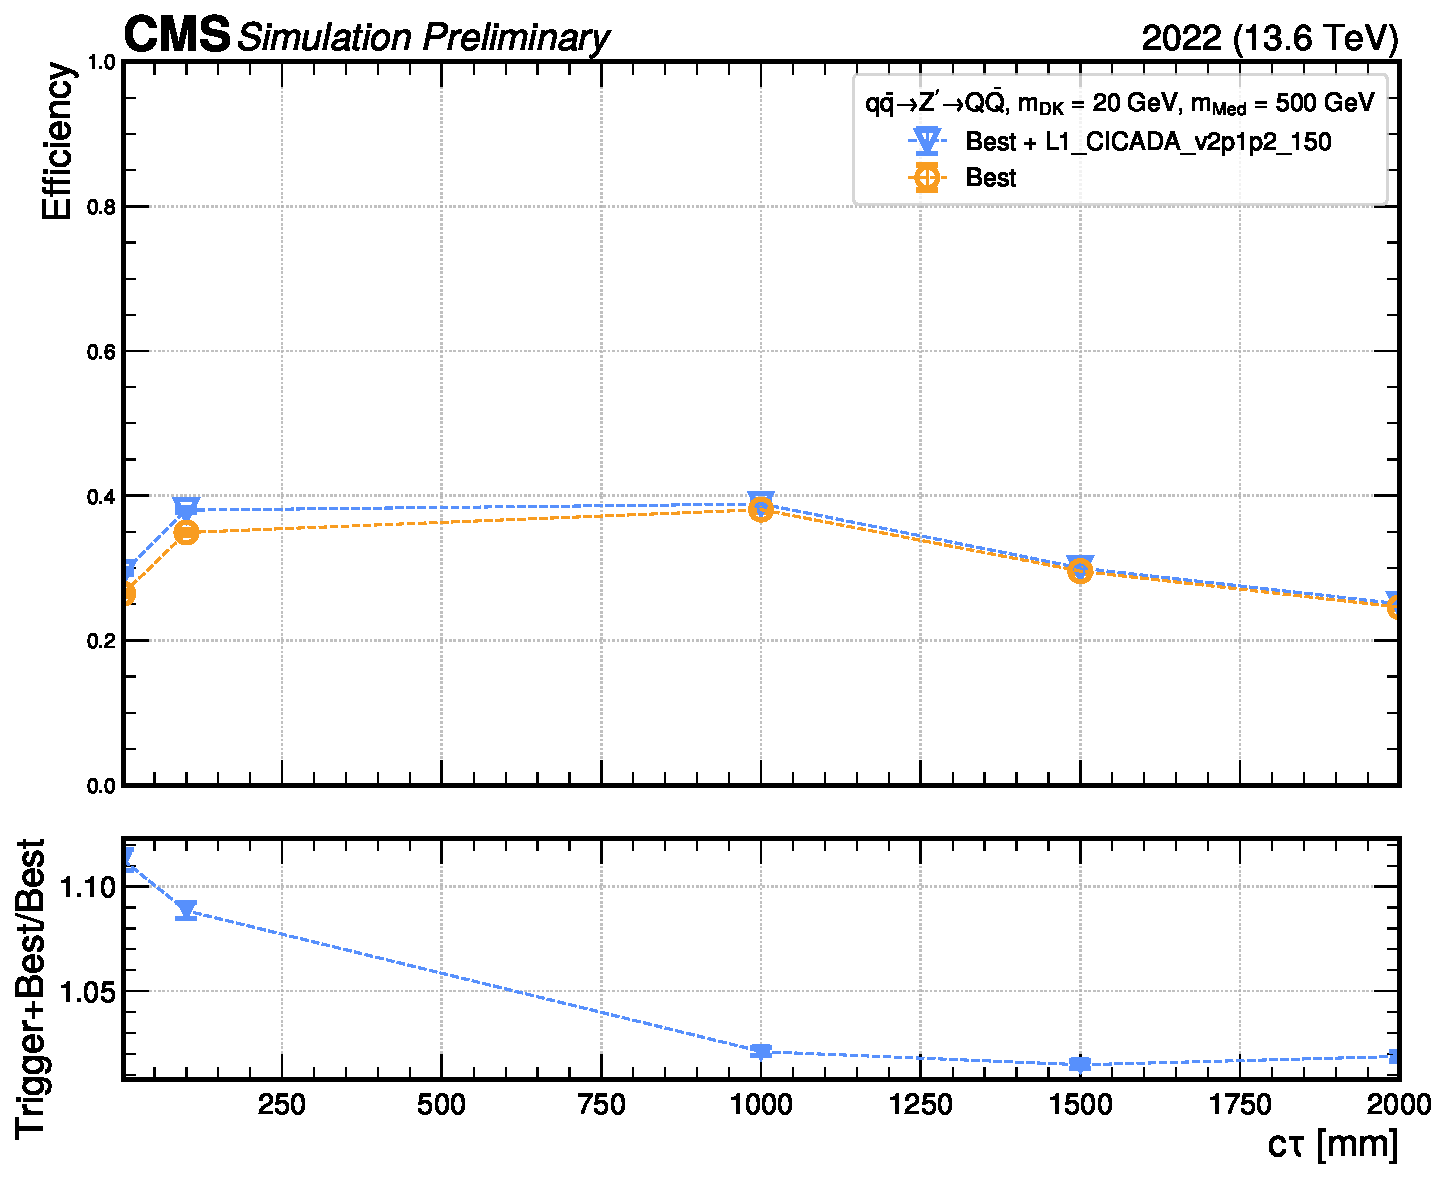
\includegraphics[width=\linewidth]{images/L1/ad_1D_schan/trigeffplots1D_L1_efftype-trigplusbest_s-channel_mDark-20_mMed-500_L1_CICADA_v2p1p2_150_study_cloppear.pdf}
    \caption{Z' mediator model: Trigger+best object efficiency vs.\ $c\tau$ at $m_\mathrm{med} = 500$ GeV (peak improvement)}
    \label{fig:cicada_eff1D_schan}
  \end{subfigure}

  \caption{Trigger+best efficiency as a function of dark pion lifetime $c\tau$ using CICADA, for $m_\mathrm{dark} = 20$ GeV. Each curve corresponds to the mediator mass that yielded the maximum improvement in efficiency for the respective model.}
  \label{fig:cicada_eff1D}
\end{figure}


\begin{figure}[h]
  \centering

  % Trigger-only
  \begin{subfigure}[t]{0.45\textwidth}
    \centering
    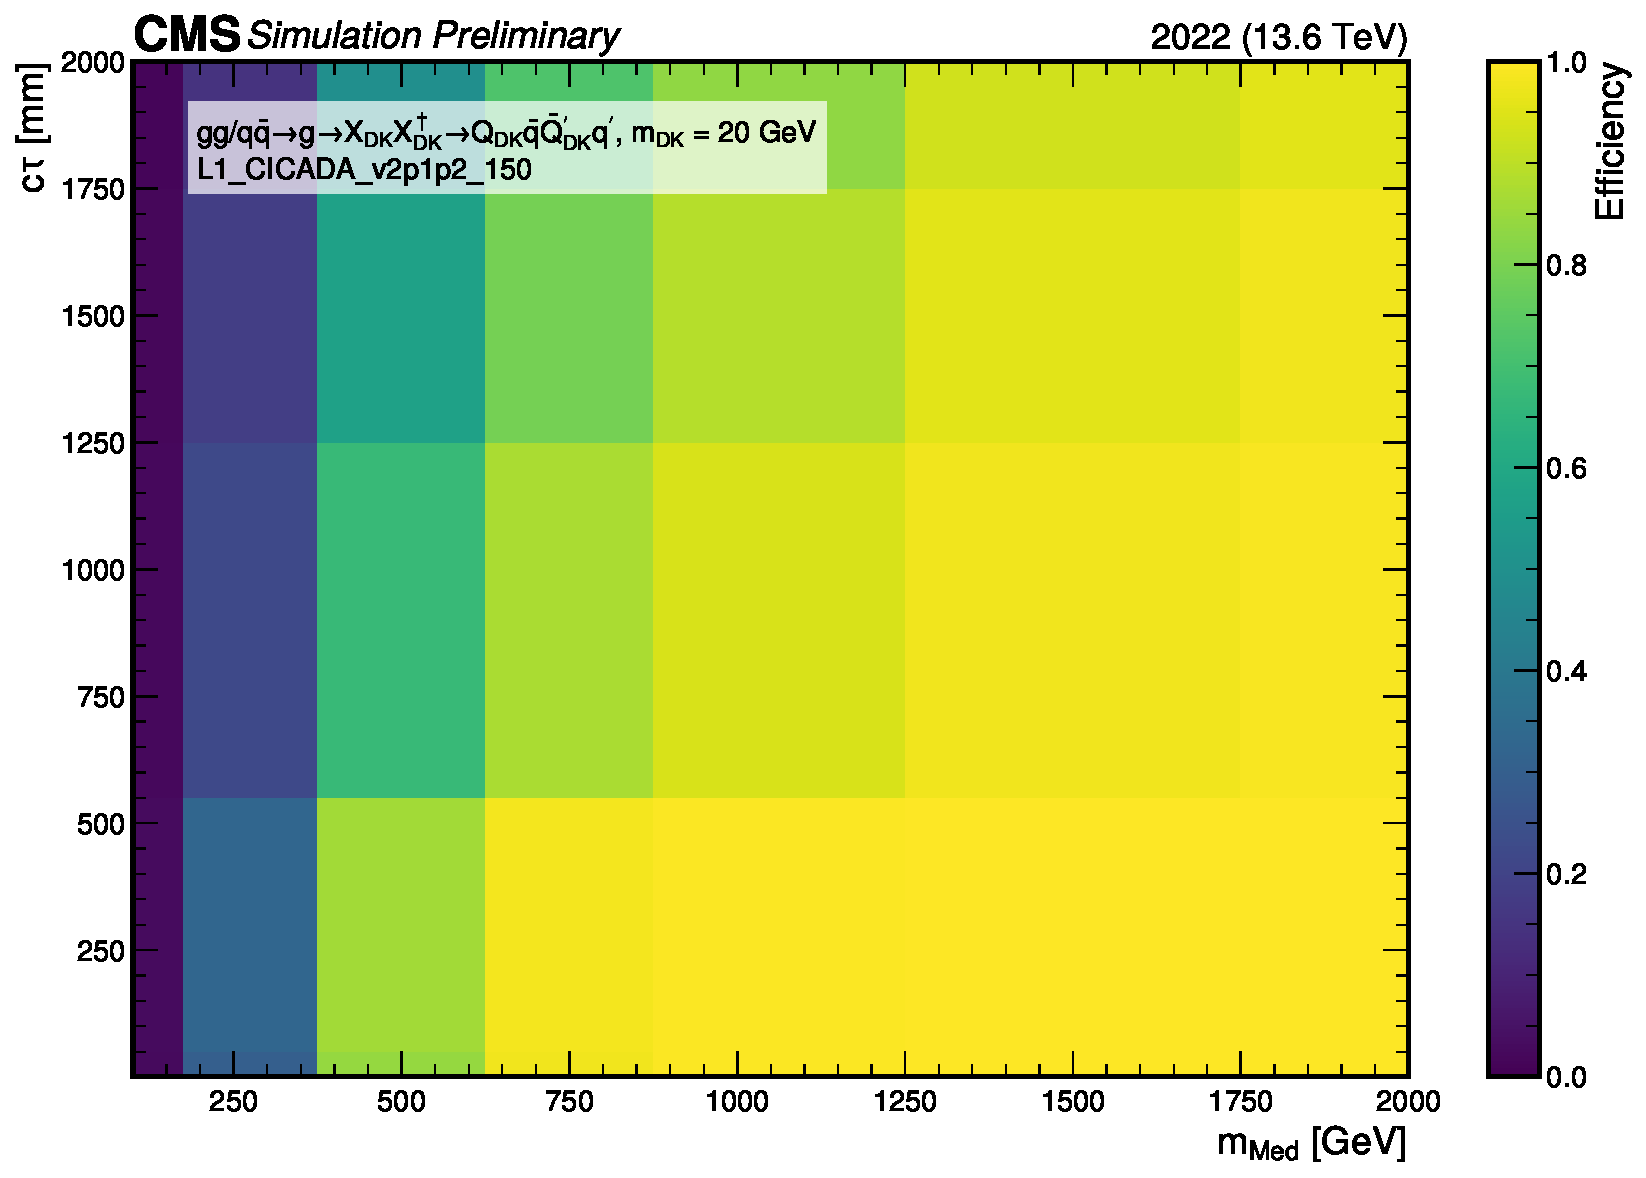
\includegraphics[width=\linewidth]{images/L1/ad_2D_tchan/trigeffplots2D_L1_efftype-trig_t-channel_mDark-20_L1_CICADA_v2p1p2_150_study_cloppear.pdf}
    \caption{Trigger-only, Bifundamental mediator model}
    \label{fig:cicada_trig_tchan}
  \end{subfigure}
  \hfill
  \begin{subfigure}[t]{0.45\textwidth}
    \centering
    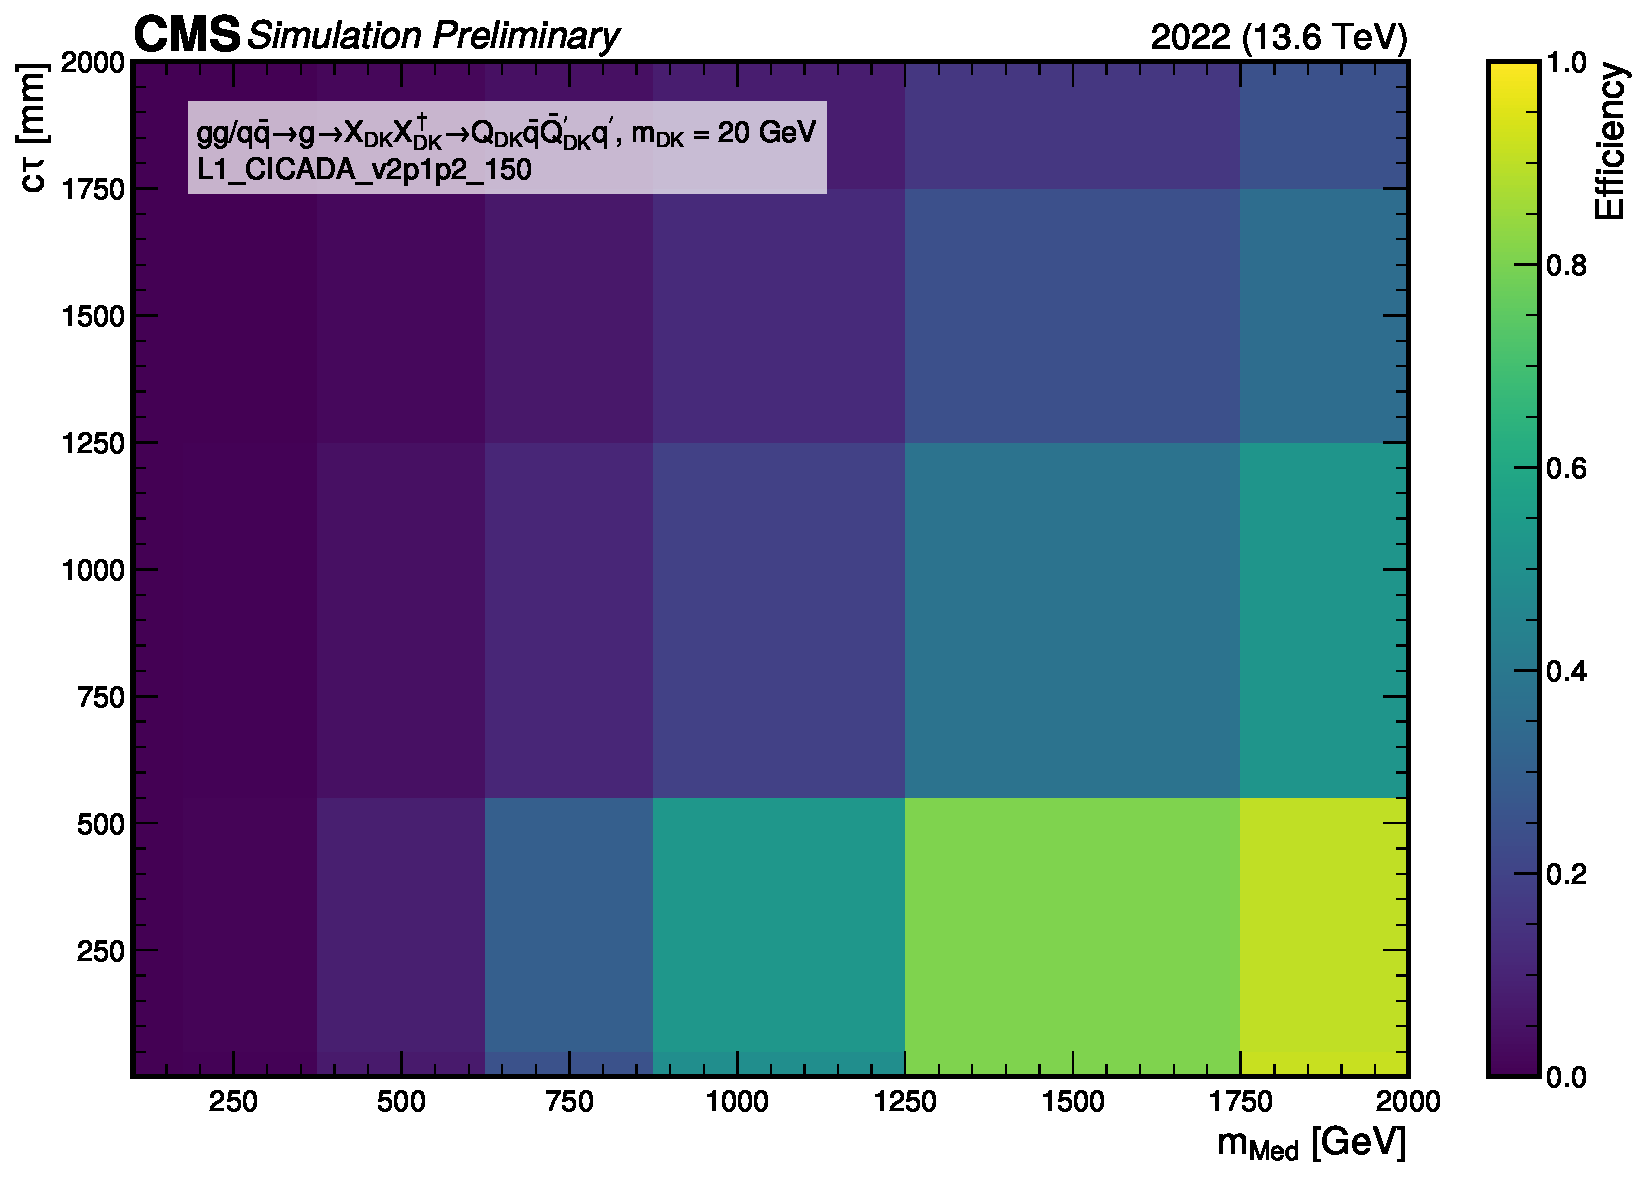
\includegraphics[width=\linewidth]{images/L1/ad_2D_schan/trigeffplots2D_L1_efftype-trig_s-channel_mDark-20_L1_CICADA_v2p1p2_150_study_cloppear.pdf}
    \caption{Trigger-only, Z' mediator model}
    \label{fig:cicada_trig_schan}
  \end{subfigure}

  \vspace{1em}

  % Trigger+best
  \begin{subfigure}[t]{0.45\textwidth}
    \centering
    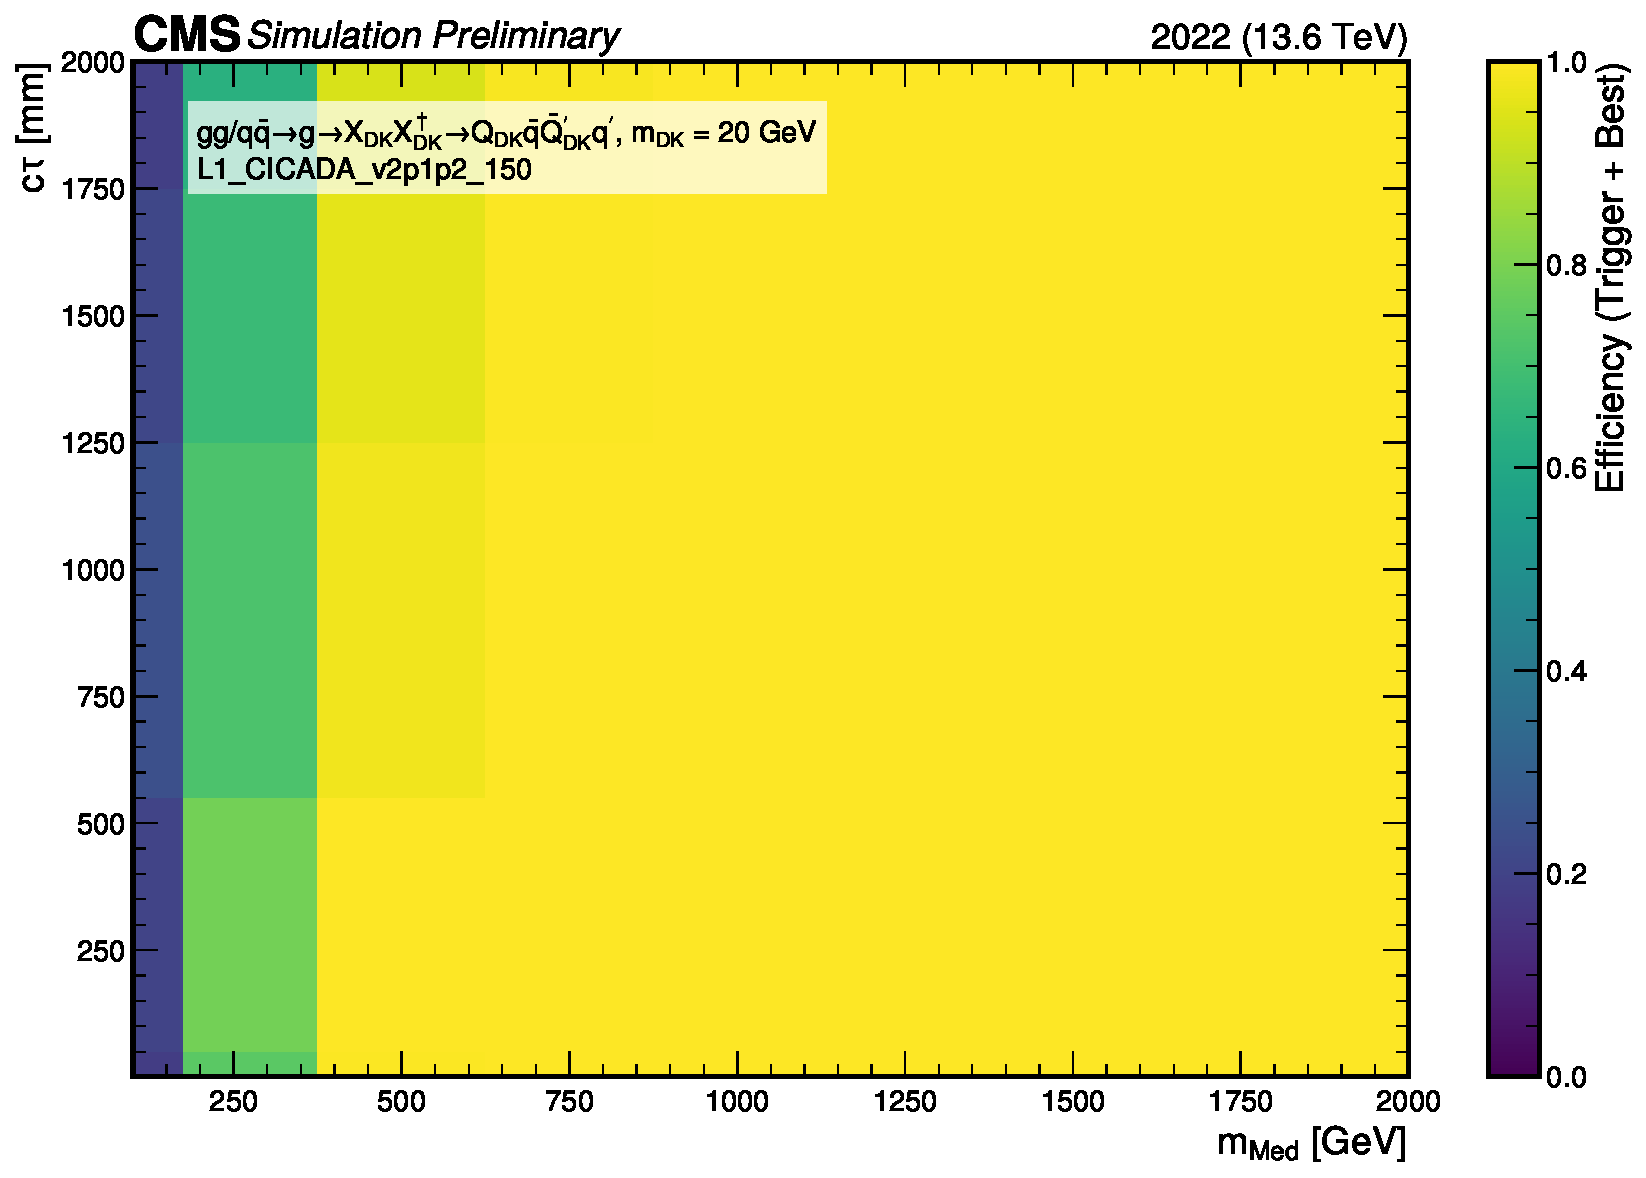
\includegraphics[width=\linewidth]{images/L1/ad_2D_tchan/trigeffplots2D_L1_efftype-trigplusbest_t-channel_mDark-20_L1_CICADA_v2p1p2_150_study_cloppear.pdf}
    \caption{Trigger+best, Bifundamental mediator model}
    \label{fig:cicada_trigplusbest_tchan}
  \end{subfigure}
  \hfill
  \begin{subfigure}[t]{0.45\textwidth}
    \centering
    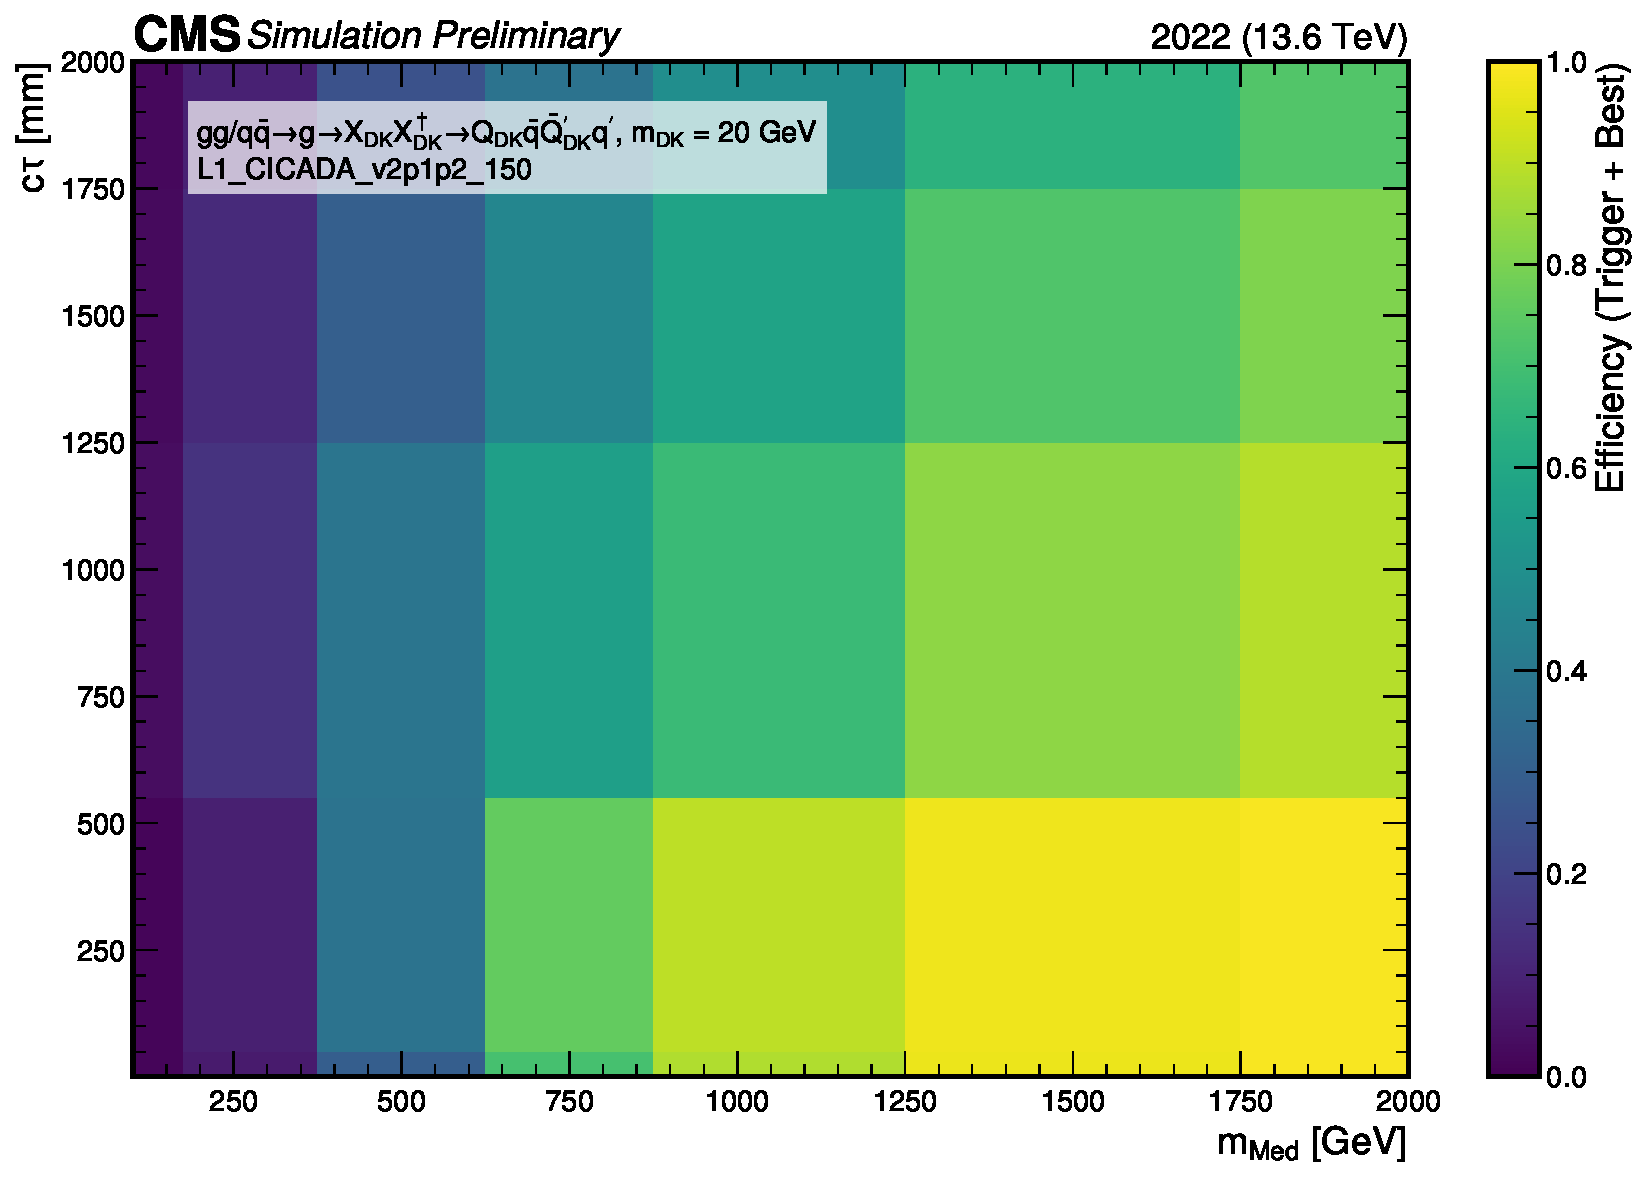
\includegraphics[width=\linewidth]{images/L1/ad_2D_schan/trigeffplots2D_L1_efftype-trigplusbest_s-channel_mDark-20_L1_CICADA_v2p1p2_150_study_cloppear.pdf}
    \caption{Trigger+best, Z' mediator model}
    \label{fig:cicada_trigplusbest_schan}
  \end{subfigure}

  \vspace{1em}

  % Improvement
  \begin{subfigure}[t]{0.45\textwidth}
    \centering
    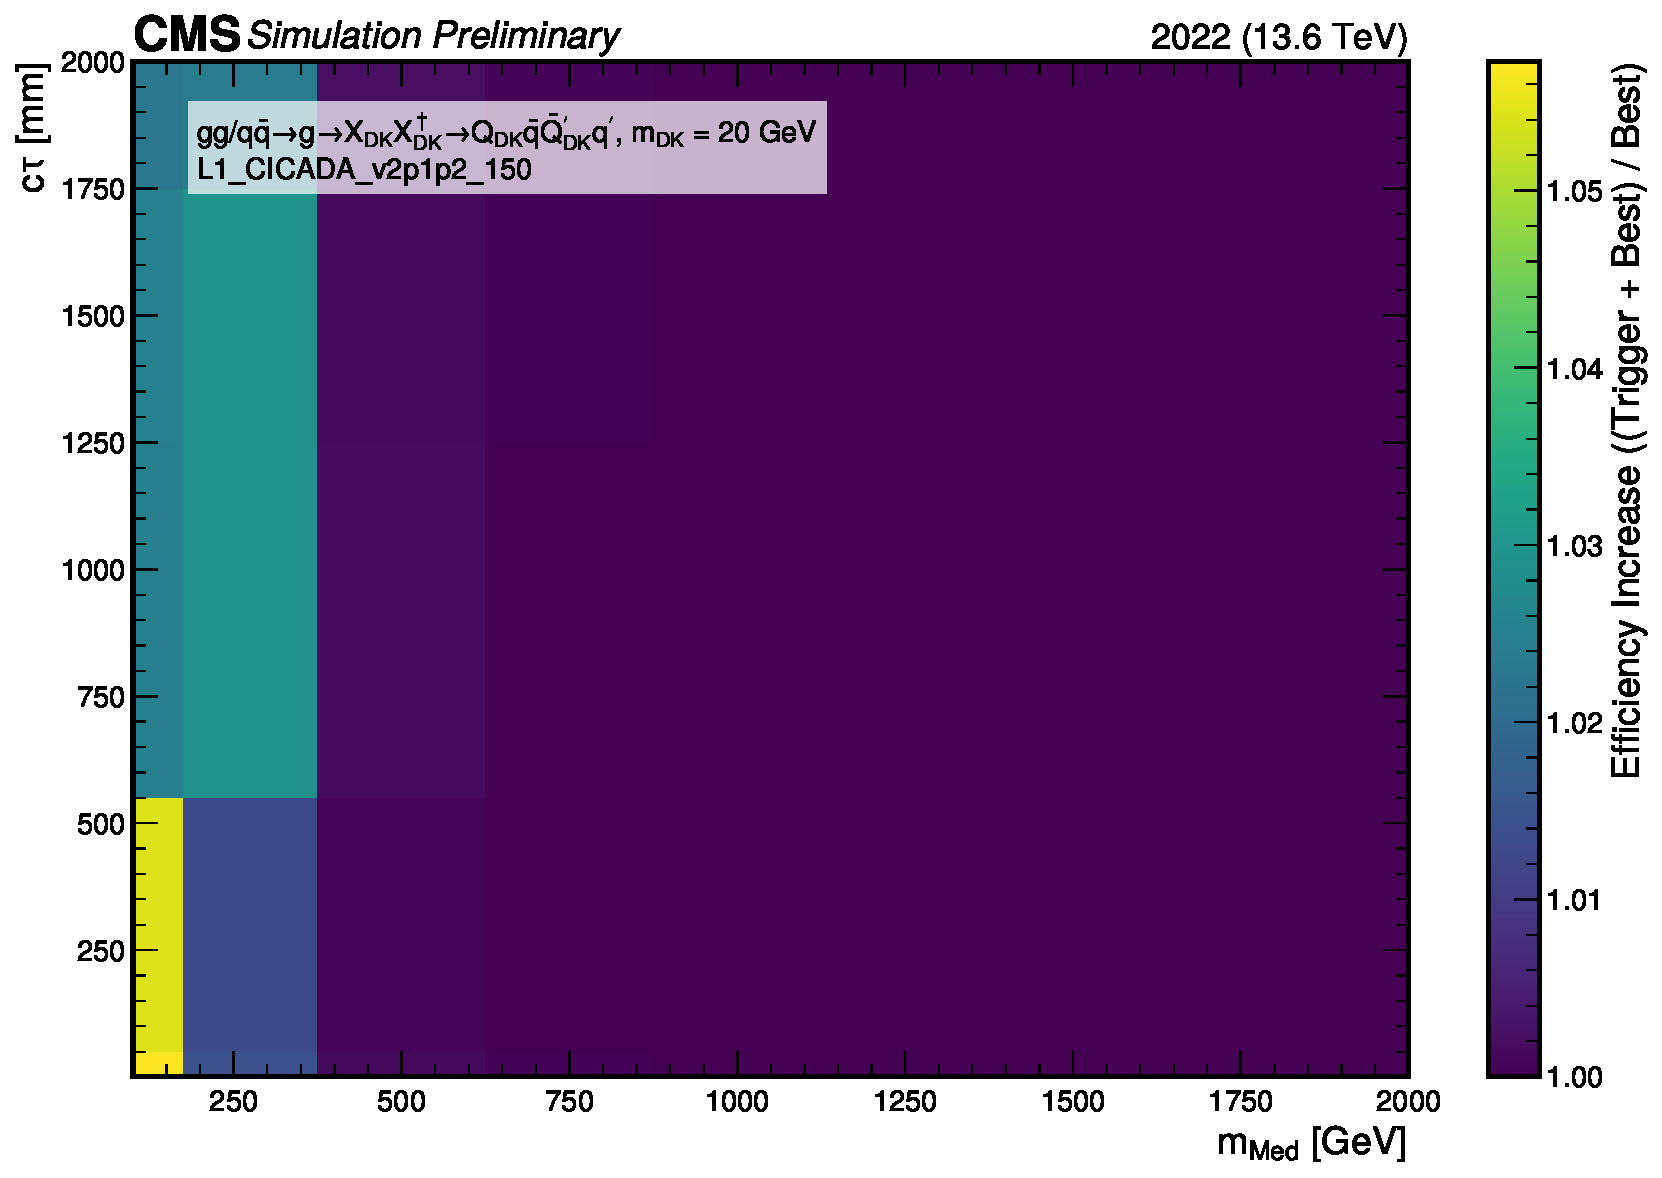
\includegraphics[width=\linewidth]{images/L1/ad_2D_tchan/trigeffplots2D_L1_efftype-improv_t-channel_mDark-20_L1_CICADA_v2p1p2_150_study_cloppear.pdf}
    \caption{Improvement, Bifundamental mediator model}
    \label{fig:cicada_improv_tchan}
  \end{subfigure}
  \hfill
  \begin{subfigure}[t]{0.45\textwidth}
    \centering
    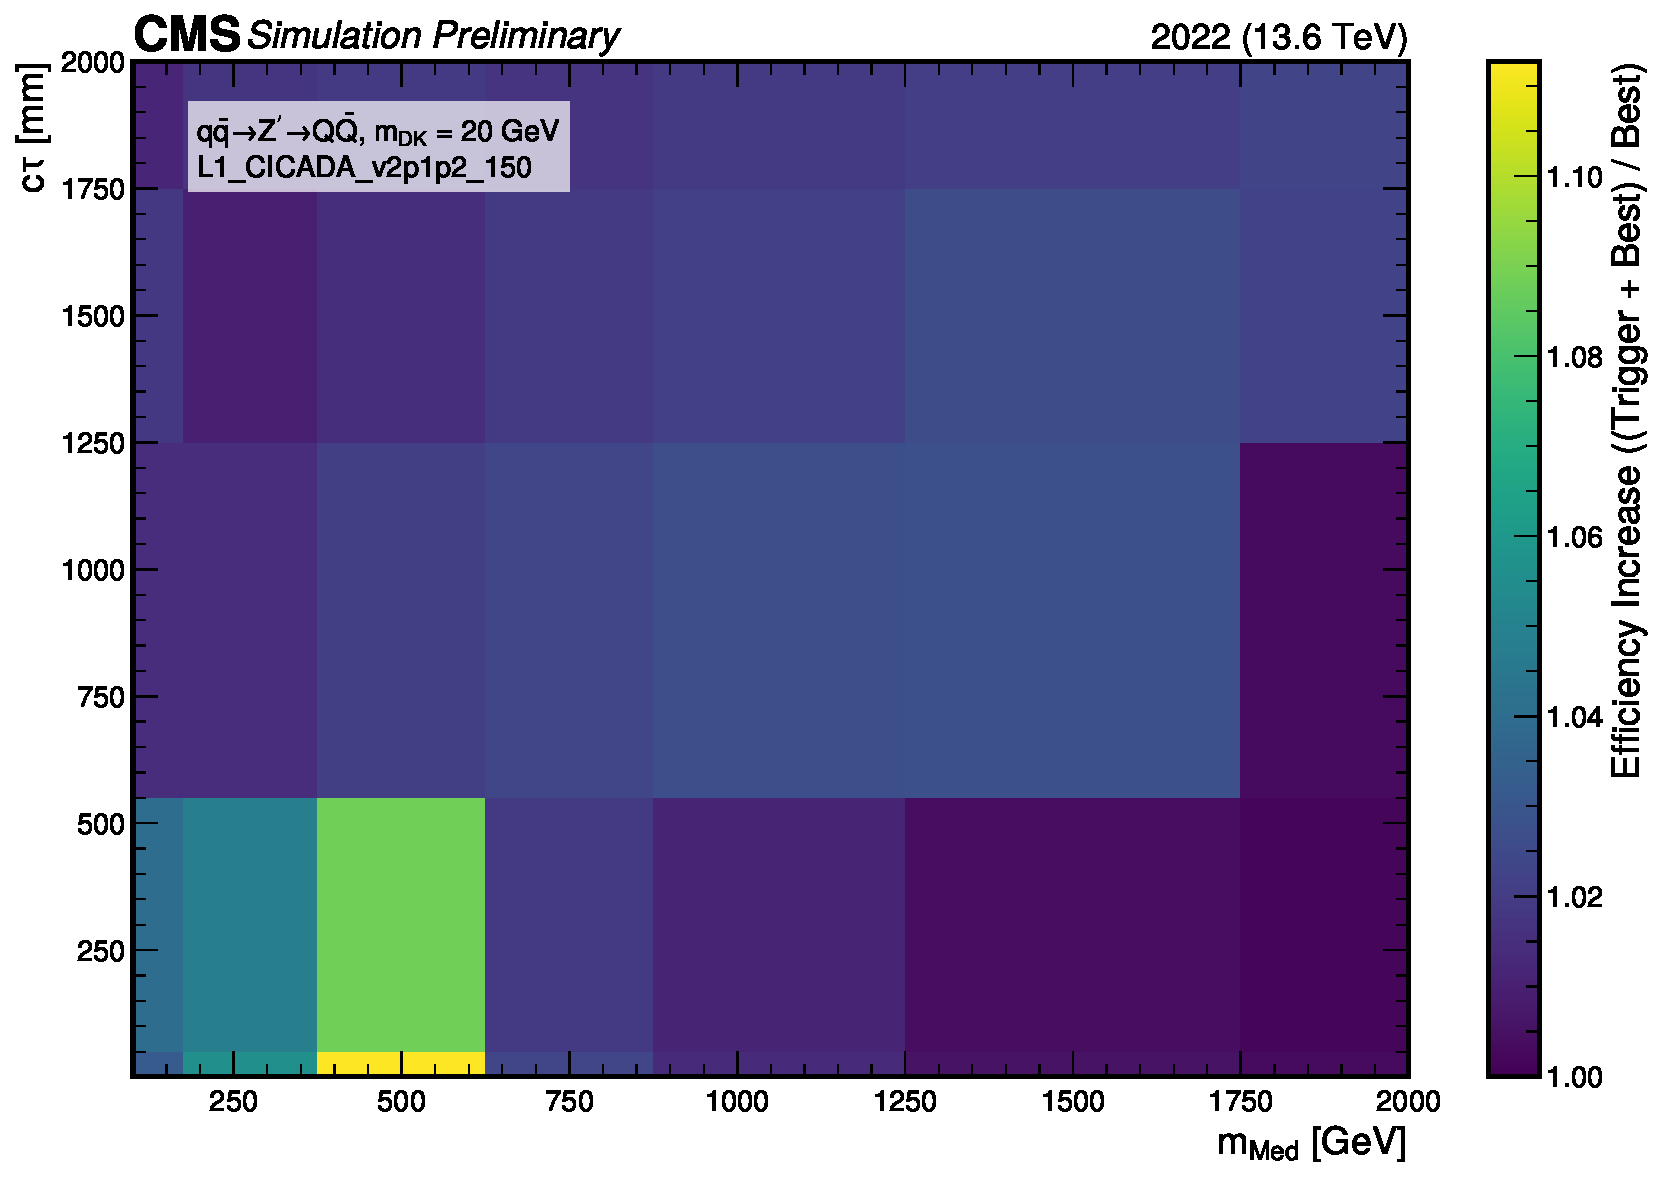
\includegraphics[width=\linewidth]{images/L1/ad_2D_schan/trigeffplots2D_L1_efftype-improv_s-channel_mDark-20_L1_CICADA_v2p1p2_150_study_cloppear.pdf}
    \caption{Improvement, Z' mediator model}
    \label{fig:cicada_improv_schan}
  \end{subfigure}

  \caption{CICADA trigger efficiency heatmaps for $m_\mathrm{dark} = 20$ GeV in both the bifundamental mediator model and the Z' mediator model.}
  \label{fig:cicada_eff}
\end{figure}

%-------%-------%-------%-------%-------%-------%-------%-------%-------%-------%-------%-------

% While triggers targeting particular expected signatures produced by physics beyond the Standard Model are effective, they become a limitation when there is no strong theoretical prior. It was under this consideration that AD triggers were developed, with the goal of increasing sensitivity to signals for which there are no dedicated signatures. These triggers utilize unsupervised ML techniques to search for new physics signatures. However, because the resources available at the level-1 trigger system are heavily restricted, as described in \ref{govorkovaAutoencodersFPGAsRealtime2022}, multiple techniques, such as knowledge distillation and quantum aware training (QAT), are implemented in order to allow these models to fit in FPGAs which can then be deployed.

% The two AD triggers considered in these studies are AXOL1TL, based on a variational autoencoder, and CICADA, based on a convolutional autoencoder. The models these triggers use are trained on an unbiased random sample of events, most of which correspond to known physics or where there was little momentum transfer. AXOL1TL uses as its input the $p_T$, $\eta$, and $\phi$ of 18 level-1 reconstructed objects, namely 4 muons, 4 electrons, and 10 jets, as well as the magnitude and $\phi$ coordinate of the event's level-1 reconstruction of the MET. The loss function used during training is:

% \begin{equation}
%     \mathcal{L_\text{AXO}} = (1-\beta)\text{MSE(Output, Input)} + \beta\text{D}_{\text{KL}}(\vec \mu, \vec \sigma)
%     \label{}
% \end{equation}

% where $\text{D}_{\text{KL}}$ is the Kullback-Leibler regularization term, and $\beta\in [0,1]$ is a hyperparameter used to adjust the optimization priority of the two terms in the loss function. The deployed trigger, however, only uses the encoder section of the model, and it outputs the mean in the latent space of the quantized model as the 



% CICADA, on the other hand, uses the calorimeter region energies. Note, however, that what is actually deployed in the FPGAs are not the full trained models, but rather a reduced version of them which 

\section{Long-Lived Particle Triggers}

The Phase-1 upgrade to CMS introduced precision timing information and depth segmentation to the HCAL barrel and endcap. This enabled the introduction of these sets of triggers which take advantage of this information in order to specifically target the longer-lived regime of the parameter space of many models with long-lived particles. In particular, they selected events with jets displaced with respect to the primary vertex and jets delayed significantly with respect to the bunch crossing. The displaced jet triggers select events in which there are HCAL trigger towers with lower energy in the lower depths, but higher in the more exterior ones. The delayed jet triggers, on the other hand, flag events with pulses arriving late. Note that because these last triggers search for very slowly decaying LLPs (i.e., decaying in between bunch crossings), they were not included in this study. The muon system high multiplicity trigger is another type of LLP trigger which was studied. However, this trigger selects events with a high number of localized hits in the Cathode Strip Chamber (CSC) in the muon detector, serving as an extra handle for the search for EMJs for models with very high lifetimes.

The efficiencies of the two previously mentioned types of triggers were studied. The trigger efficiency heat maps of the first of these triggers, \texttt{L1\_HTT200\_SingleLLPJet60}, can be seen in Figures \ref{fig:htt200singlellpjet60_trig_tchan} and \ref{fig:htt200singlellpjet60_trig_schan} for both the bifundamental model and the $Z'$ model. From these plots, we can clearly see that this trigger targets the longer-lived regime, peaking for samples from both mediator models with $c\tau_{\text{dark}} = 1000 \text{ GeV}$. This behavior was expected, given that the sub-jets produced from dark pions decaying back into SM particles in and around the HCAL would have a high likelihood of resulting in the event being flagged as having an LLP jet. 

A very promising observation from these results can be seen in the efficiency improvement plots seen in Figures \ref{fig:htt200singlellpjet60_improv_tchan} and \ref{fig:htt200singlellpjet60_improv_schan}. These show that the highest efficiency gain is exactly in those regions of the parameter space for which even the best conventional triggers have low efficiency. Unfortunately, this $\text{EI}$ is relatively low. A very similar increase in sensitivity is seen for \texttt{L1\_DoubleLLPJet40} (Figures \ref{fig:htt200singlellpjet60_improv_tchan} and \ref{fig:htt200singlellpjet60_improv_schan}); this trigger offers a peak in increased sensitivity for high $c\tau_{\text{dark}}$ and low $m_{\text{Med}}$. However, in both mediator models the increase in efficiency is $<2\%$, lower than that of \texttt{L1\_HTT200\_SingleLLPJet60}. This result is to be expected, as the requirement for there to be two LLP flagged jets is more stringent than that for there to be one (even if we consider that \texttt{L1\_HTT200\_SingleLLPJet60} has a higher jet energy threshold and the additional requirement of $H_T>200$, which is anyways are likely to be met given the high jet activity characteristic of this type of DS model). This conclusion is supported by the observation that the overall raw efficiency seen in Figures \ref{fig:htt200singlellpjet60_trig_tchan} and \ref{fig:htt200singlellpjet60_trig_schan} is higher than in Figures \ref{fig:doublellp_trig_tchan} and \ref{fig:doublellp_trig_schan}.

\begin{figure}[h]
  \centering

  % Trigger-only
  \begin{subfigure}[t]{0.45\textwidth}
    \centering
    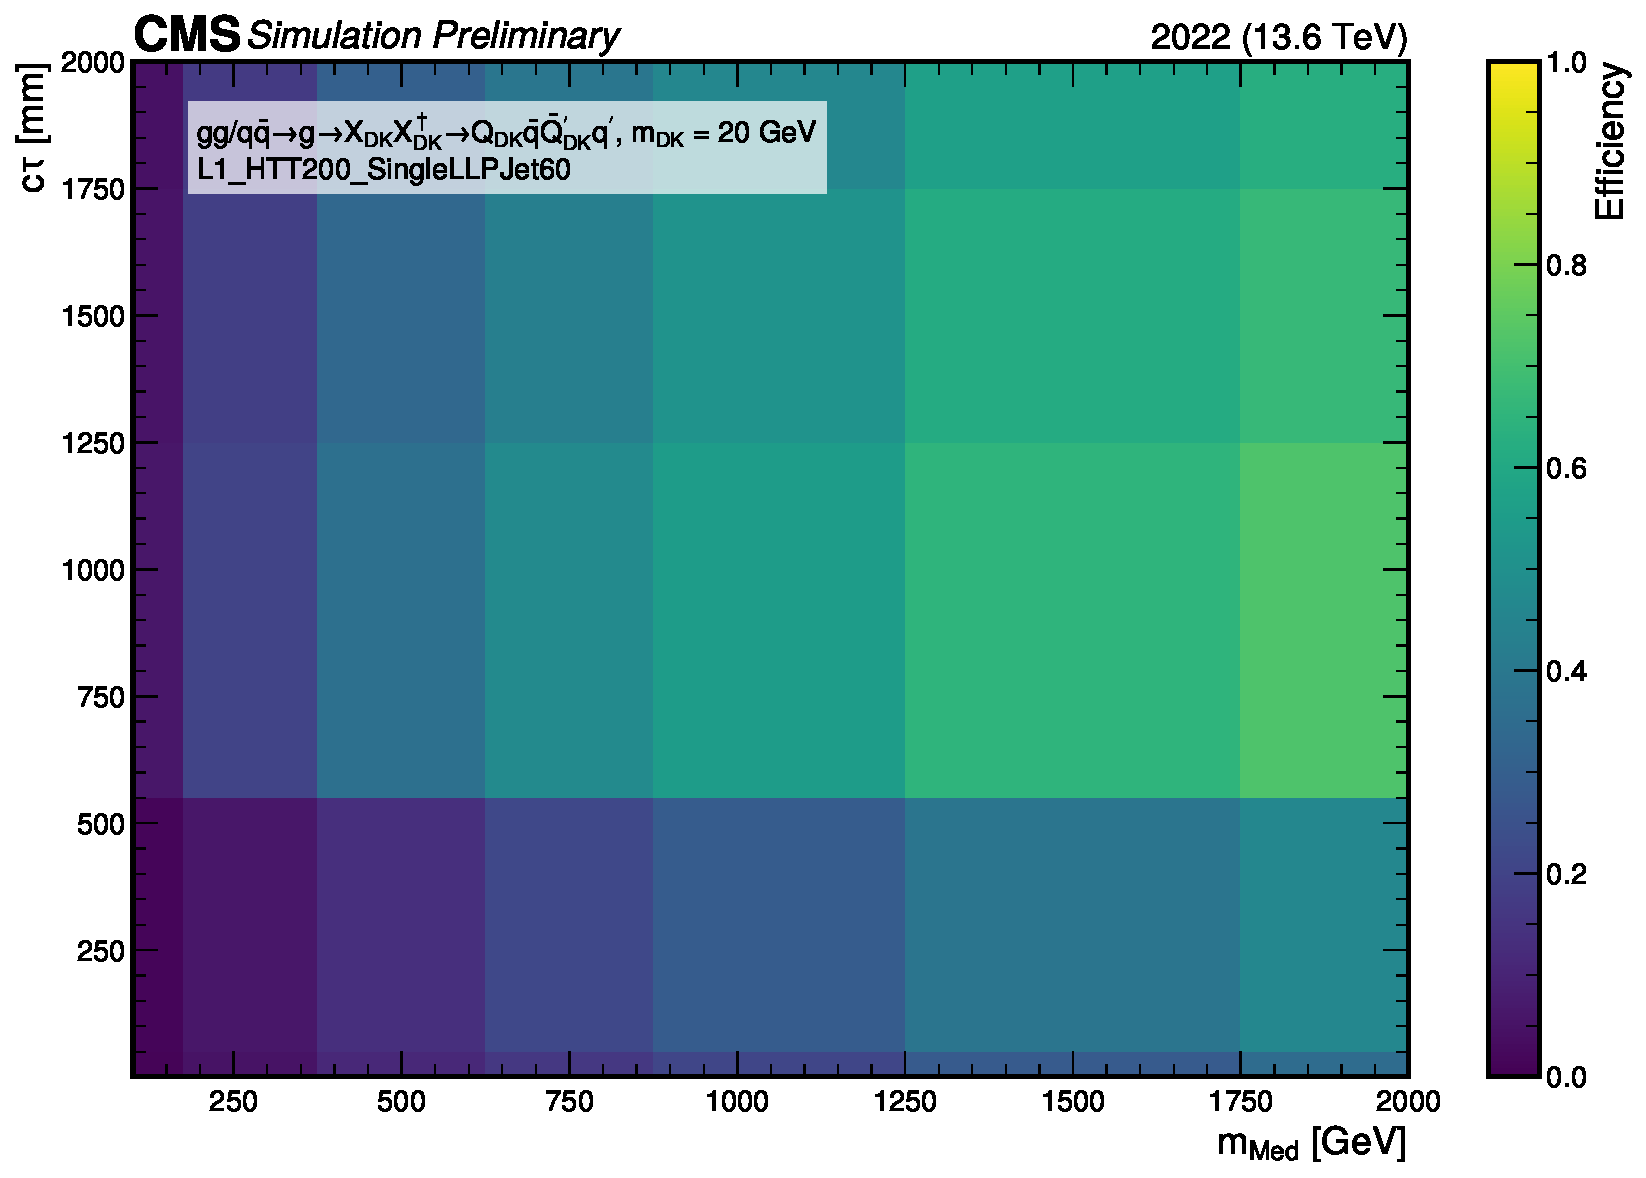
\includegraphics[width=\linewidth]{images/L1/llp_2D_tchan/trigeffplots2D_L1_efftype-trig_t-channel_mDark-20_L1_HTT200_SingleLLPJet60_study_cloppear.pdf}
    \caption{Trigger-only, Bifundamental mediator model}
    \label{fig:htt200singlellpjet60_trig_tchan}
  \end{subfigure}
  \hfill
  \begin{subfigure}[t]{0.45\textwidth}
    \centering
    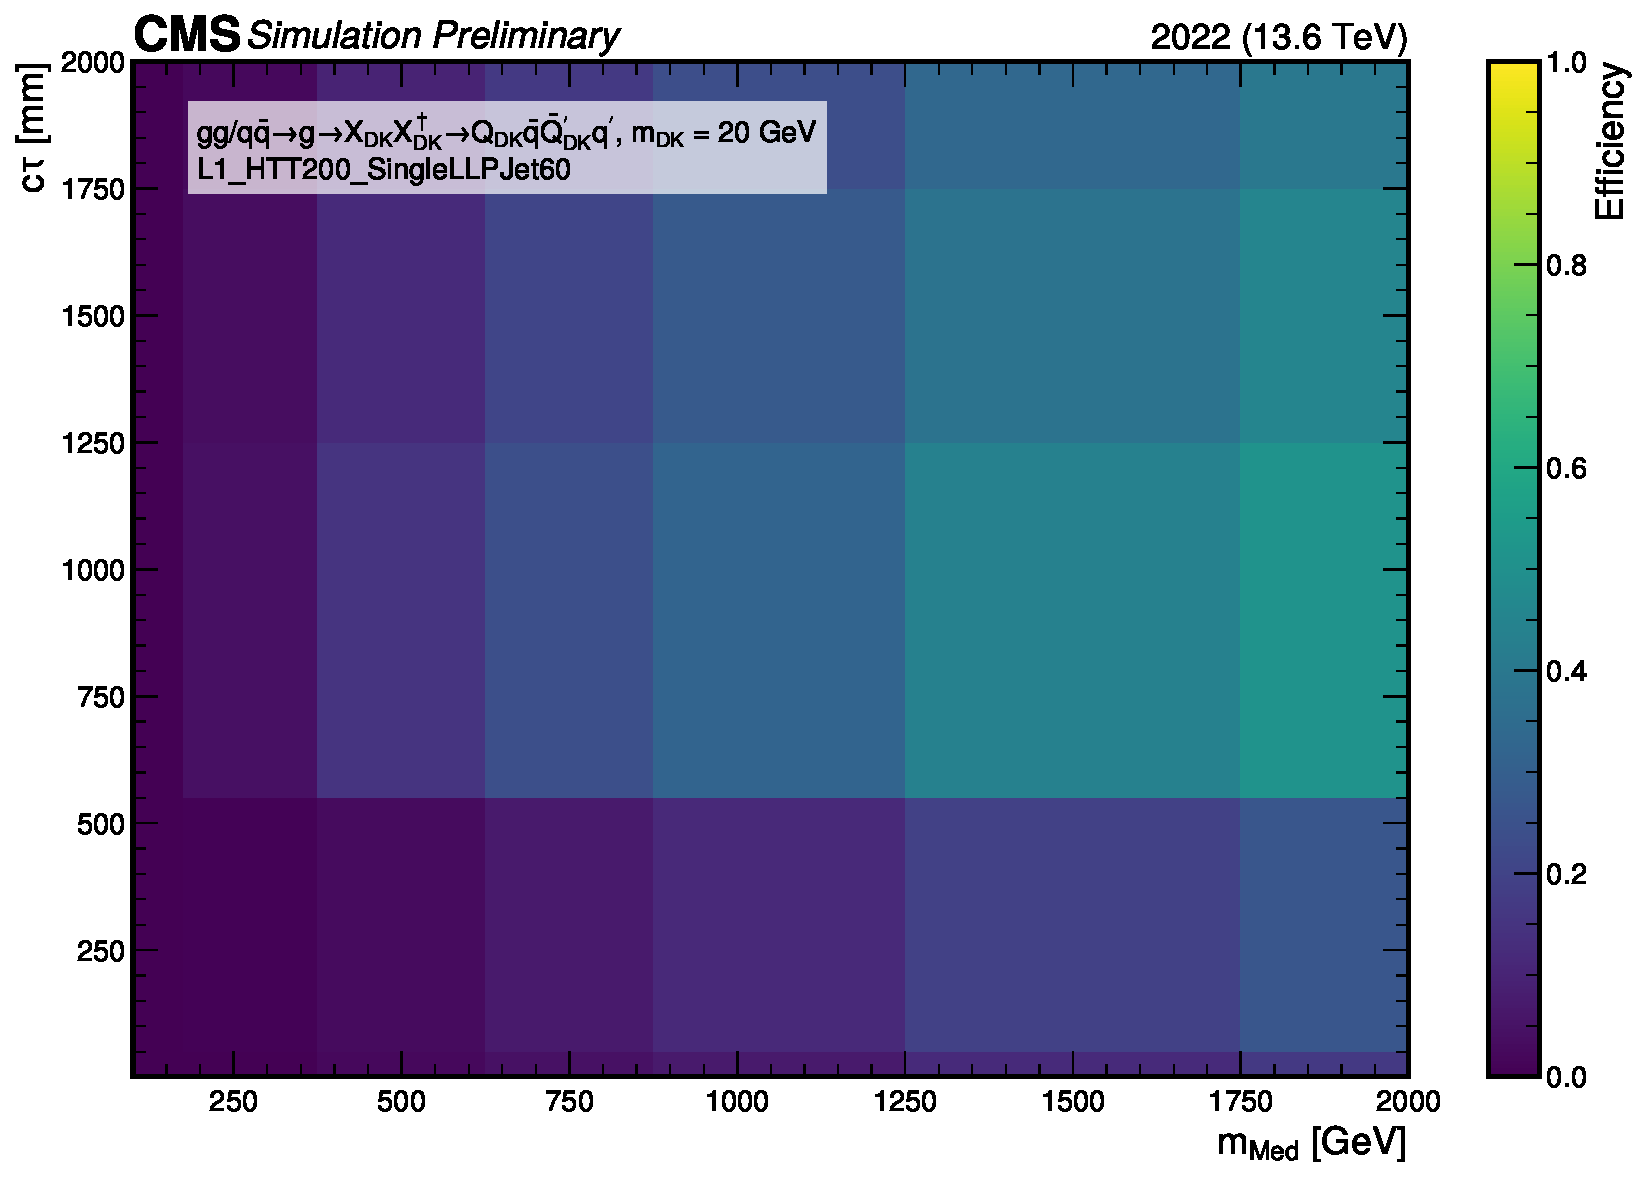
\includegraphics[width=\linewidth]{images/L1/llp_2D_schan/trigeffplots2D_L1_efftype-trig_s-channel_mDark-20_L1_HTT200_SingleLLPJet60_study_cloppear.pdf}
    \caption{Trigger-only, Z' mediator model}
    \label{fig:htt200singlellpjet60_trig_schan}
  \end{subfigure}

  \vspace{1em}

  % Trigger+best
  \begin{subfigure}[t]{0.45\textwidth}
    \centering
    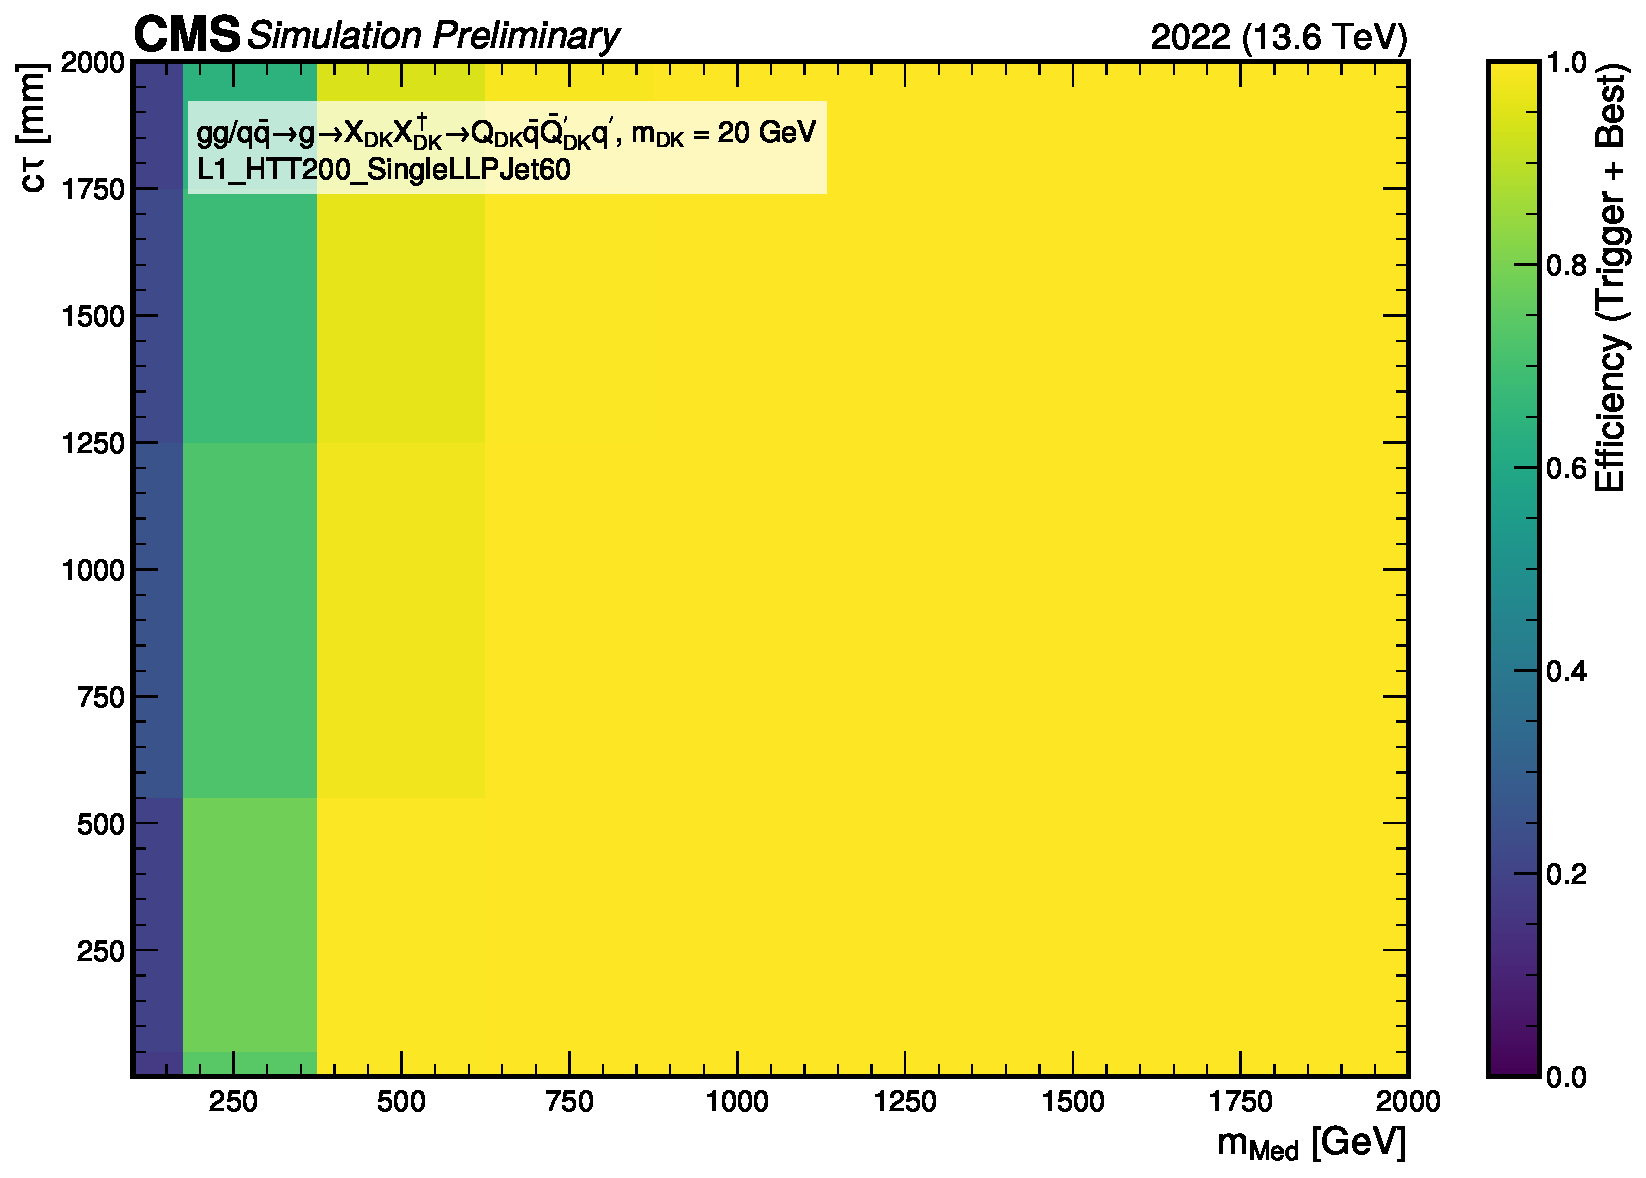
\includegraphics[width=\linewidth]{images/L1/llp_2D_tchan/trigeffplots2D_L1_efftype-trigplusbest_t-channel_mDark-20_L1_HTT200_SingleLLPJet60_study_cloppear.pdf}
    \caption{Trigger+best, Bifundamental mediator model}
    \label{fig:htt200singlellpjet60_trigplusbest_tchan}
  \end{subfigure}
  \hfill
  \begin{subfigure}[t]{0.45\textwidth}
    \centering
    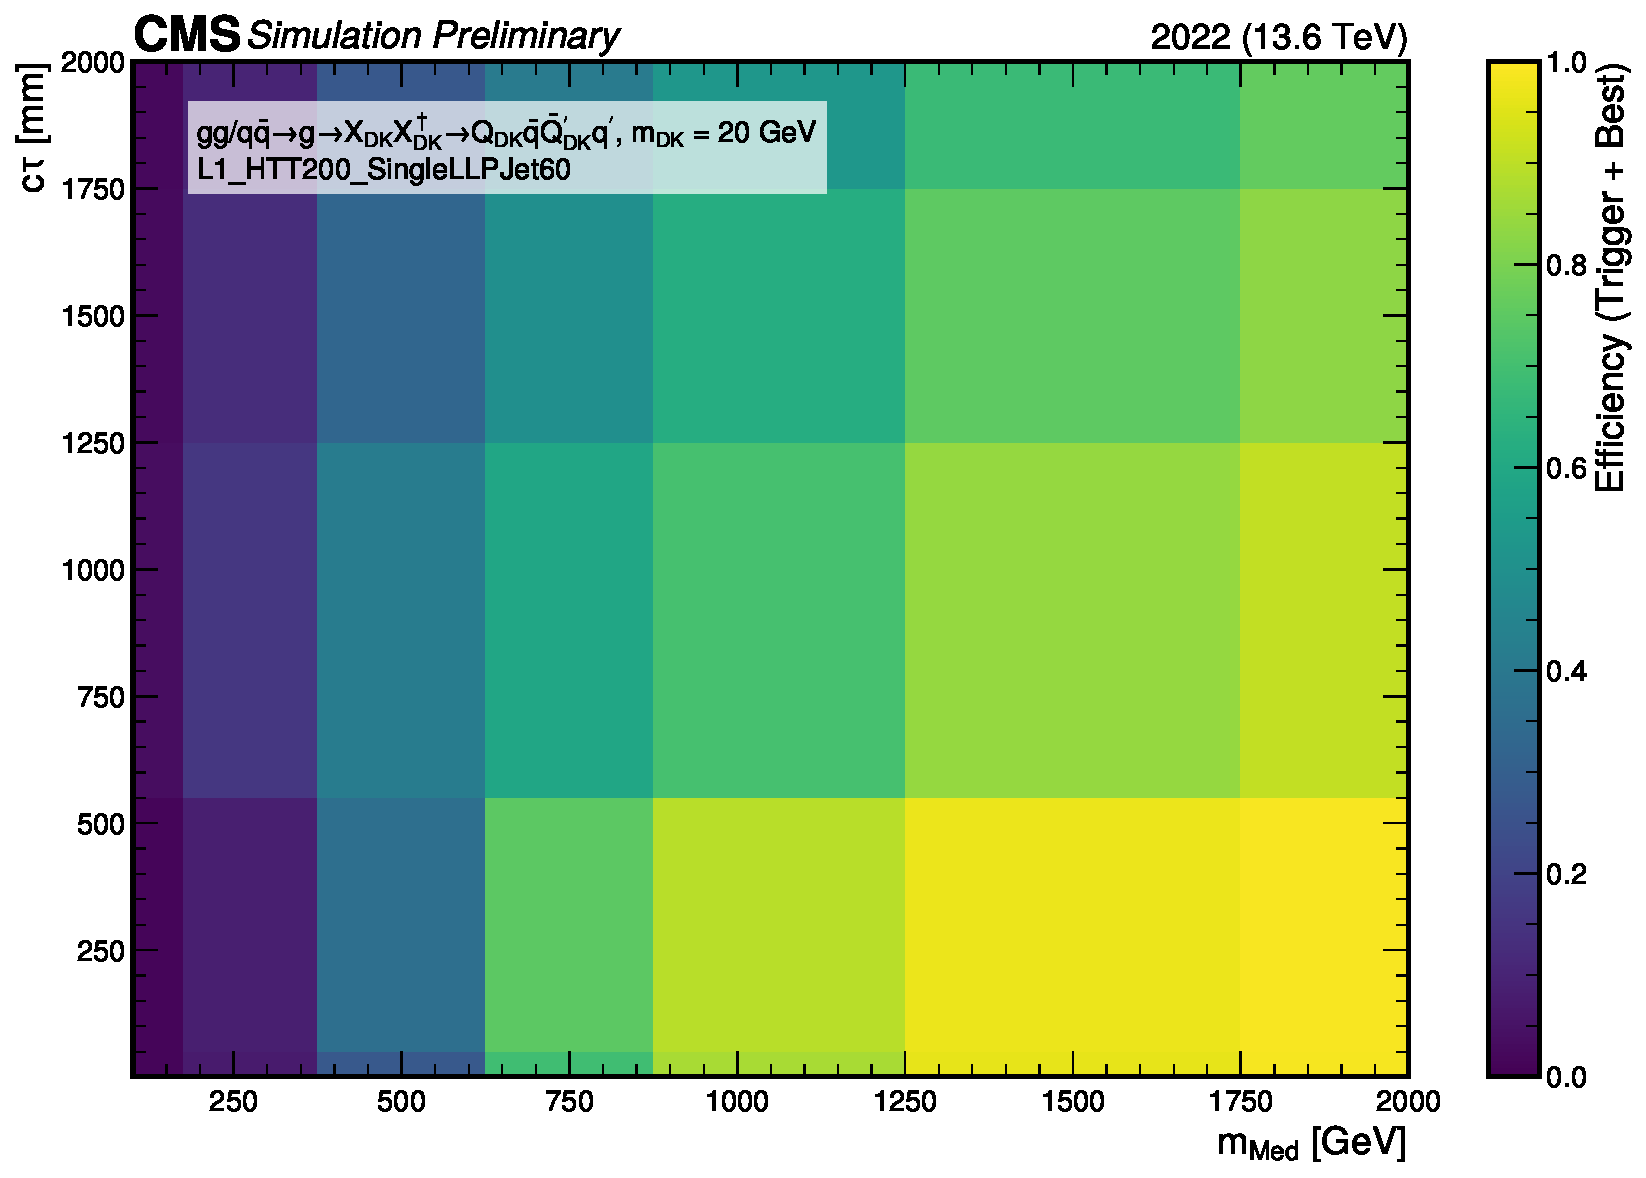
\includegraphics[width=\linewidth]{images/L1/llp_2D_schan/trigeffplots2D_L1_efftype-trigplusbest_s-channel_mDark-20_L1_HTT200_SingleLLPJet60_study_cloppear.pdf}
    \caption{Trigger+best, Z' mediator model}
    \label{fig:htt200singlellpjet60_trigplusbest_schan}
  \end{subfigure}

  \vspace{1em}

  % Improvement
  \begin{subfigure}[t]{0.45\textwidth}
    \centering
    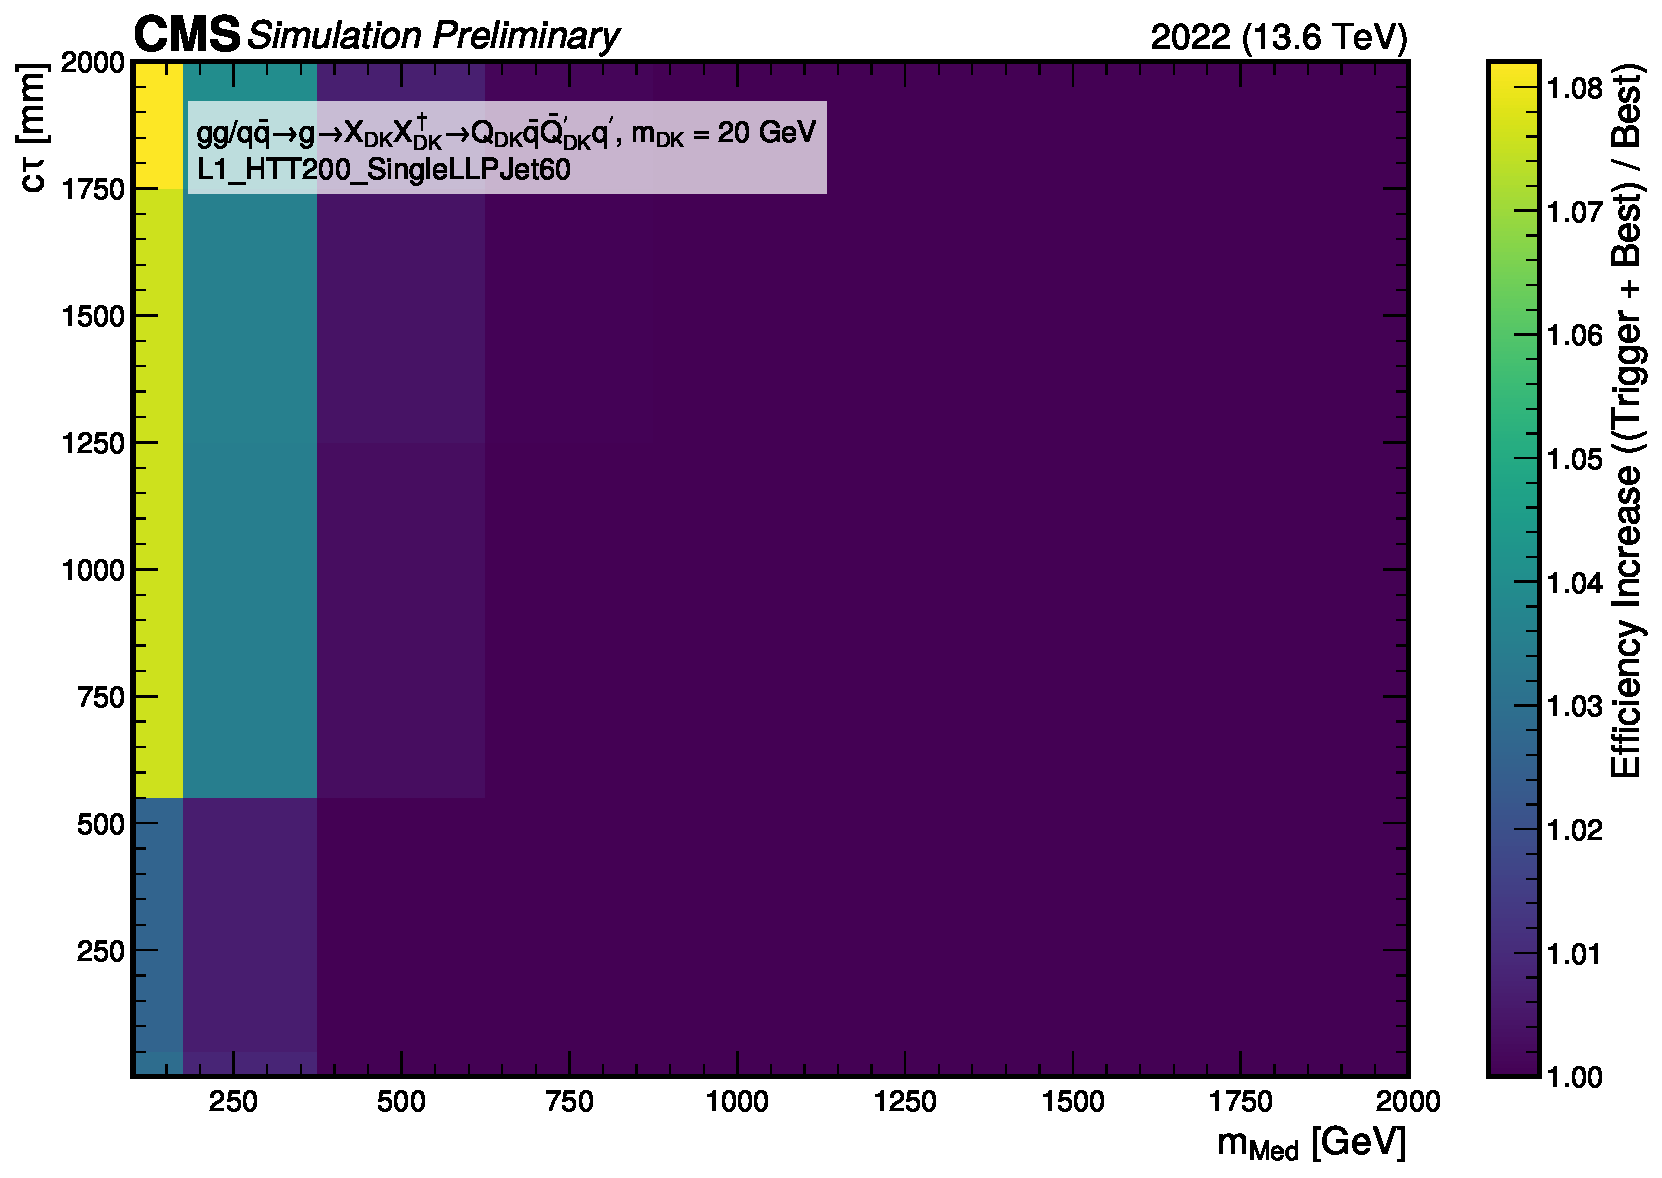
\includegraphics[width=\linewidth]{images/L1/llp_2D_tchan/trigeffplots2D_L1_efftype-improv_t-channel_mDark-20_L1_HTT200_SingleLLPJet60_study_cloppear.pdf}
    \caption{Improvement, Bifundamental mediator model}
    \label{fig:htt200singlellpjet60_improv_tchan}
  \end{subfigure}
  \hfill
  \begin{subfigure}[t]{0.45\textwidth}
    \centering
    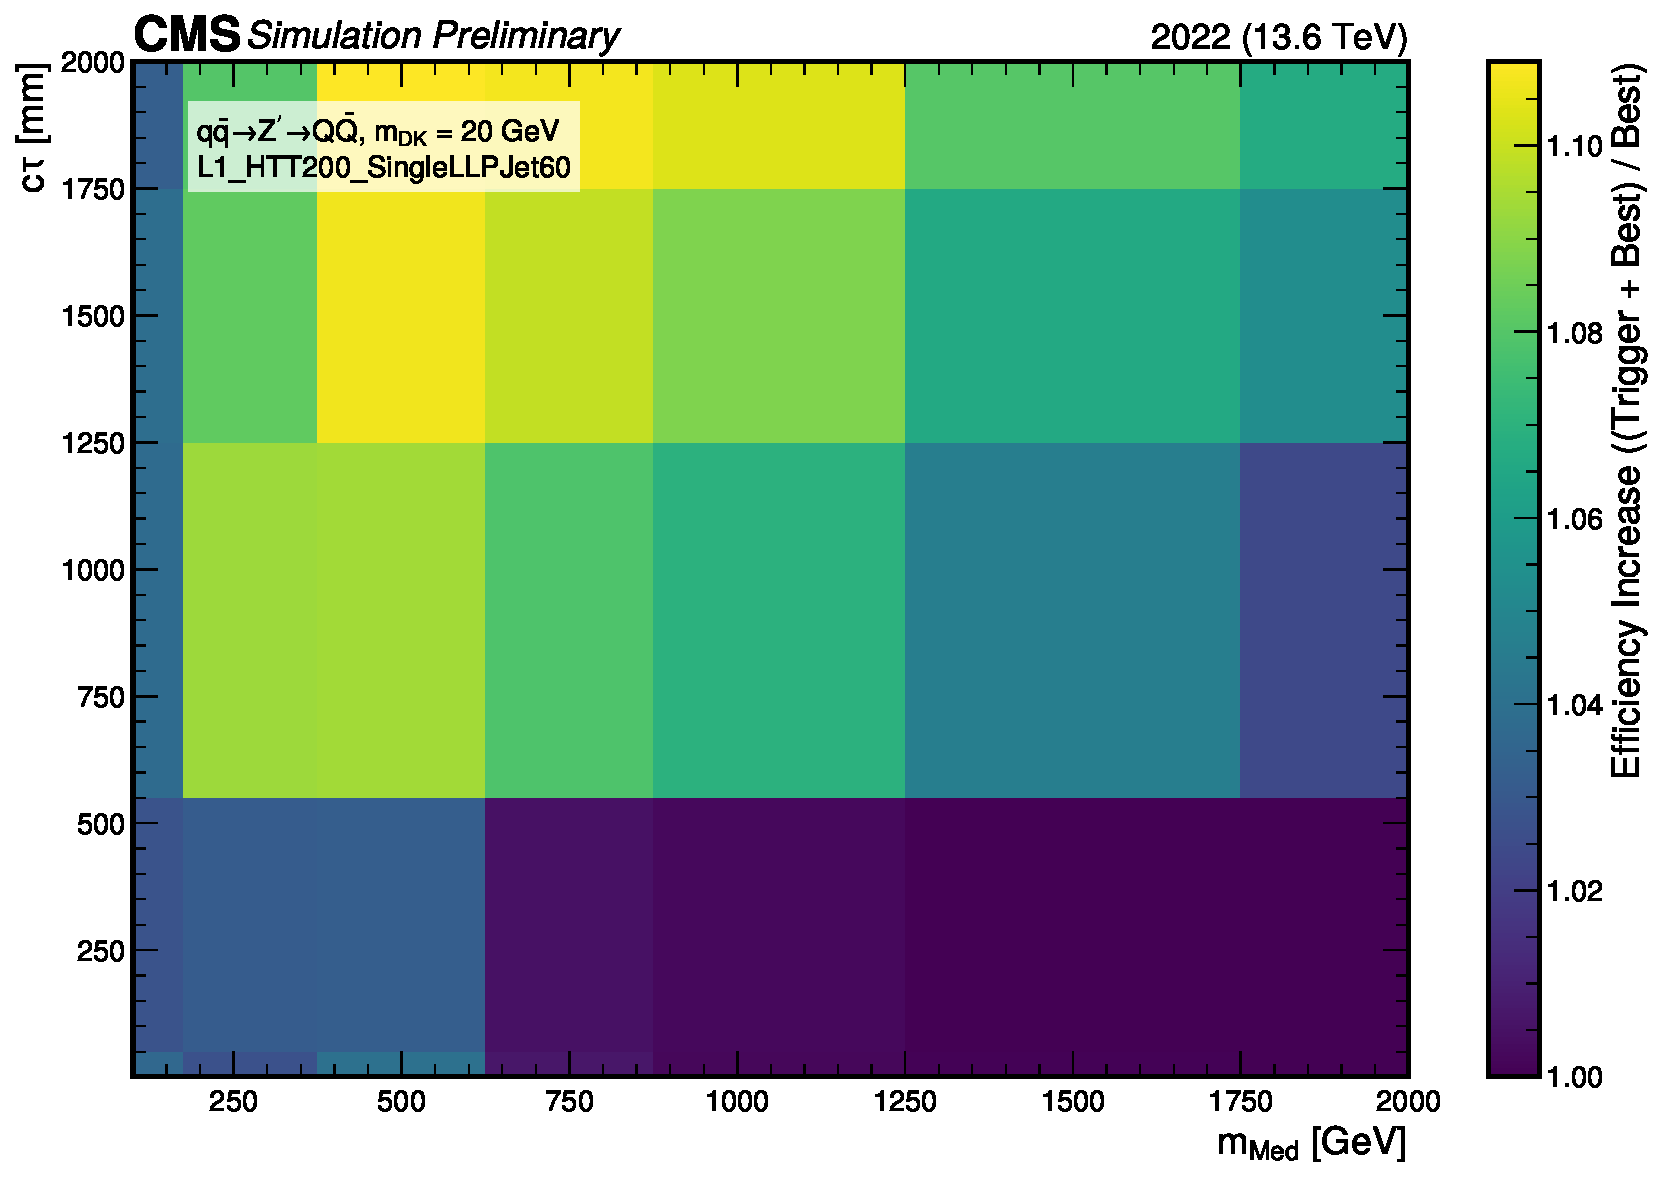
\includegraphics[width=\linewidth]{images/L1/llp_2D_schan/trigeffplots2D_L1_efftype-improv_s-channel_mDark-20_L1_HTT200_SingleLLPJet60_study_cloppear.pdf}
    \caption{Improvement, Z' mediator model}
    \label{fig:htt200singlellpjet60_improv_schan}
  \end{subfigure}

  \caption{Trigger efficiency heatmaps for \texttt{L1\_HTT200\_SingleLLPJet60} with $m_\mathrm{dark} = 20$ GeV in both the bifundamental and Z' mediator models. Each row shows a different efficiency definition: trigger-only, trigger+best object, and improvement.}
  \label{fig:htt200singlellpjet60_eff}
\end{figure}


\begin{figure}[h]
  \centering

  % Trigger-only
  \begin{subfigure}[t]{0.45\textwidth}
    \centering
    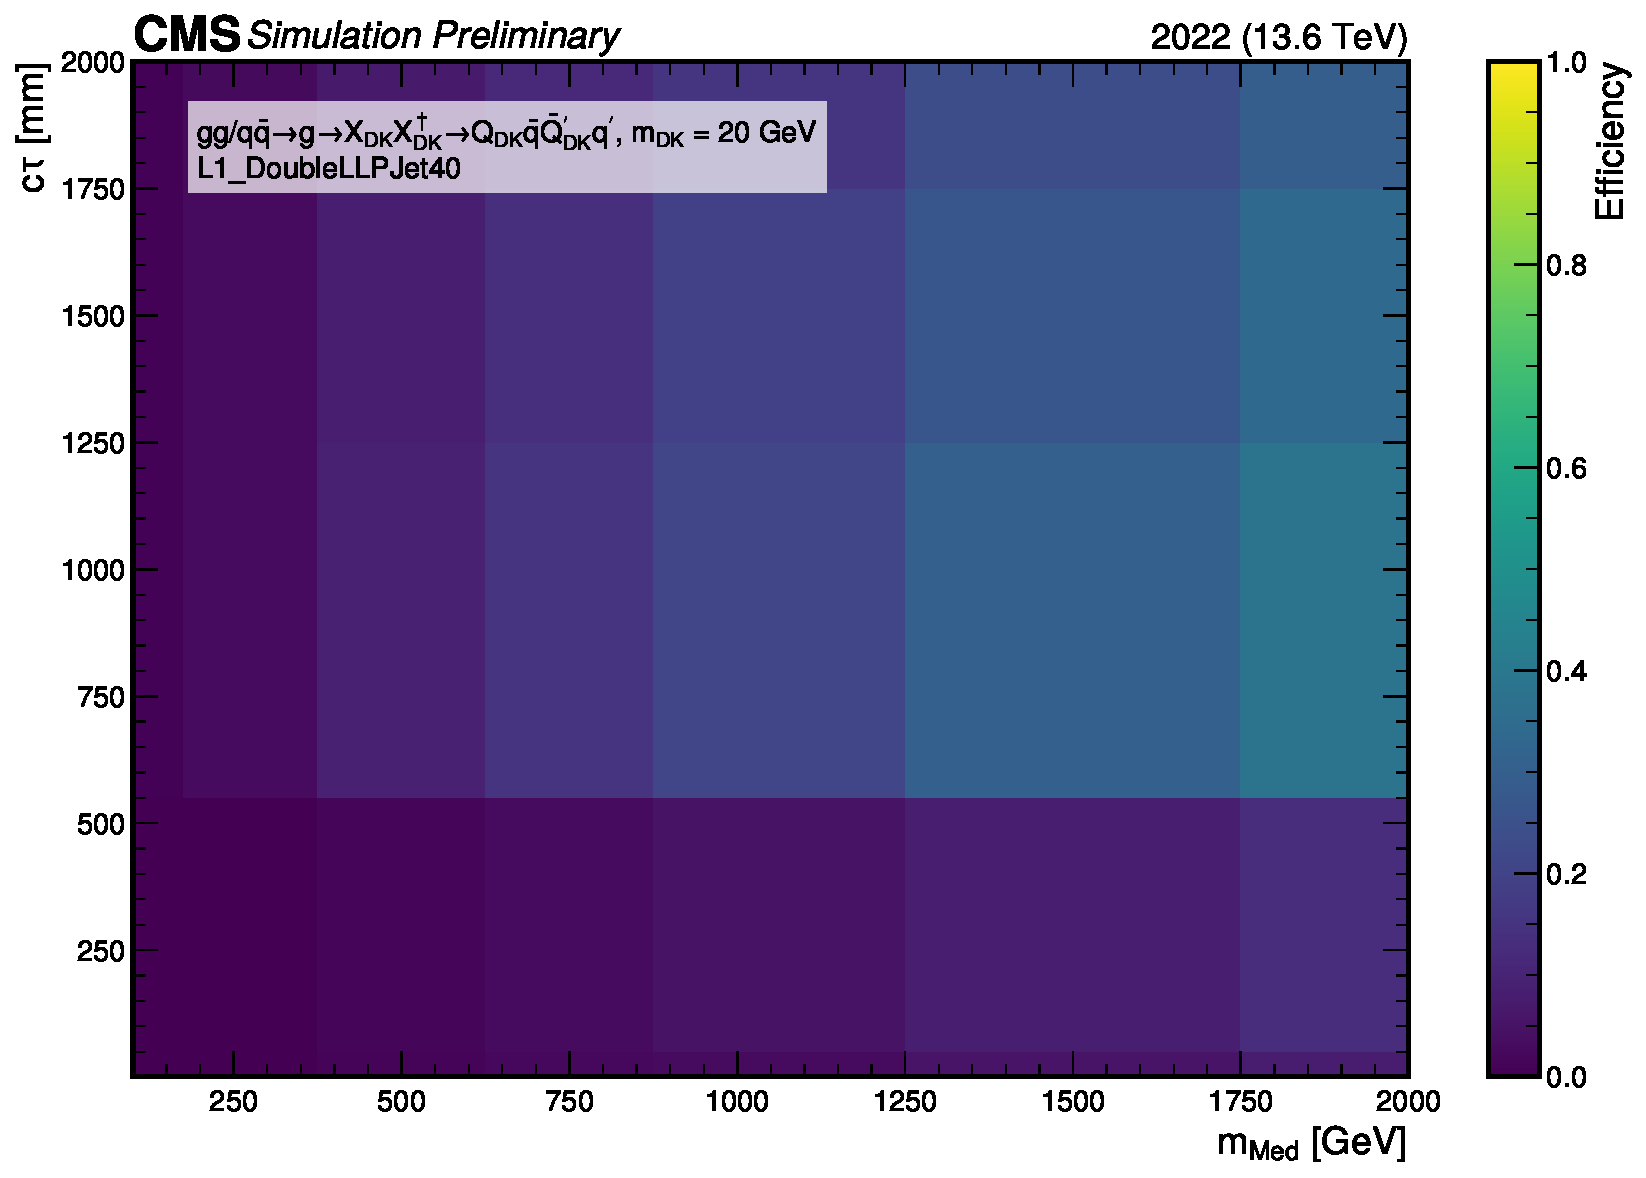
\includegraphics[width=\linewidth]{images/L1/llp_2D_tchan/trigeffplots2D_L1_efftype-trig_t-channel_mDark-20_L1_DoubleLLPJet40_study_cloppear.pdf}
    \caption{Trigger-only, Bifundamental mediator model}
    \label{fig:doublellp_trig_tchan}
  \end{subfigure}
  \hfill
  \begin{subfigure}[t]{0.45\textwidth}
    \centering
    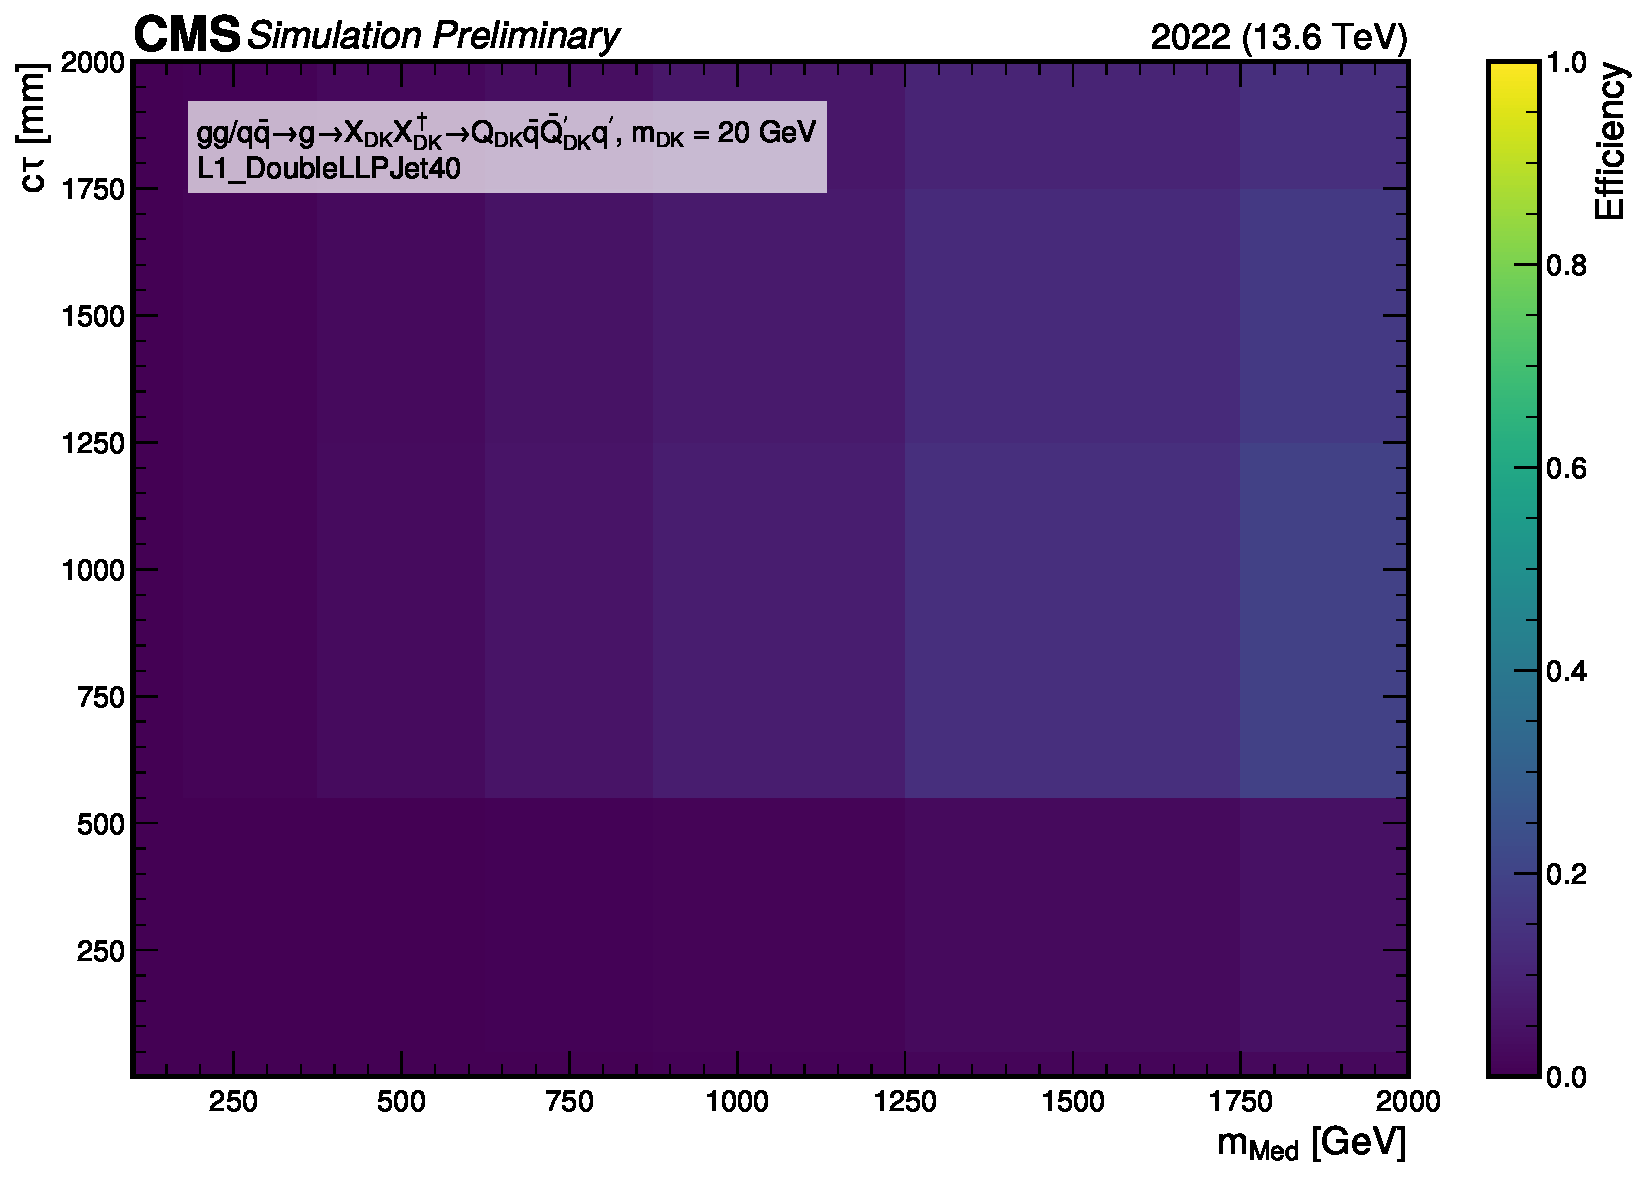
\includegraphics[width=\linewidth]{images/L1/llp_2D_schan/trigeffplots2D_L1_efftype-trig_s-channel_mDark-20_L1_DoubleLLPJet40_study_cloppear.pdf}
    \caption{Trigger-only, Z' mediator model}
    \label{fig:doublellp_trig_schan}
  \end{subfigure}

  \vspace{1em}

  % Trigger+best
  \begin{subfigure}[t]{0.45\textwidth}
    \centering
    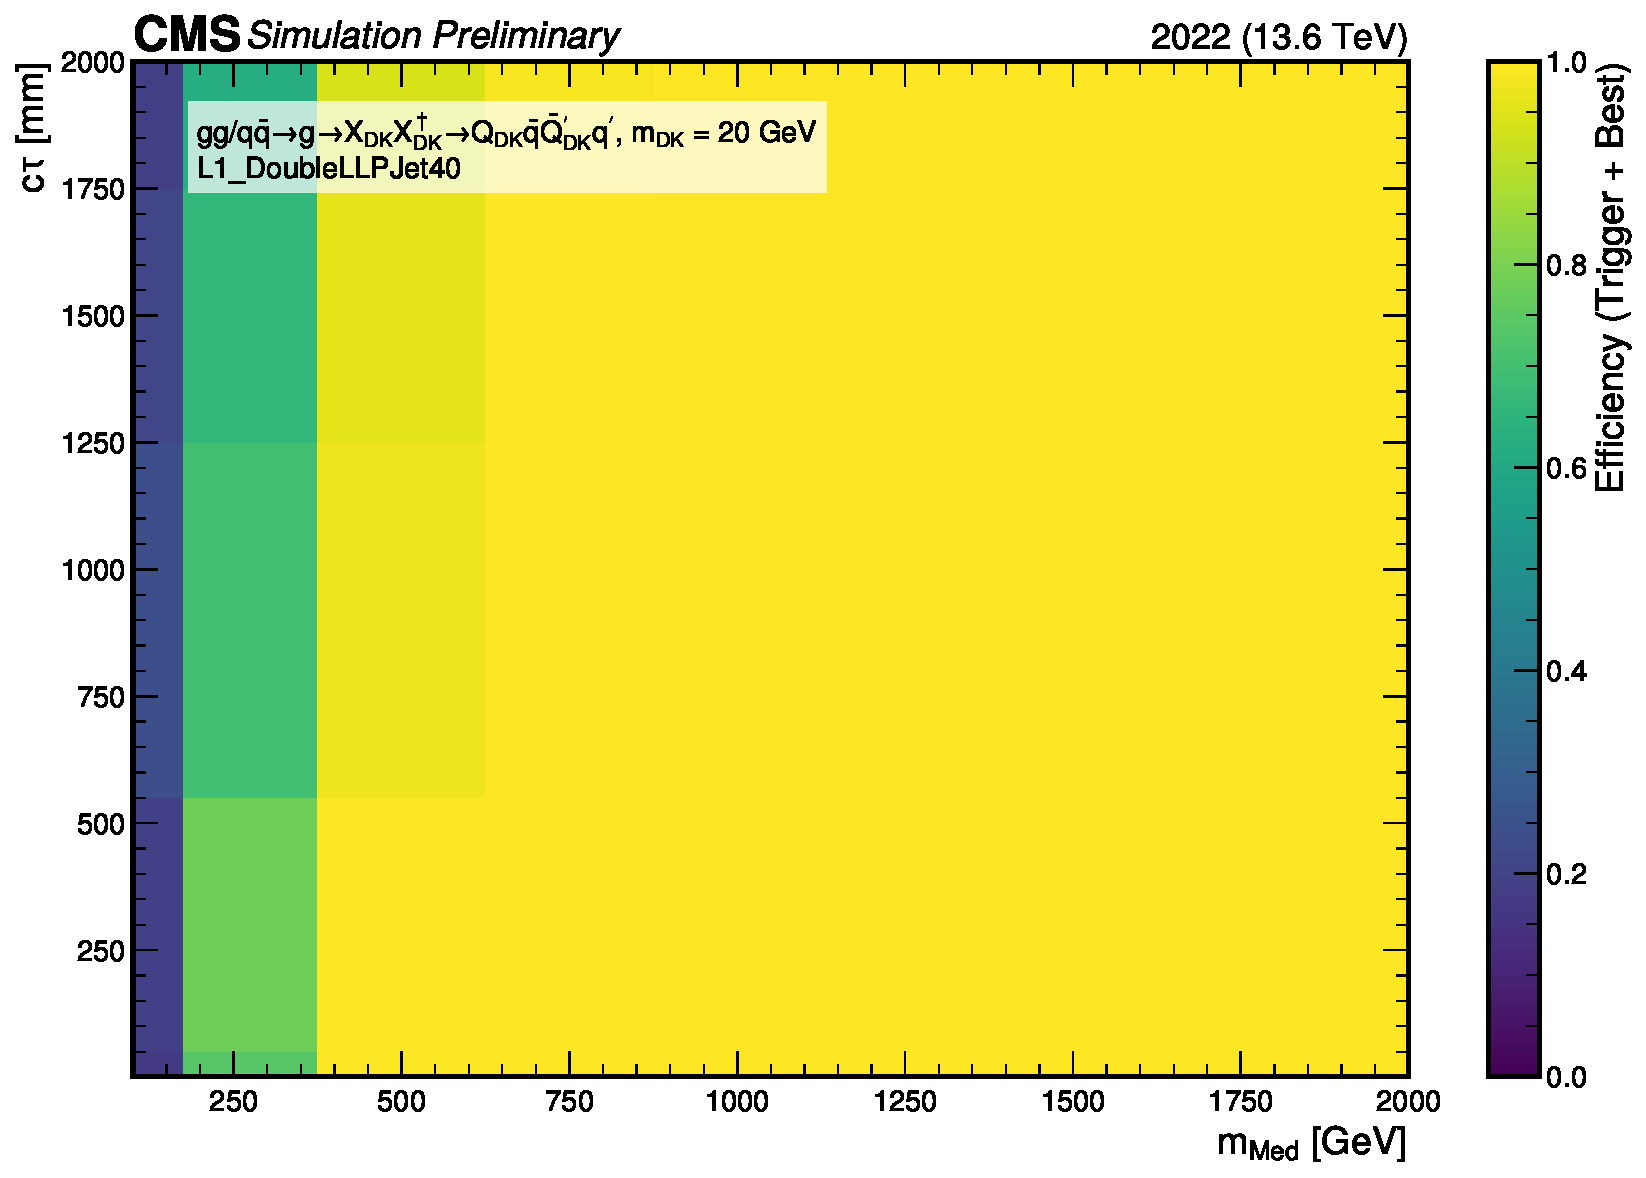
\includegraphics[width=\linewidth]{images/L1/llp_2D_tchan/trigeffplots2D_L1_efftype-trigplusbest_t-channel_mDark-20_L1_DoubleLLPJet40_study_cloppear.pdf}
    \caption{Trigger+best, Bifundamental mediator model}
    \label{fig:doublellp_trigplusbest_tchan}
  \end{subfigure}
  \hfill
  \begin{subfigure}[t]{0.45\textwidth}
    \centering
    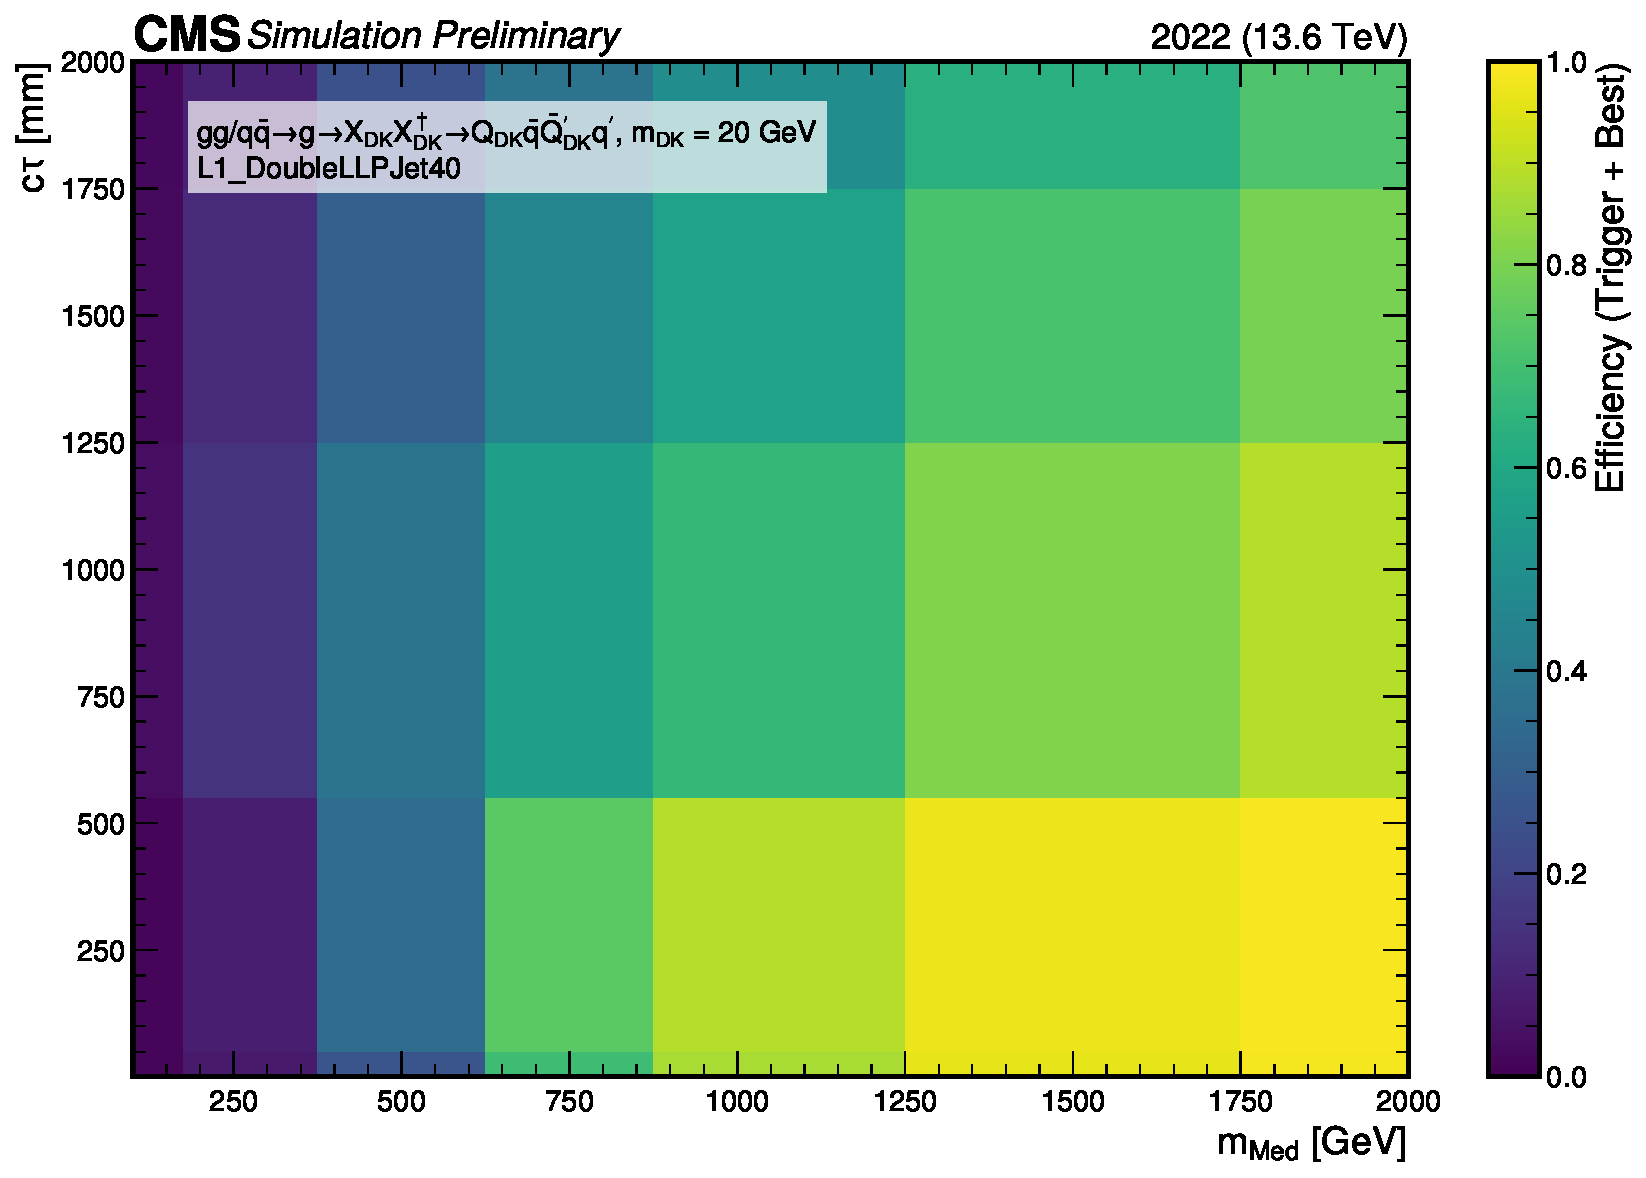
\includegraphics[width=\linewidth]{images/L1/llp_2D_schan/trigeffplots2D_L1_efftype-trigplusbest_s-channel_mDark-20_L1_DoubleLLPJet40_study_cloppear.pdf}
    \caption{Trigger+best, Z' mediator model}
    \label{fig:doublellp_trigplusbest_schan}
  \end{subfigure}

  \vspace{1em}

  % Improvement
  \begin{subfigure}[t]{0.45\textwidth}
    \centering
    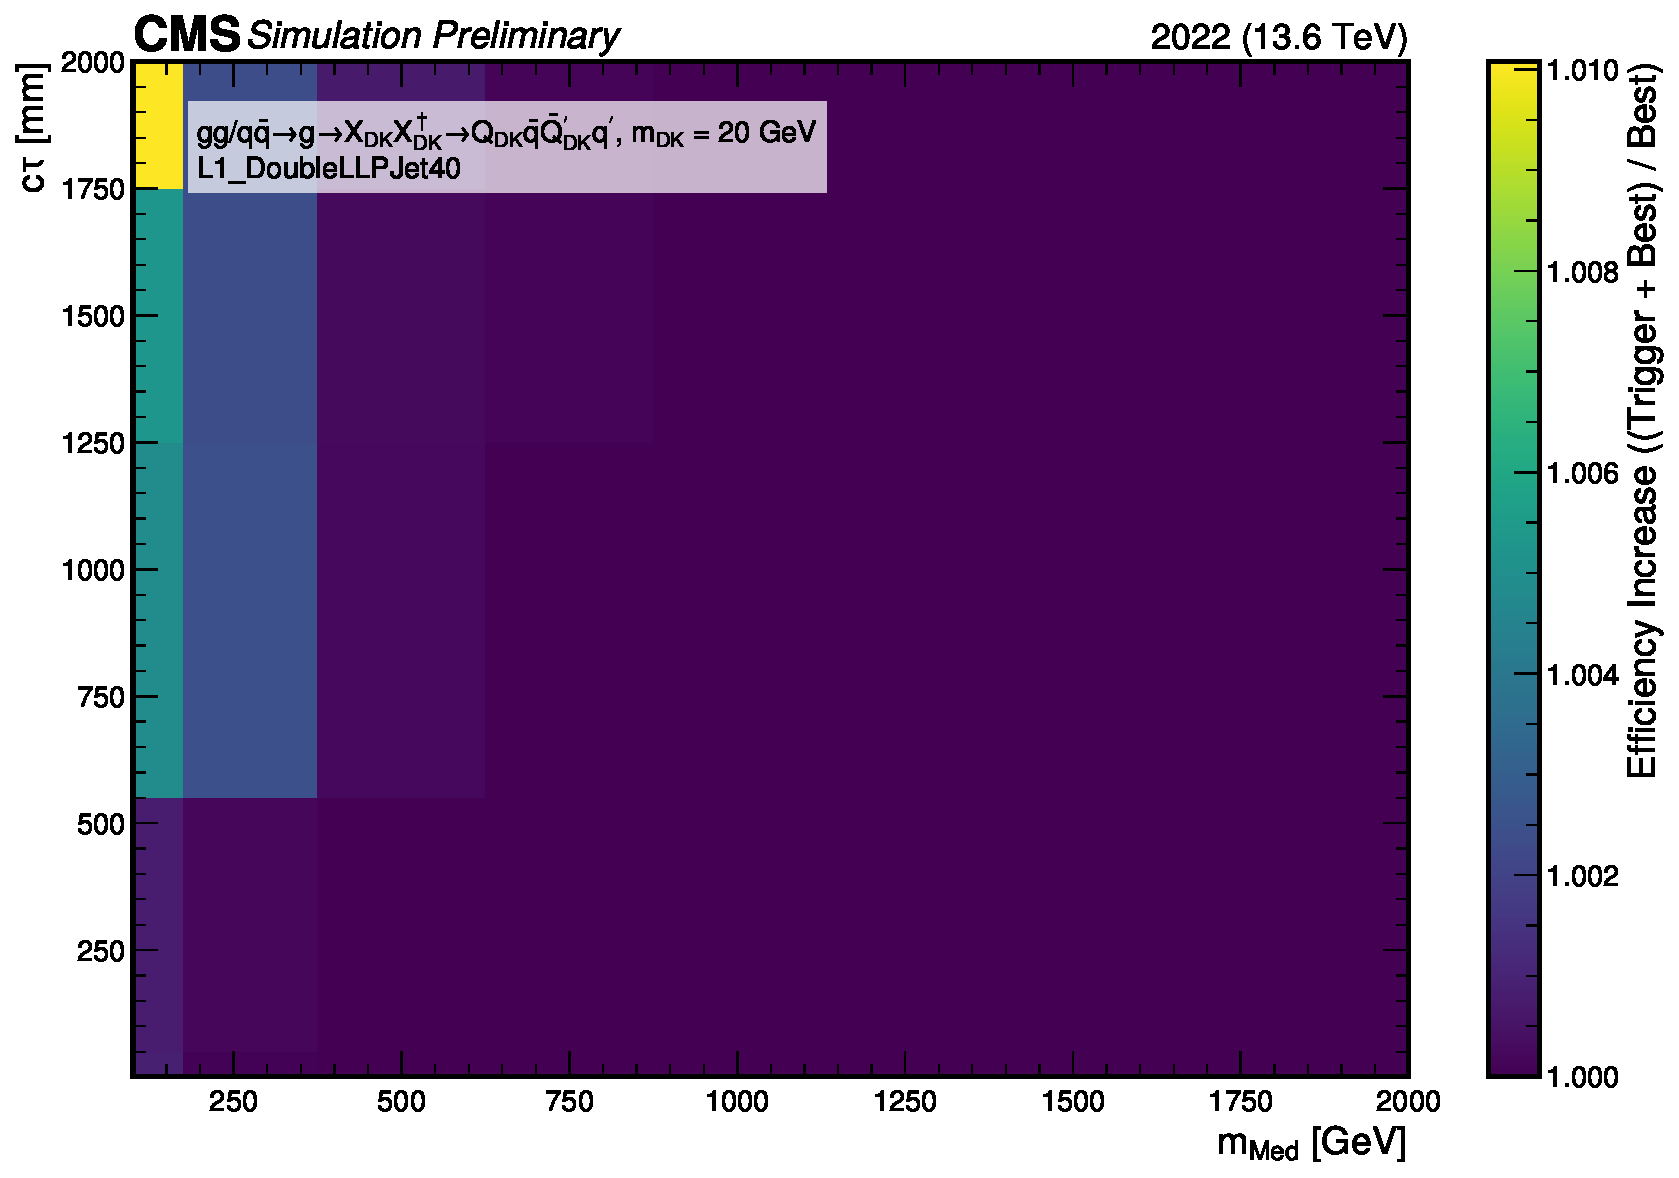
\includegraphics[width=\linewidth]{images/L1/llp_2D_tchan/trigeffplots2D_L1_efftype-improv_t-channel_mDark-20_L1_DoubleLLPJet40_study_cloppear.pdf}
    \caption{Improvement, Bifundamental mediator model}
    \label{fig:doublellp_improv_tchan}
  \end{subfigure}
  \hfill
  \begin{subfigure}[t]{0.45\textwidth}
    \centering
    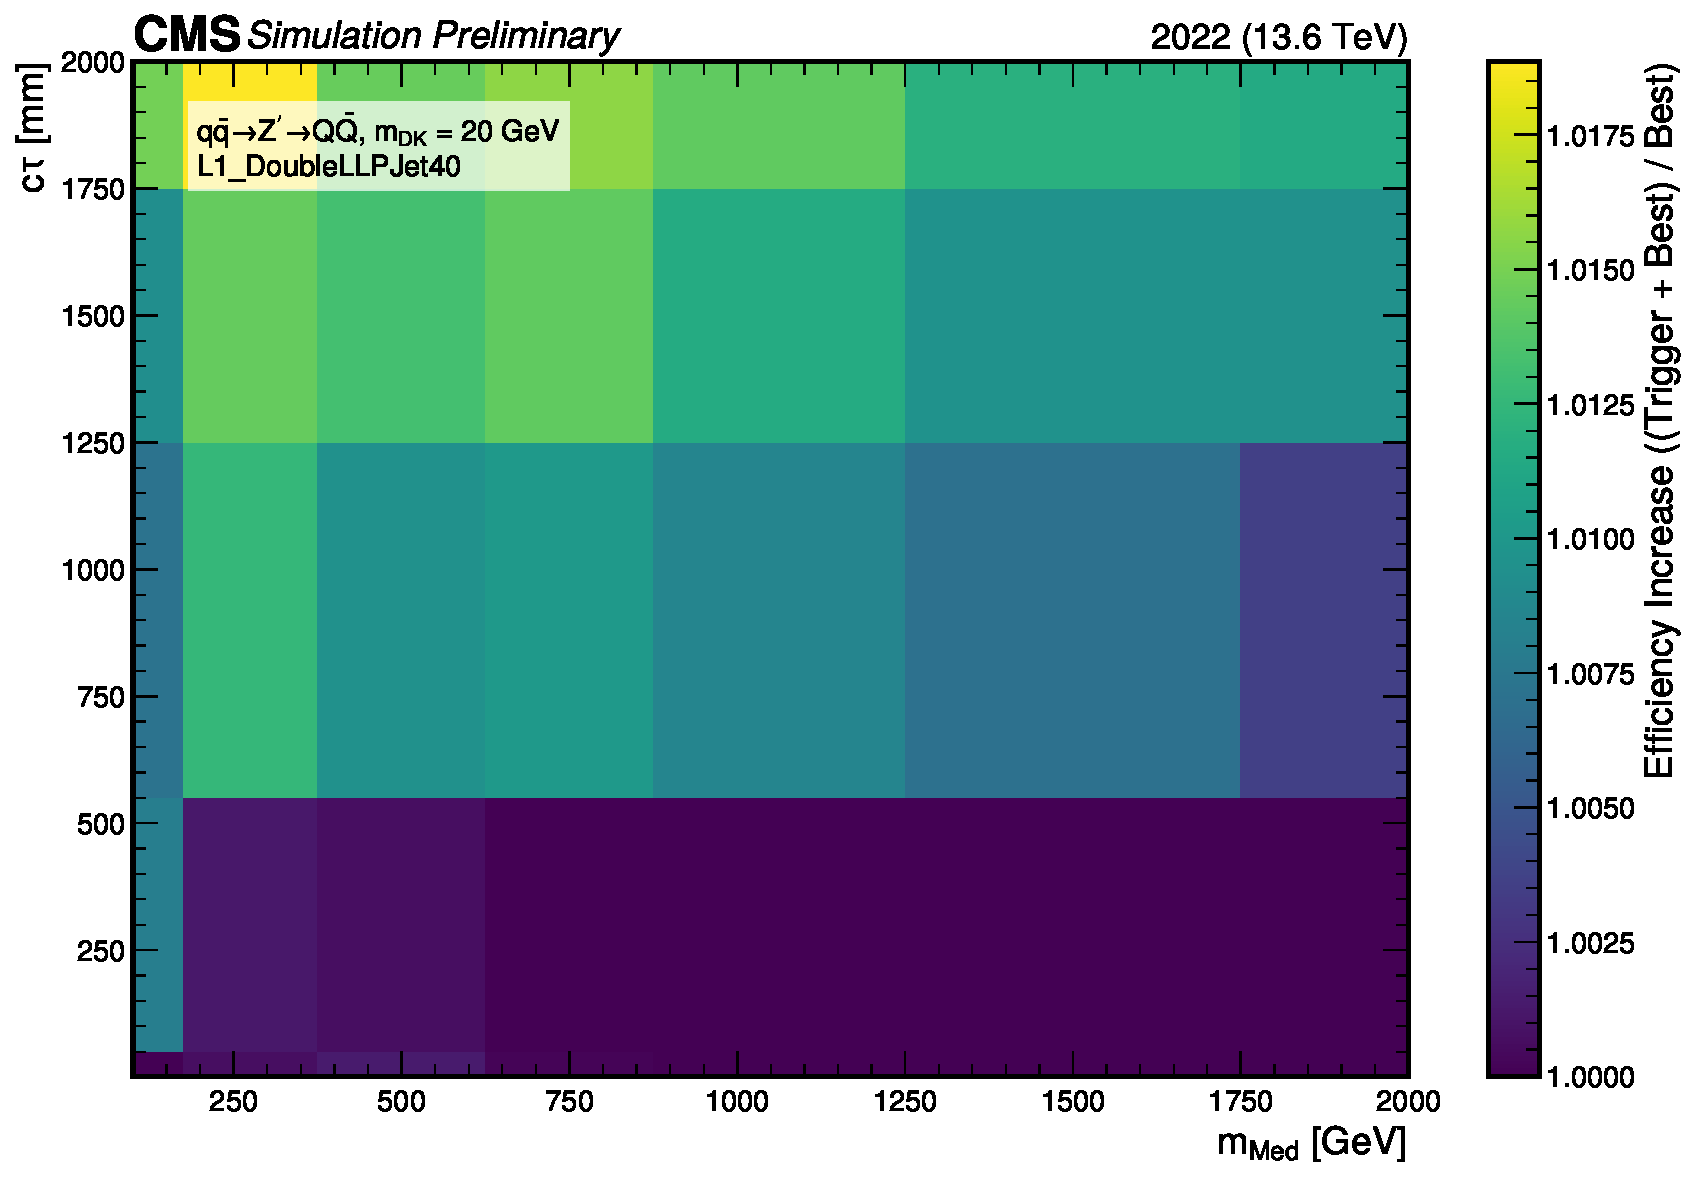
\includegraphics[width=\linewidth]{images/L1/llp_2D_schan/trigeffplots2D_L1_efftype-improv_s-channel_mDark-20_L1_DoubleLLPJet40_study_cloppear.pdf}
    \caption{Improvement, Z' mediator model}
    \label{fig:doublellp_improv_schan}
  \end{subfigure}

  \caption{Trigger efficiency heatmaps for \texttt{L1\_DoubleLLPJet40} with $m_\mathrm{dark} = 20$ GeV in both the bifundamental mediator model and the Z' mediator model. Each row shows a different efficiency definition: trigger-only, trigger+best object, and improvement.}
  \label{fig:doublellp_eff}
\end{figure}


The last L1 trigger that was studied was \texttt{L1\_SingleMuShower\_Nominal}. The raw efficiency map in Figures \ref{fig:mus_trig_tchan} and \ref{fig:mus_trig_schan} shows a similar behavior as was seen with the other LLP triggers: it targets models with higher $c\tau_{\text{dark}}$. In addition, it also has its peak $\text{EI}$ for higher dark pion lifetimes and lower mediator masses. However, a notable difference between this trigger and the previously discussed LLP triggers is that $\text{EI}$ is much higher. In Figure \ref{fig:mus_eff1D}, we can see that the increase in maximum $\text{EI}$ is nearly $1.6\times$ for the bifundamental model and approximately $4.5\times$ for $Z'$. These increases in efficiency are the highest that were observed for all of the L1 triggers under study.

% A notable result is that, when this trigger is used in conjuction with the best conventional triggers, unlike the other triggers studied, there is a notable impact on the efficiency map: for the Z' model, the efficiency of \texttt{L1\_SingleMuShower\_Nominal} with the best conventional triggers results in a notable increase in efficiency for models with lower $m_{\text{Med}}$ and higher $c\tau_{\text{dark}}$ when compared to just using the best triggers (Figure \ref{}).


\begin{figure}[h]
  \centering

  % Trigger-only
  \begin{subfigure}[t]{0.45\textwidth}
    \centering
    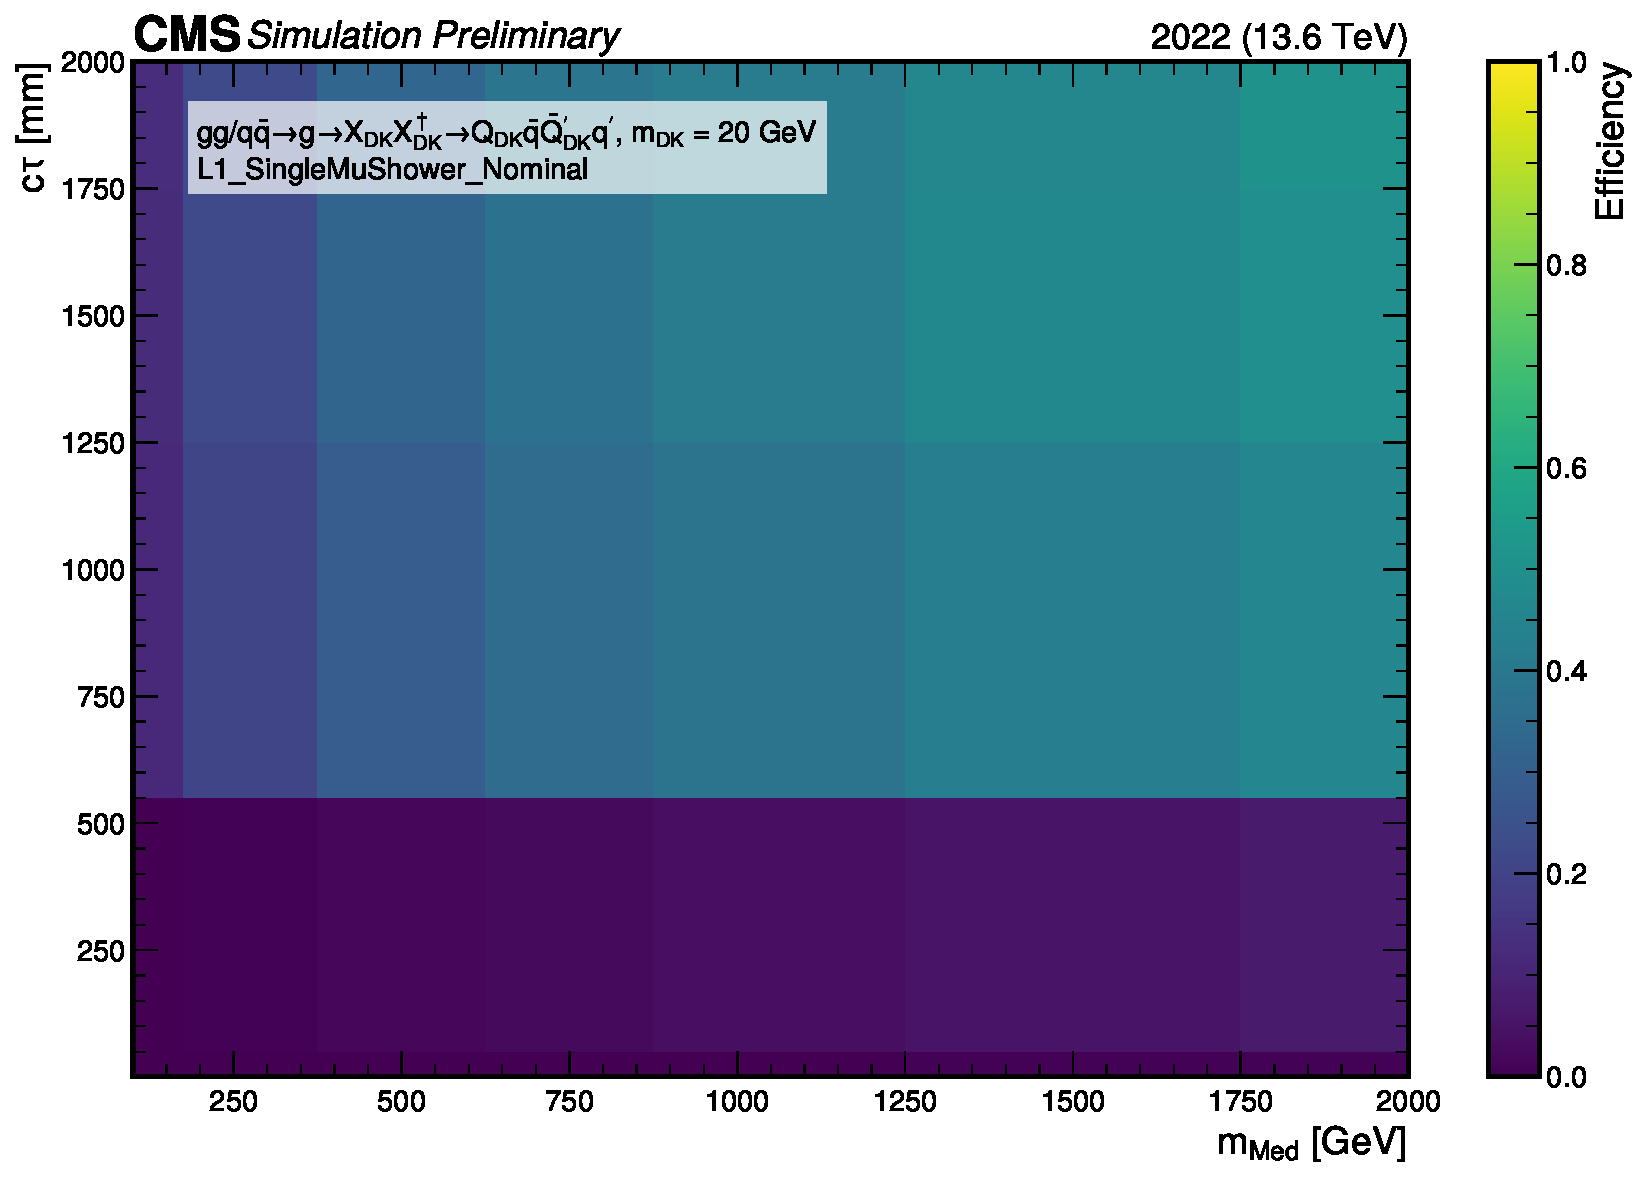
\includegraphics[width=\linewidth]{images/L1/llp_2D_tchan/trigeffplots2D_L1_efftype-trig_t-channel_mDark-20_L1_SingleMuShower_Nominal_study_cloppear.pdf}
    \caption{Trigger-only, Bifundamental mediator model}
    \label{fig:mus_trig_tchan}
  \end{subfigure}
  \hfill
  \begin{subfigure}[t]{0.45\textwidth}
    \centering
    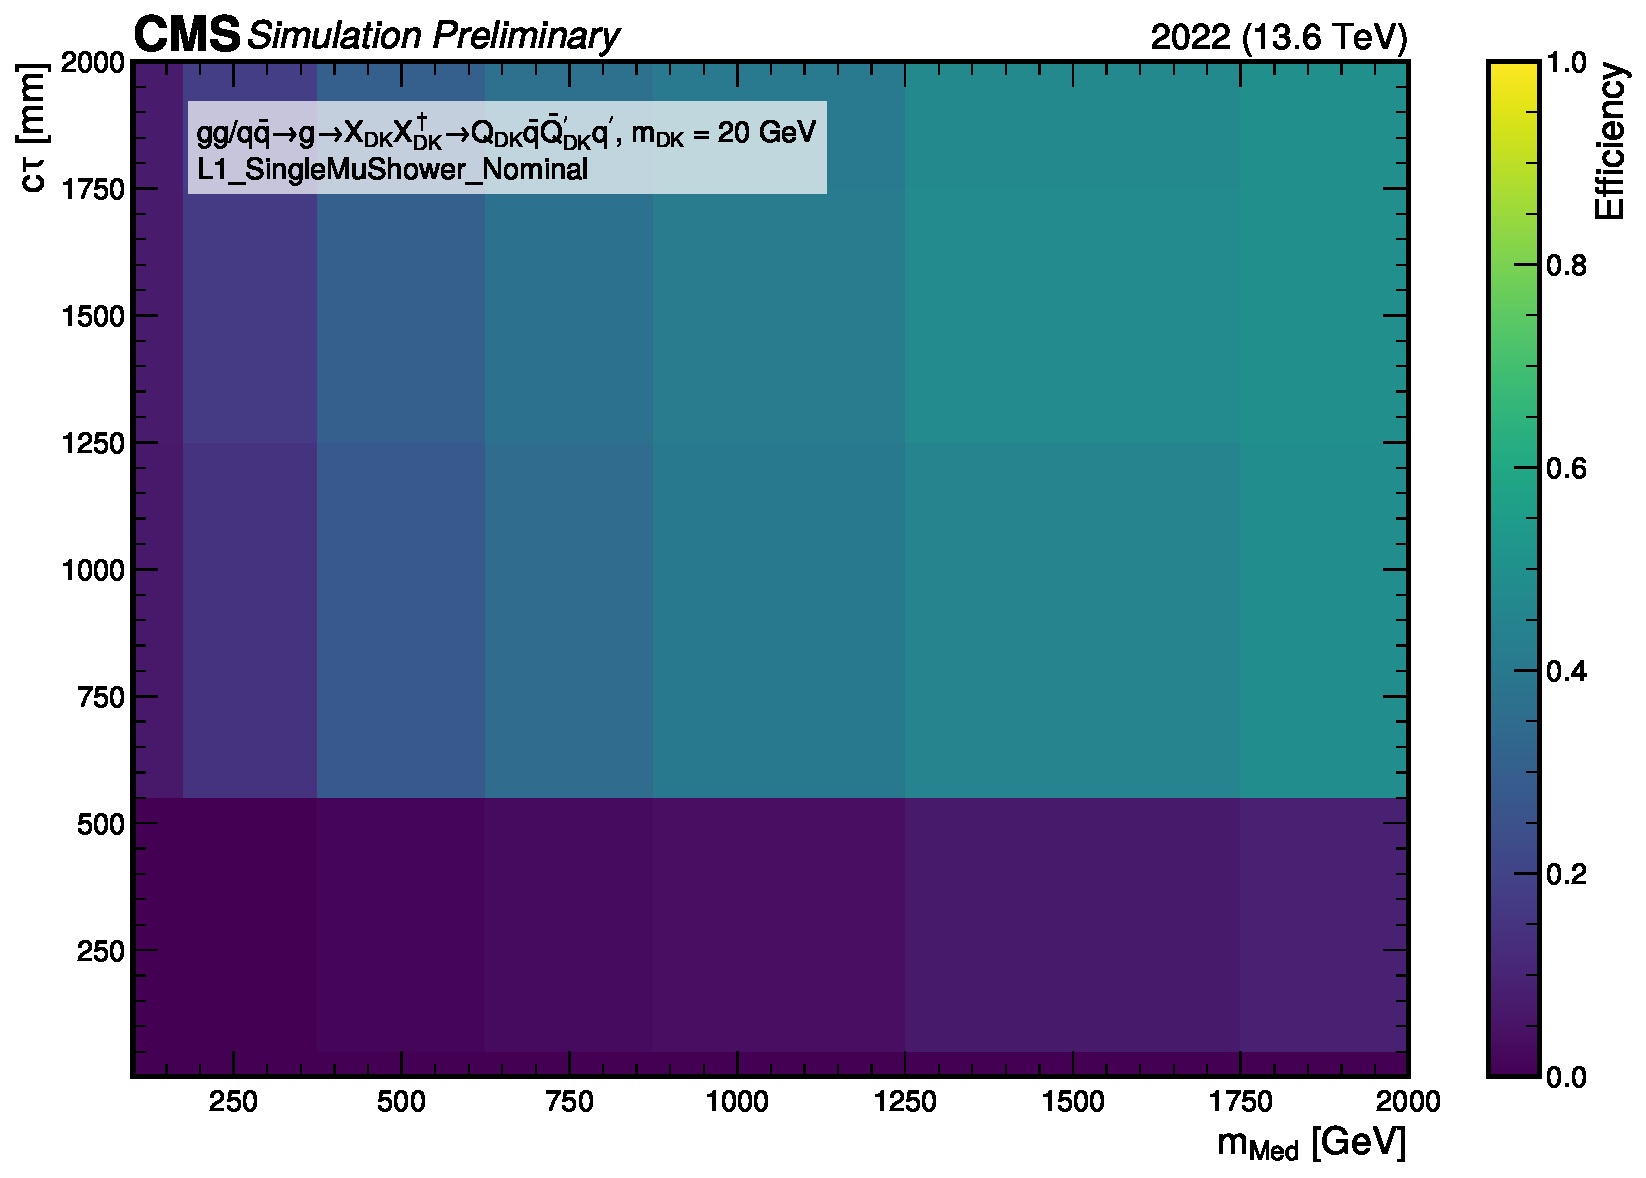
\includegraphics[width=\linewidth]{images/L1/llp_2D_schan/trigeffplots2D_L1_efftype-trig_s-channel_mDark-20_L1_SingleMuShower_Nominal_study_cloppear.pdf}
    \caption{Trigger-only, Z' mediator model}
    \label{fig:mus_trig_schan}
  \end{subfigure}

  \vspace{1em}

  % Trigger+best
  \begin{subfigure}[t]{0.45\textwidth}
    \centering
    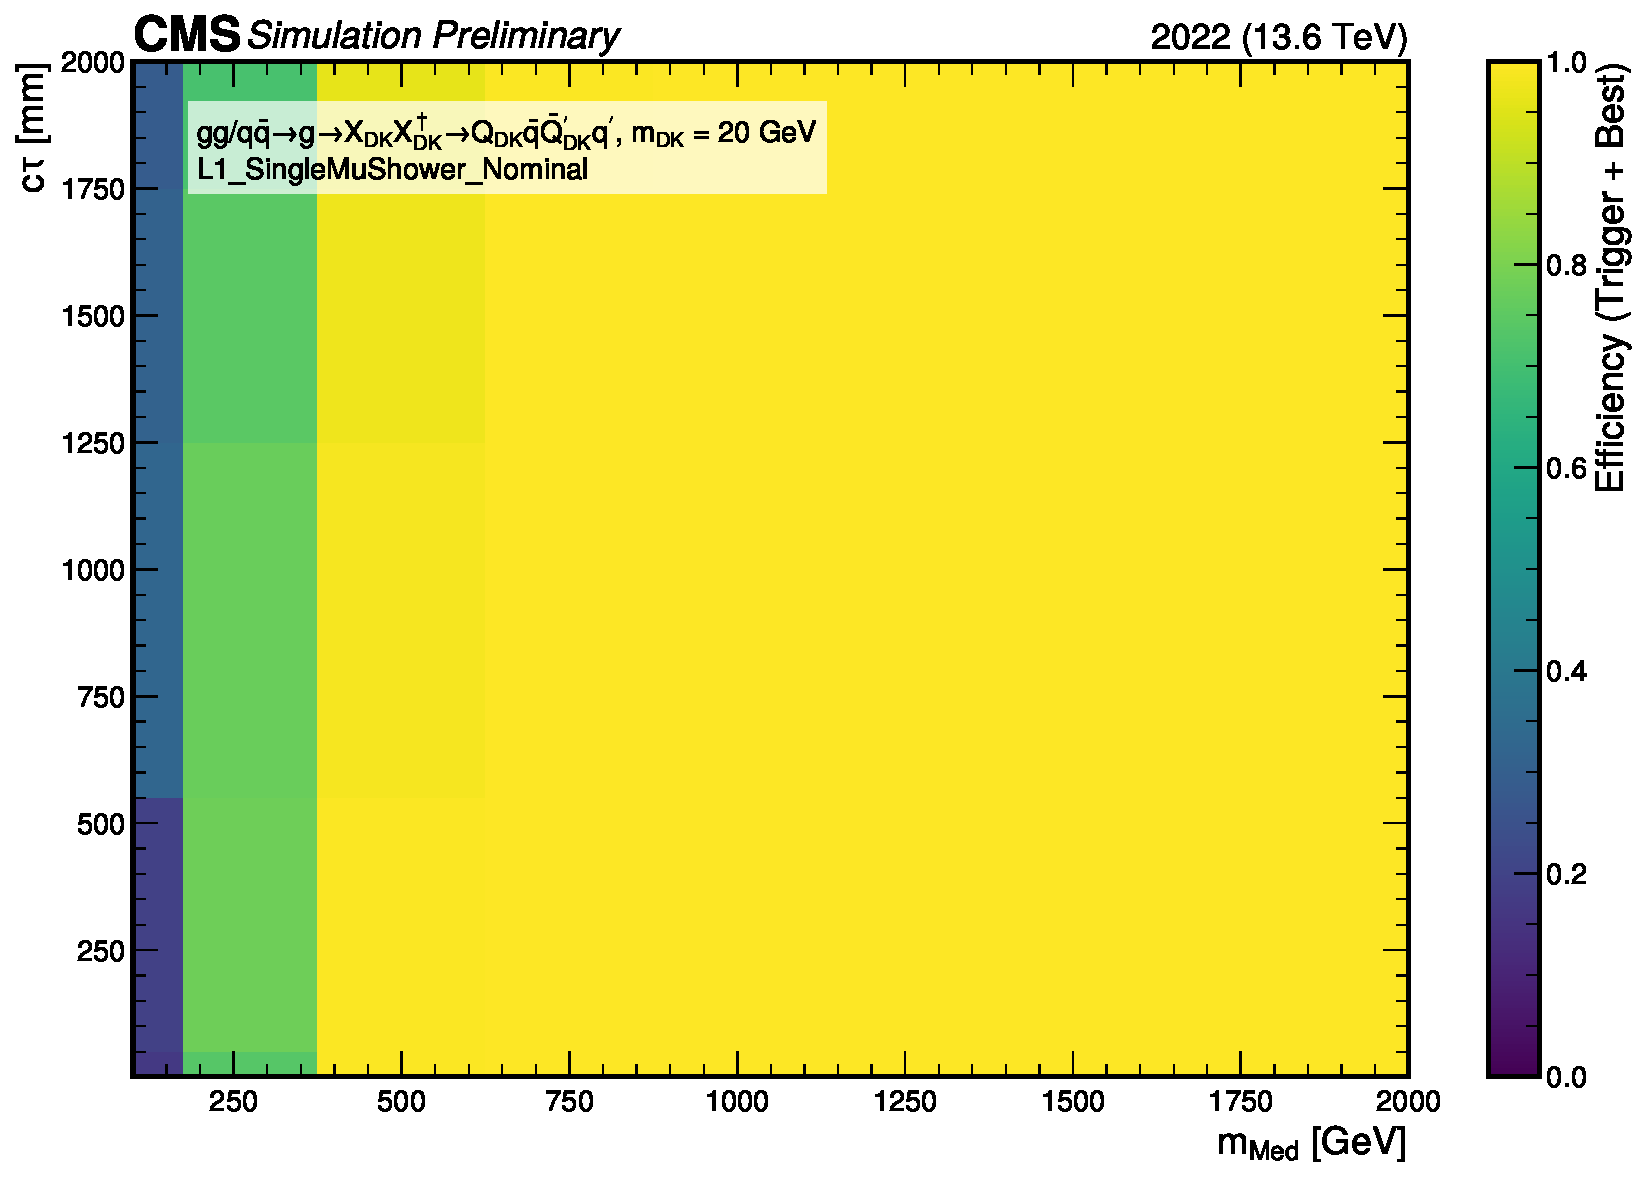
\includegraphics[width=\linewidth]{images/L1/llp_2D_tchan/trigeffplots2D_L1_efftype-trigplusbest_t-channel_mDark-20_L1_SingleMuShower_Nominal_study_cloppear.pdf}
    \caption{Trigger+best, Bifundamental mediator model}
    \label{fig:mus_trigplusbest_tchan}
  \end{subfigure}
  \hfill
  \begin{subfigure}[t]{0.45\textwidth}
    \centering
    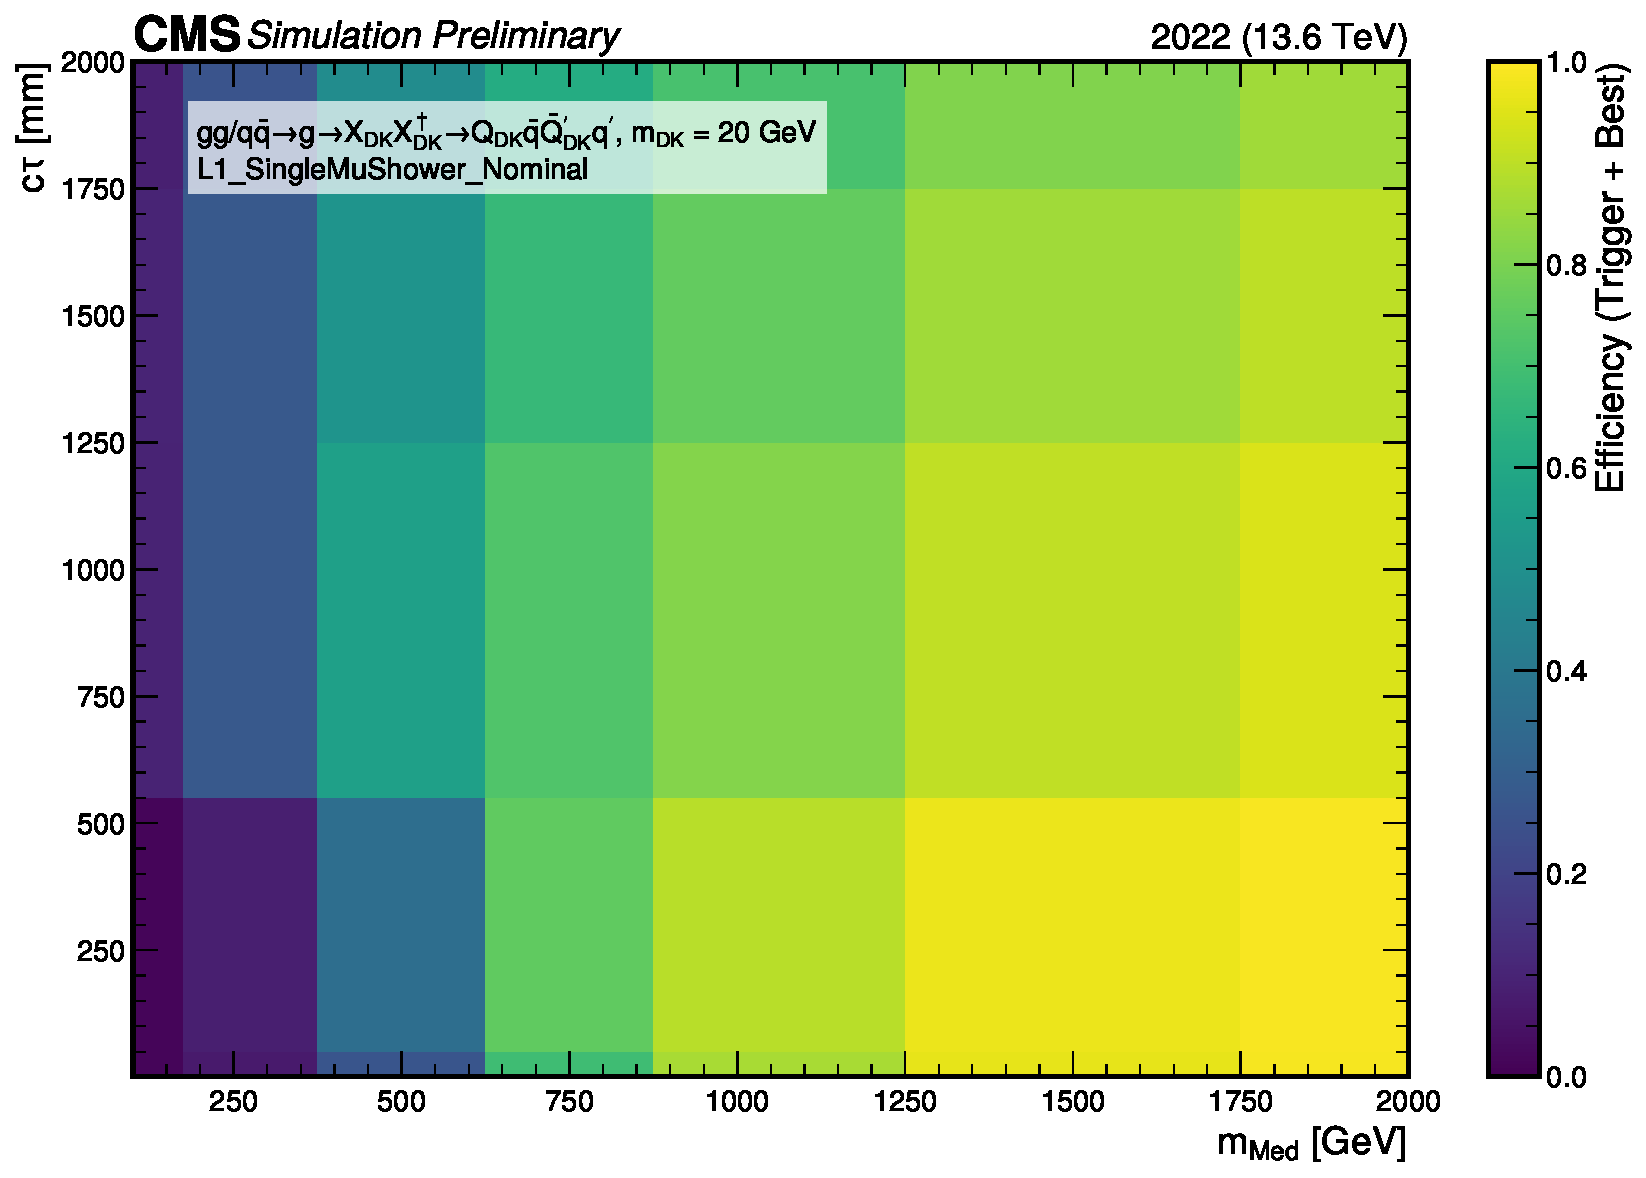
\includegraphics[width=\linewidth]{images/L1/llp_2D_schan/trigeffplots2D_L1_efftype-trigplusbest_s-channel_mDark-20_L1_SingleMuShower_Nominal_study_cloppear.pdf}
    \caption{Trigger+best, Z' mediator model}
    \label{fig:mus_trigplusbest_schan}
  \end{subfigure}

  \vspace{1em}

  % Improvement
  \begin{subfigure}[t]{0.45\textwidth}
    \centering
    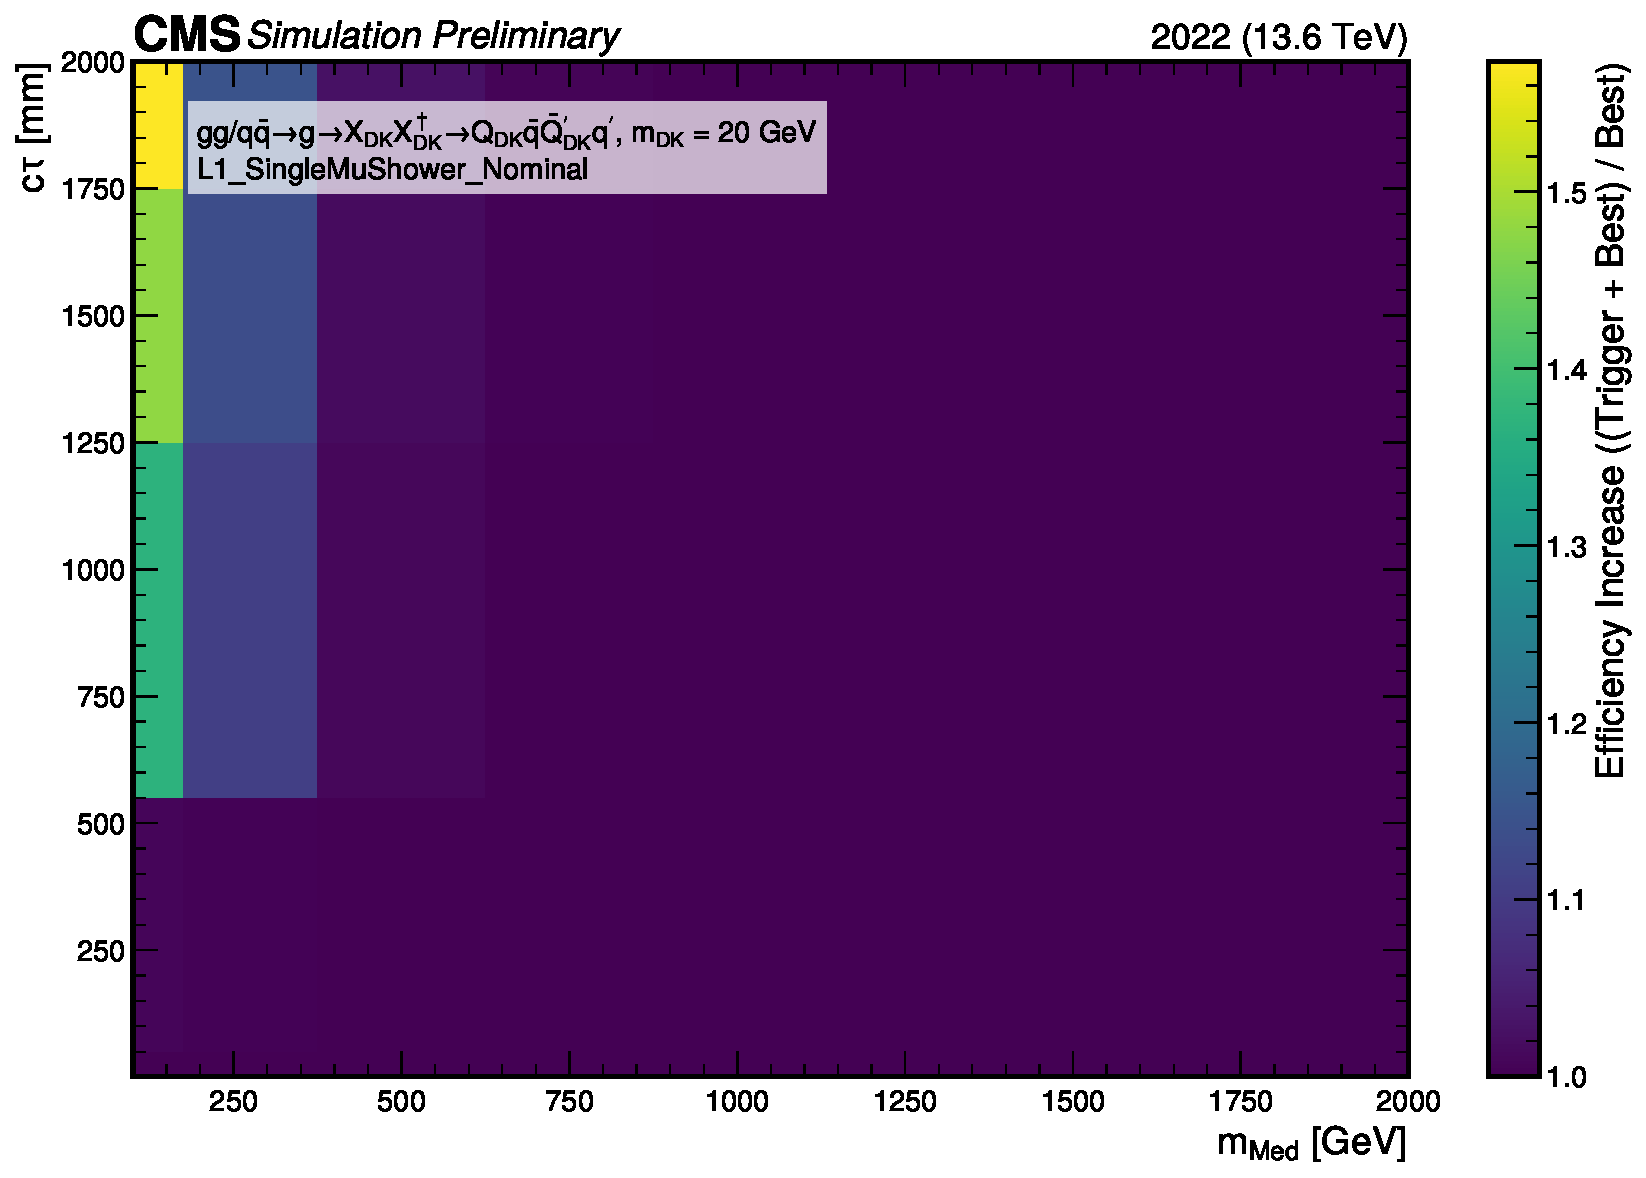
\includegraphics[width=\linewidth]{images/L1/llp_2D_tchan/trigeffplots2D_L1_efftype-improv_t-channel_mDark-20_L1_SingleMuShower_Nominal_study_cloppear.pdf}
    \caption{Improvement, Bifundamental mediator model}
    \label{fig:mus_improv_tchan}
  \end{subfigure}
  \hfill
  \begin{subfigure}[t]{0.45\textwidth}
    \centering
    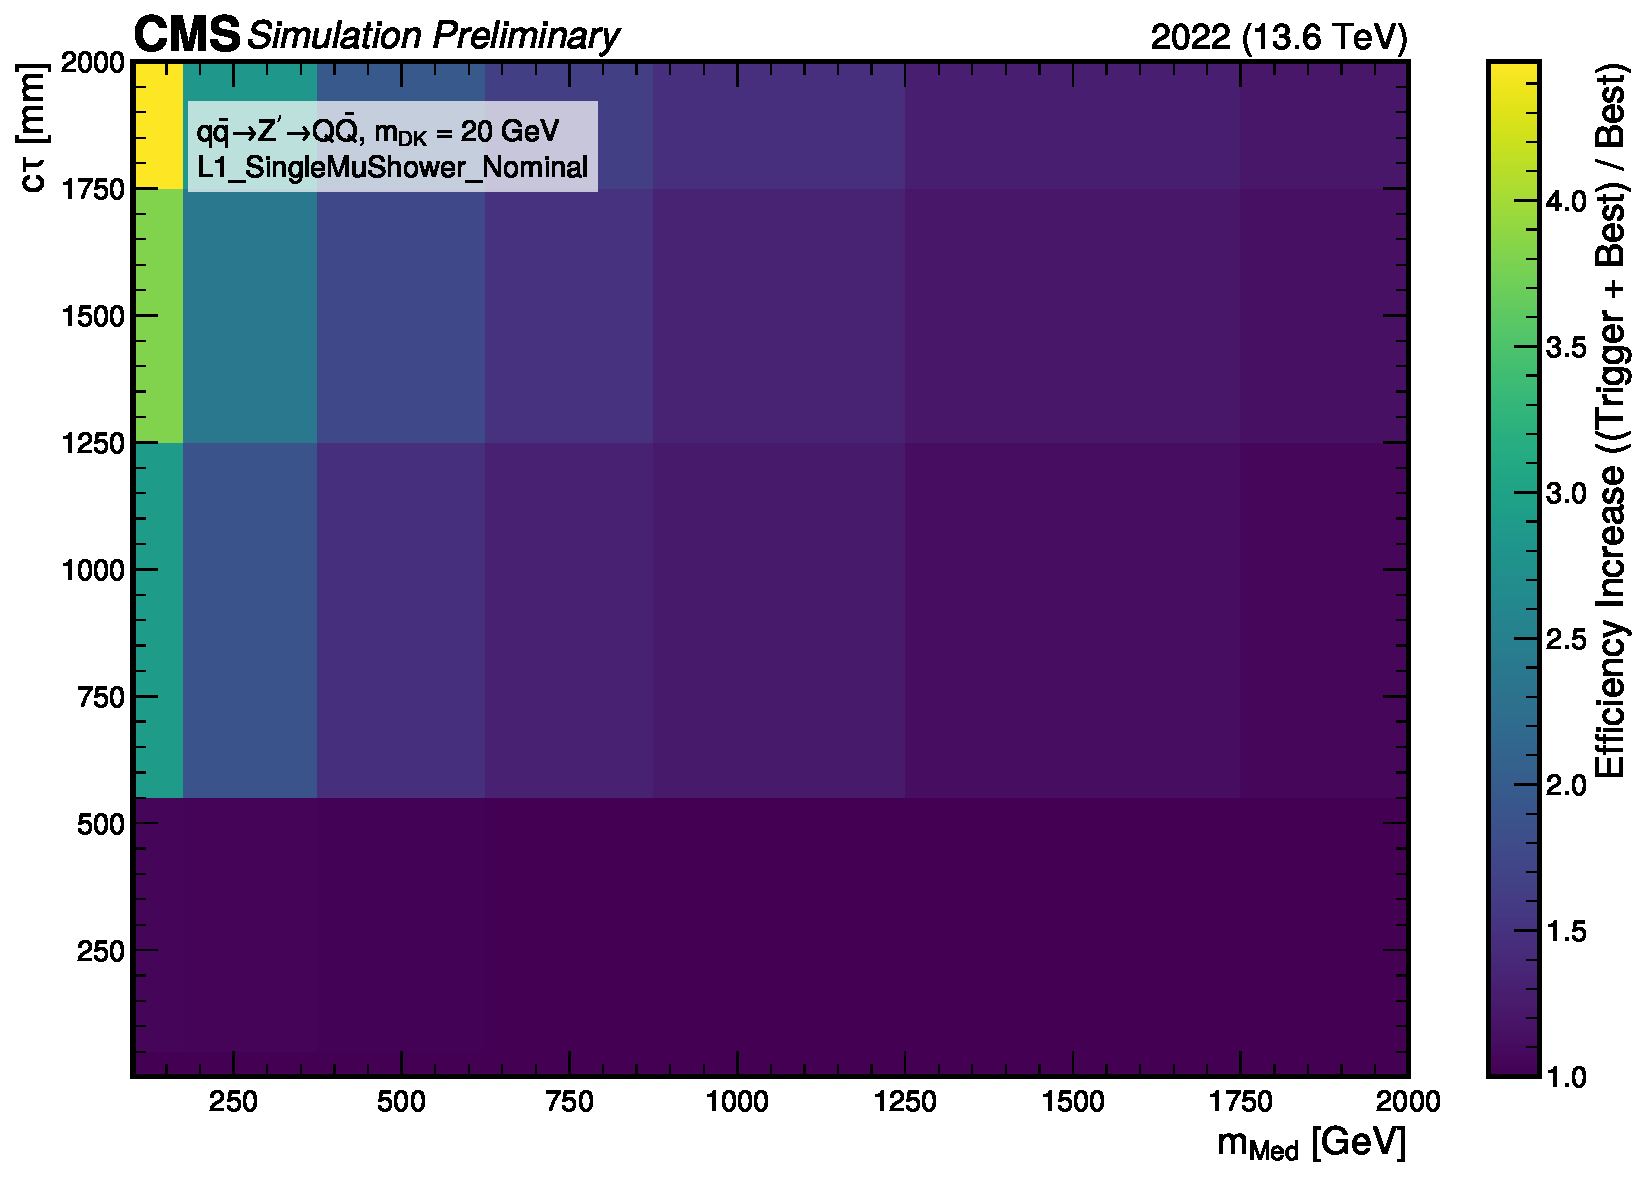
\includegraphics[width=\linewidth]{images/L1/llp_2D_schan/trigeffplots2D_L1_efftype-improv_s-channel_mDark-20_L1_SingleMuShower_Nominal_study_cloppear.pdf}
    \caption{Improvement, Z' mediator model}
    \label{fig:mus_improv_schan}
  \end{subfigure}

  \caption{Trigger efficiency heatmaps for \texttt{L1\_SingleMuShower\_Nominal} with $m_\mathrm{dark} = 20$ GeV in both the bifundamental mediator model and the Z' mediator model. Each row shows a different efficiency definition: trigger-only, trigger+best object, and improvement.}
  \label{fig:mus_eff}
\end{figure}

\begin{figure}[h]
  \centering

  % Bifundamental mediator model (t-channel)
  \begin{subfigure}[t]{0.45\textwidth}
    \centering
    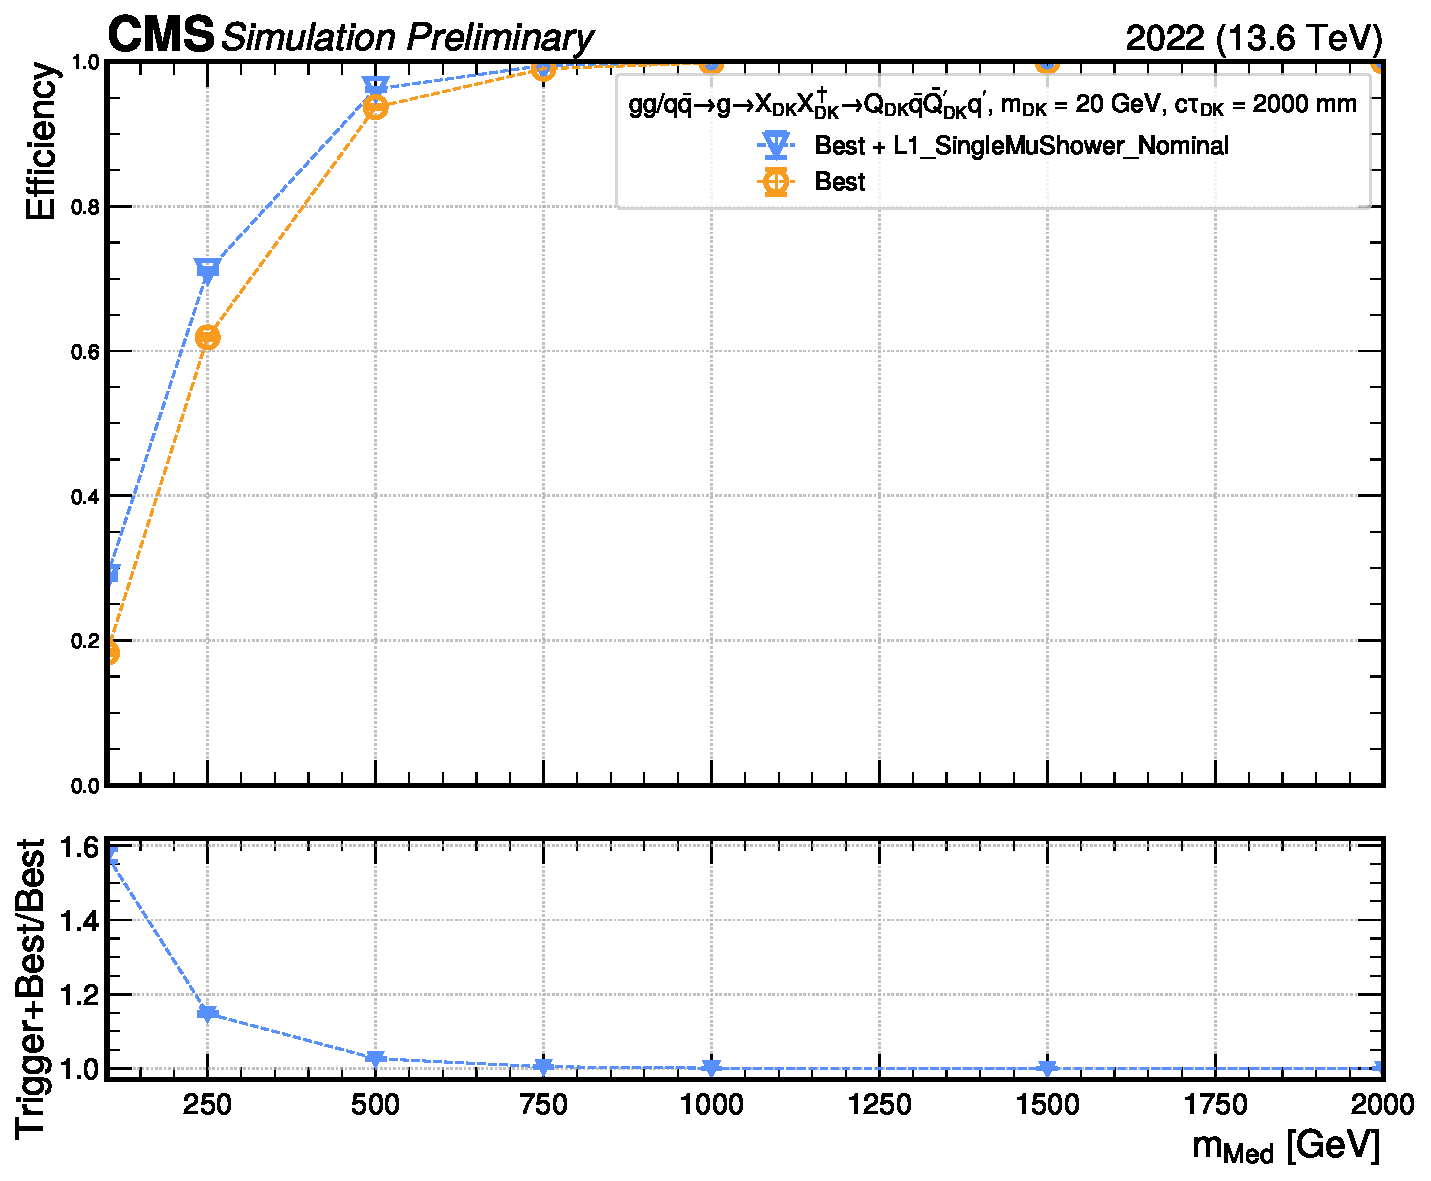
\includegraphics[width=\linewidth]{images/L1/llp_1D_tchan/trigeffplots1D_L1_efftype-trigplusbest_t-channel_mDark-20_ctau-2000_L1_SingleMuShower_Nominal_study_cloppear.pdf}
    \caption{Trigger+best efficiency for $c\tau = 2000$ mm, Bifundamental mediator model}
    \label{fig:mus_eff1D_ctau2000_tchan}
  \end{subfigure}
  \hfill
  % Z' mediator model (s-channel)
  \begin{subfigure}[t]{0.45\textwidth}
    \centering
    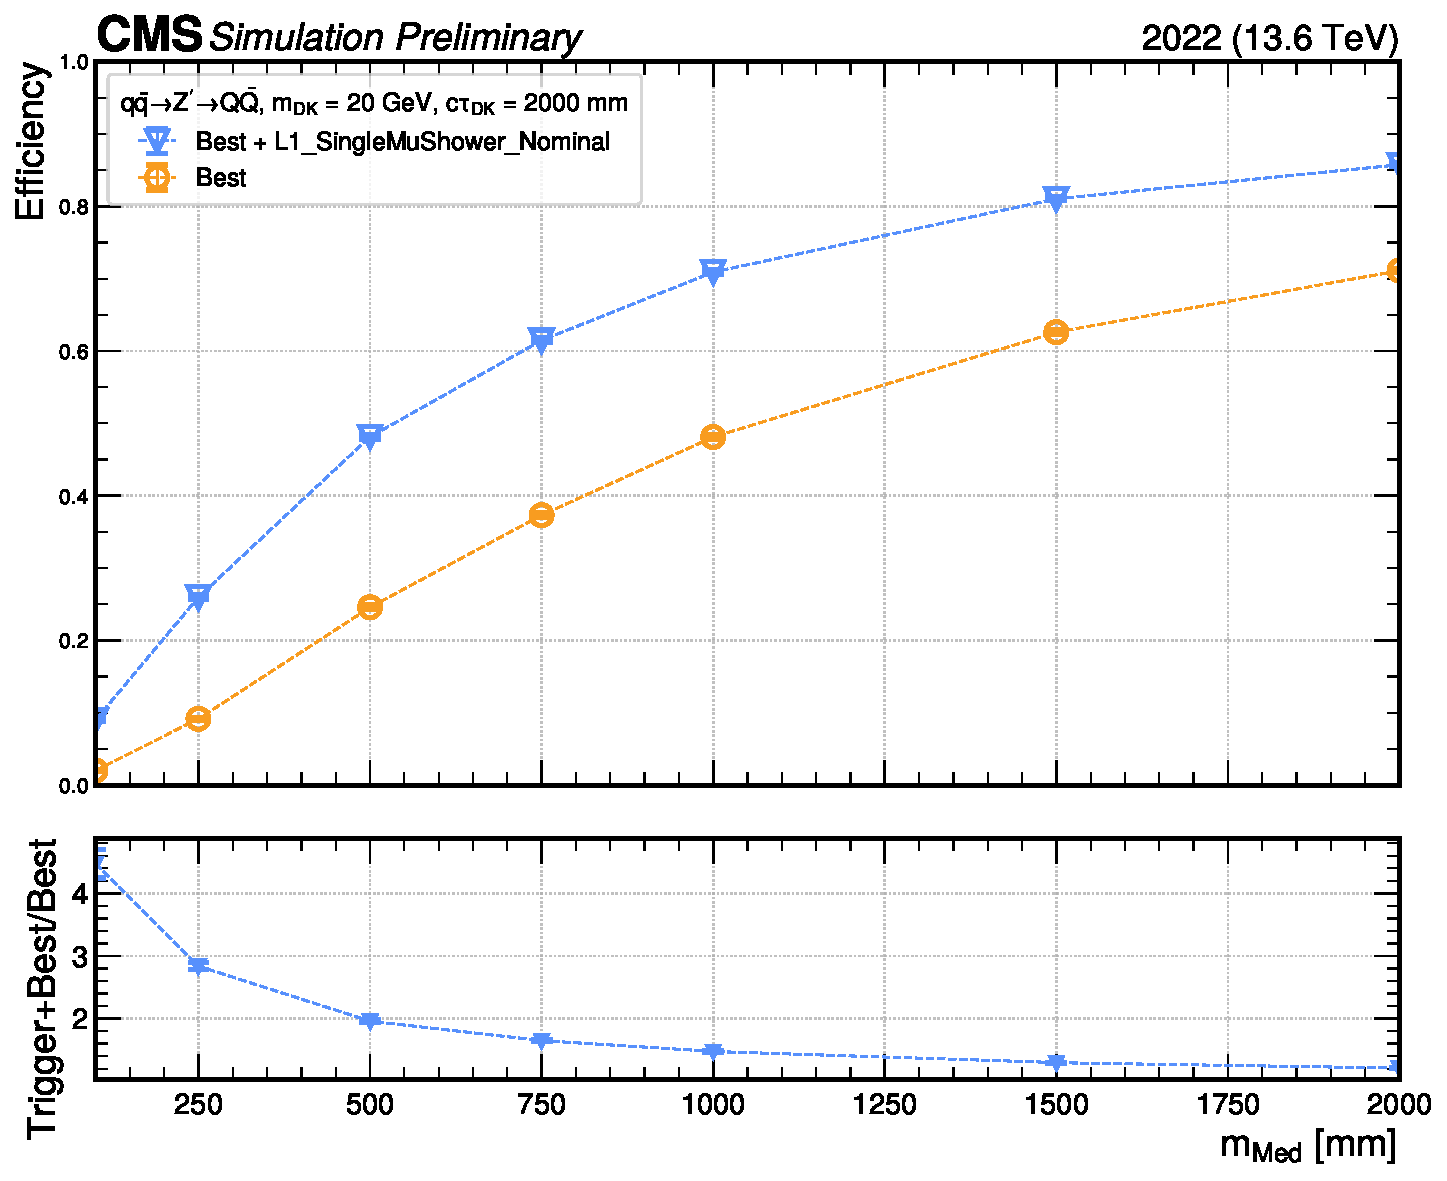
\includegraphics[width=\linewidth]{images/L1/llp_1D_schan/trigeffplots1D_L1_efftype-trigplusbest_s-channel_mDark-20_ctau-2000_L1_SingleMuShower_Nominal_study_cloppear.pdf}
    \caption{Trigger+best efficiency for $c\tau = 2000$ mm, Z' mediator model}
    \label{fig:mus_eff1D_ctau2000_schan}
  \end{subfigure}

  \vspace{1em}

  % Bifundamental mediator model (t-channel)
  \begin{subfigure}[t]{0.45\textwidth}
    \centering
    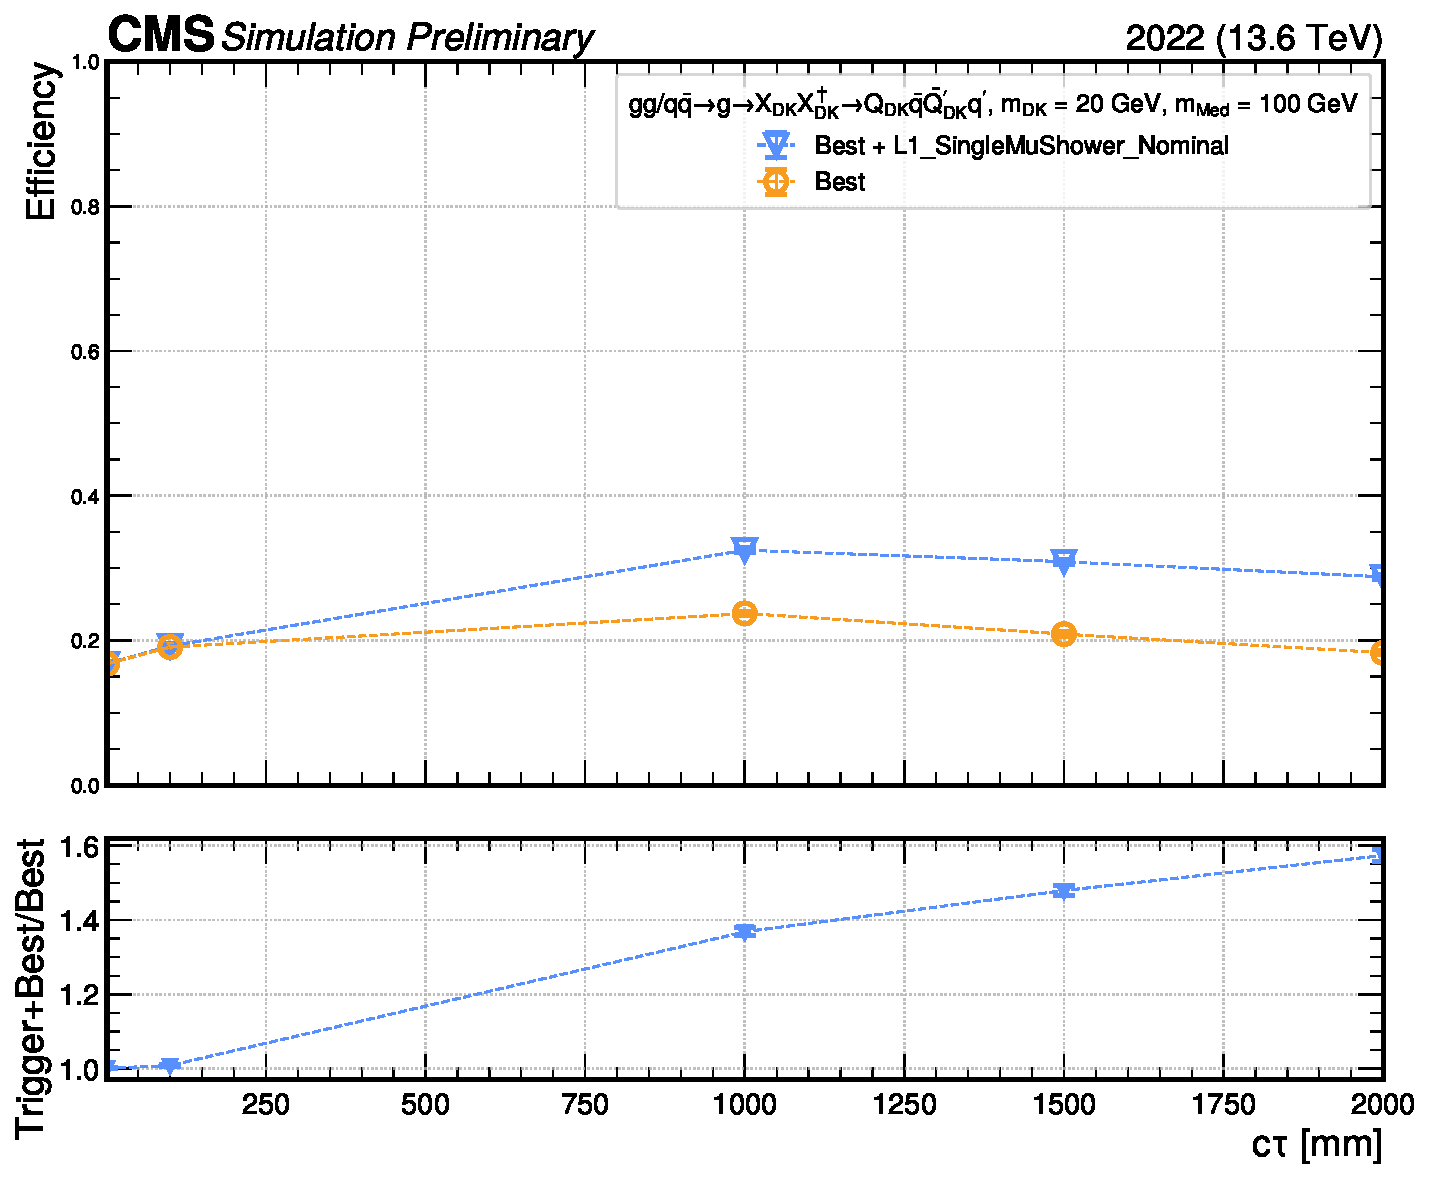
\includegraphics[width=\linewidth]{images/L1/llp_1D_tchan/trigeffplots1D_L1_efftype-trigplusbest_t-channel_mDark-20_mMed-100_L1_SingleMuShower_Nominal_study_cloppear.pdf}
    \caption{Trigger+best efficiency for $m_\mathrm{med} = 100$ GeV, Bifundamental mediator model}
    \label{fig:mus_eff1D_mmed100_tchan}
  \end{subfigure}
  \hfill
  % Z' mediator model (s-channel)
  \begin{subfigure}[t]{0.45\textwidth}
    \centering
    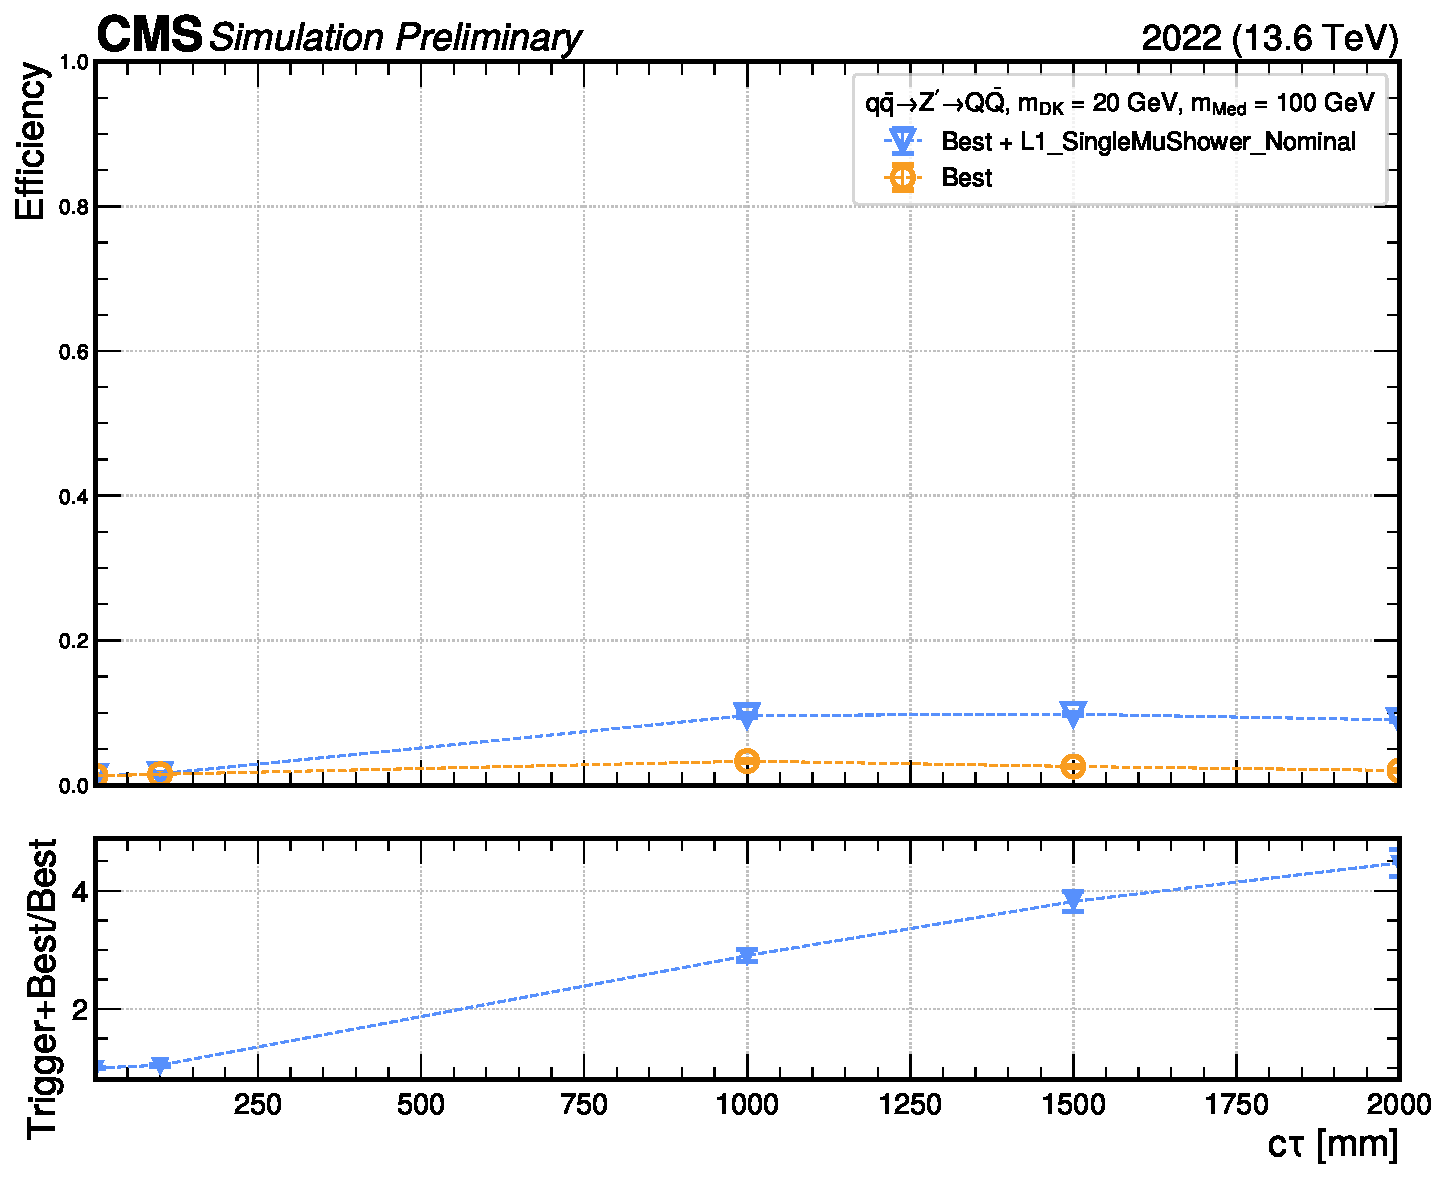
\includegraphics[width=\linewidth]{images/L1/llp_1D_schan/trigeffplots1D_L1_efftype-trigplusbest_s-channel_mDark-20_mMed-100_L1_SingleMuShower_Nominal_study_cloppear.pdf}
    \caption{Trigger+best efficiency for $m_\mathrm{med} = 100$ GeV, Z' mediator model}
    \label{fig:mus_eff1D_mmed100_schan}
  \end{subfigure}

  \caption{1D trigger+best object efficiency plots for \texttt{L1\_SingleMuShower\_Nominal} with $m_\mathrm{dark} = 20$ GeV. Each plot includes an efficiency curve and a ratio panel showing improvement. The values of $c\tau$ (top) and $m_\mathrm{med}$ (bottom) correspond to the points of peak improvement in the 2D efficiency maps for each mediator model (bifundamental and Z').}
  \label{fig:mus_eff1D}
\end{figure}

%---%---%---%---%---%---%---%---%---%---%---%---%---%---%---%---

\newpage

\begin{landscape}
    \begin{table}[]
        \centering
        \begin{tabular}{ll}
            \hline
            \textbf{Trigger} & \textbf{Description}\\
            \hline
            \texttt{L1\_AXO\_Nominal} (version 4) & AXOL1TL anomaly score > $25.9375$\\
            % \texttt{L1\_AXO\_Nominal} (version 3) & AXOL1TL anomaly score > $1161.25$\\
            \texttt{L1\_CICADA\_Nominal} (version 2.1.2) & CICADA anomaly score > $121.0$\\
            \texttt{L1\_DoubleLLPJet40} & Two jets flagged as LLP jets, with at least one of them having $>40 \text{ GeV}$ of energy.\\
            \texttt{L1\_HTT200\_SingleLLPJet60} & At least a single LLP jet with energy $> 60 \text{ GeV}$. $H_T >200 \text{ GeV}$.\\
            \texttt{L1\_SingleMuShower\_Nominal} & At least a single muon shower in the CSC of the muon system\\
            \hline
        \end{tabular}
        \caption{Level-1 Triggers studied}
        \label{tab:l1-trigs}
    \end{table}
    % \begin{table}[]
    %     \centering
    %     \begin{tabular}{ll}
    %         \hline
    %         \textbf{Trigger} & \textbf{Description}\\
    %         \hline
    %         \texttt{HLT\_HT170\_L1SingleLLPJet\_DisplacedDijet40\_DisplacedTrack} & \\
    %         \texttt{HLT\_HT200\_L1SingleLLPJet\_DisplacedDijet40\_DisplacedTrack} & \\
    %         \texttt{HLT\_HT200\_L1SingleLLPJet\_DisplacedDijet60\_DisplacedTrack} & \\
    %         \texttt{HLT\_HT270\_L1SingleLLPJet\_DisplacedDijet40\_DisplacedTrack} & \\
    %         \texttt{HLT\_HT320\_L1SingleLLPJet\_DisplacedDijet60\_Inclusive} & \\
    %         \texttt{HLT\_HT420\_L1SingleLLPJet\_DisplacedDijet60\_Inclusive} & \\
    %         \texttt{HLT\_HT200\_L1SingleLLPJet\_DelayedJet40\_SingleDelay1nsTrackless} & \\
    %         \texttt{HLT\_HT200\_L1SingleLLPJet\_DelayedJet40\_SingleDelay2nsInclusive} & \\
    %         \texttt{HLT\_HT200\_L1SingleLLPJet\_DelayedJet40\_DoubleDelay0p5nsTrackless} & \\
    %         \texttt{HLT\_HT200\_L1SingleLLPJet\_DelayedJet40\_DoubleDelay1nsInclusive} & \\
    %         \texttt{HLT\_HT200\_L1SingleLLPJet\_DisplacedDijet40\_Inclusive1PtrkShortSig5} &\\
    %         \hline
    %     \end{tabular}
    %     \caption{High-Level Triggers (HLT) studied}
    %     \label{tab:hlt-trigs}
    % \end{table}
\end{landscape}